\documentclass[12pt,openright,oneside]{book}

% Paquetes necesarios
\usepackage[spanish]{babel}        % Idioma español
\usepackage[utf8]{inputenc}        % Codificación UTF-8
\usepackage[T1]{fontenc}           % Codificación de salida
\usepackage{newtxtext,newtxmath}   % Fuente Times New Roman
\usepackage{setspace}              % Interlineado
\usepackage{geometry}              % Márgenes
\usepackage{titlesec}              % Formato de títulos
\usepackage{fancyhdr}              % Encabezados y pies de página
\usepackage{graphicx}              % Imágenes
\usepackage{tocloft}               % Formato del índice
\usepackage{hyperref}              % Hipervínculos
\hypersetup{colorlinks=true, linkcolor=black, urlcolor=blue} 
\usepackage{apacite}               % Citas y referencias APA
\usepackage{enumerate}             % Listas enumeradas
\usepackage{caption}               % Personalización de leyendas
\usepackage{subcaption}            % Subfiguras
\usepackage{longtable}             % Tablas largas
\usepackage{listings}              % Código fuente
\usepackage{pdfpages}              % Incluir PDF (para anexos)
\usepackage{color}                 % Colores
\usepackage{xcolor}                % Colores
\usepackage{float}
\usepackage{chngcntr}
\counterwithout{figure}{chapter}

% Configuración de márgenes
\geometry{
    left=3cm,
    right=2cm,
    top=4cm,
    bottom=3cm,
}

% Configuración de código fuente
% Configuración del paquete listings
\lstset{
    basicstyle=\ttfamily\small, % Estilo básico del código
    keywordstyle=\color{blue}\bfseries, % Estilo de las palabras clave
    commentstyle=\color{gray}\itshape, % Estilo de los comentarios
    stringstyle=\color{red}, % Estilo de las cadenas de texto
    numbers=left, % Números de línea a la izquierda
    numberstyle=\tiny\color{gray}, % Estilo de los números de línea
    stepnumber=1, % Numerar cada línea
    numbersep=5pt, % Separación entre el número y el código
    frame=single, % Marco alrededor del código
    framexleftmargin=15pt, % Margen izquierdo del marco
    xleftmargin=15pt, % Margen izquierdo del código
    captionpos=b, % Posición de la leyenda (caption) abajo
    breaklines=true, % Permitir saltos de línea
    breakatwhitespace=false, % Romper líneas en espacios en blanco
    showspaces=false, % No mostrar espacios en blanco
    showtabs=false, % No mostrar tabulaciones
    tabsize=2, % Tamaño de tabulación
    columns=fullflexible
}

% Interlineado 1.5 para todo el documento
\onehalfspacing

% Numeración de capítulos en números romanos y secciones en arábigos
\titleformat{\chapter}{\normalfont\huge\bfseries}{\Roman{chapter}.}{1em}{}
\titleformat{\section}{\normalfont\Large\bfseries}{\thesection.}{1em}{}

% Ajustes para el índice
\renewcommand{\contentsname}{ÍNDICE GENERAL}
\setlength{\cftbeforechapskip}{0pt}
\setlength{\cftbeforesecskip}{0pt}

% Encabezados y pies de página
\pagestyle{fancy}
\fancyhf{}
\renewcommand{\headrulewidth}{0pt}
\fancyfoot[C]{\thepage}

% En español, que diga "Figura" en lugar de "Figure"
\renewcommand{\figurename}{Figura}

% Configuración de tablas y figuras
\captionsetup[table]{font=normalsize,skip=0pt,singlelinecheck=false}

% Ajustar espacio antes/después de la leyenda
\setlength{\abovecaptionskip}{8pt}   % espacio entre imagen y leyenda si la leyenda va debajo
\setlength{\belowcaptionskip}{0pt}  % espacio después de la leyenda

\captionsetup[figure]{%
  position=above,                       % Coloca la leyenda (número y título) encima de la imagen
  labelfont=bf,                         % "Figura X." en negrita
  labelsep=newline,                     % Salto de línea tras "Figura X."
  textfont=it,                          % Título en cursiva
  font={normalsize,stretch=1.5},         % Interlineado de 1.5 para cumplir APA
  skip=10pt,                            % Espacio entre la leyenda y la imagen (ajusta este valor según lo requieras)
  justification=justified,
  singlelinecheck=false
}

% Configuración de citas y referencias APA
\bibliographystyle{apacite}
\renewcommand{\APACrefYearMonthDay}[3]{\APACrefYear{#1}}

\begin{document}
% Configuración de numeración de páginas para las secciones preliminares
\pagenumbering{Roman}
\setcounter{page}{1}

% Portada
\begin{titlepage}
    \begin{center}
        \vspace*{2cm}
        {\Large\textbf{SISTEMA DE DETECCIÓN TEMPRANA DE BOTRYTIS CINEREA EN EL ARÁNDANO BILOXI MEDIANTE TERMOGRAFÍA}}\\[4cm]
        {\large\textbf{AUTOR(ES)}}\\
        Juan Esteban Fuentes Rojas\\
        Gabriel Esteban Martinez Roldan\\[6cm]
        \textbf{UNIVERSIDAD DE CUNDINAMARCA}\\
        Facultad de Ingeniería\\
        Programa de Ingeniería de Sistemas y Computación\\
        Facatativá, Noviembre 2025
    \end{center}
\end{titlepage}

% Contraportada
\newpage
\thispagestyle{empty}
\begin{center}
    \vspace*{2cm}
    {\Large\textbf{SISTEMA DE DETECCIÓN TEMPRANA DE BOTRYTIS CINEREA EN EL ARÁNDANO BILOXI MEDIANTE TERMOGRAFÍA}}\\[3cm]
    {\large\textbf{AUTOR(ES)}}\\
    Directora: Ing. Gina Maribel Valenzuela Sabogal\\
    Juan Esteban Fuentes Rojas\\
    Gabriel Esteban Martinez Roldan\\[3cm]
    \textbf{GRUPO DE INVESTIGACIÓN DE SISTEMAS Y TECNOLOGÍA DE FACATATIVÁ (GISTFA)}\\[3cm]
    \textbf{UNIVERSIDAD DE CUNDINAMARCA}\\
    Facultad de Ingeniería\\
    Programa de Ingeniería de Sistemas\\
    Facatativá, Noviembre 2025
\end{center}

% Dedicatoria (opcional)
\chapter*{Dedicatoria}
\addcontentsline{toc}{chapter}{Dedicatoria}
Texto de la dedicatoria...

% Agradecimientos (opcional)
\chapter*{Agradecimientos}
\addcontentsline{toc}{chapter}{Agradecimientos}
Texto de los agradecimientos...

% Compromiso de Autor (Anexo final, incluir si es necesario)

% Resumen y Palabras Clave
\chapter*{Resumen}
\addcontentsline{toc}{chapter}{Resumen}

% Interlineado sencillo para el resumen
\begin{spacing}{1}
    Texto del resumen en español (200 a 250 palabras, sin sangría).
\end{spacing}

\vspace{1cm}

\textbf{Palabras clave:} palabra1, palabra2, palabra3, palabra4, palabra5.

\newpage  % Nueva página para el abstract y keywords

% Abstract and Keywords
\chapter*{Abstract}
\addcontentsline{toc}{chapter}{Abstract}

% Interlineado sencillo para el abstract
\begin{spacing}{1}
    Texto del resumen en inglés (200 a 250 palabras, sin sangría).
\end{spacing}

\vspace{1cm}

\textbf{Keywords:} keyword1, keyword2, keyword3, keyword4, keyword5.

\newpage  % Nueva página para el índice general

% Índice General
\tableofcontents
\newpage

% Lista de Tablas
\listoftables
\addcontentsline{toc}{chapter}{Lista de Tablas}
\newpage

% Lista de Figuras
\listoffigures
\addcontentsline{toc}{chapter}{Lista de Figuras}
\newpage

% Lista de Anexos (si aplica)
\chapter*{Lista de Anexos}
\addcontentsline{toc}{chapter}{Lista de Anexos}
\begin{enumerate}
    \item Anexo A: Título del Anexo A
    \item Anexo B: Título del Anexo B
    % Agregar más anexos si es necesario
\end{enumerate}

% Introducción
\chapter*{Introducción}
\addcontentsline{toc}{chapter}{Introducción}
Texto de la introducción (2 a 4 páginas).

% Cuerpo del Documento
\mainmatter
\setcounter{page}{1}

% Capítulo I: Informe de Investigación
\doublespacing
\chapter{INFORME DE INVESTIGACIÓN}

\section{Estado del Arte}
Texto del estado del arte...

\section{Línea de Investigación}
Texto de la línea de investigación...

\section{Planteamiento del Problema y Pregunta de Investigación}
La producción de arándanos está en aumento debido a su alta demanda, siendo la variedad Biloxi la que más se cultiva en el altiplano cundiboyacense según datos de Quintana (2020). Sin embargo, la planta requiere condiciones específicas de temperatura para dar fruto. La falta de estas condiciones la hace susceptible a enfermedades, representando un desafío significativo para los productores. Sin un manejo oportuno, las enfermedades pueden causar la muerte de las plantas, afectando el cultivo y provocando pérdidas económicas. Esto subraya la importancia de una gestión adecuada, reflejada en las exportaciones de frutos del género Vaccinium en Colombia, que alcanzaron los 2,2 millones de dólares, según la Asociación Nacional de Comercio Exterior (ANALDEX, 2022).

\bigskip
Respecto a las enfermedades en plantas (fitopatologías), Quintana afirma que la Botrytis Cinerea es una de las más comunes en el arándano. La Botryotinia Fuckeliana (fase asexuada: Botrytis Cinerea), comúnmente conocida como Botrytis o moho gris, es una enfermedad fúngica que afecta una amplia variedad de plantas, incluyendo la planta de arándano Biloxi (Quintana, 2020). Esta enfermedad es particularmente destructiva en condiciones de alta humedad y temperaturas moderadas, promoviendo la formación de esporas. Los síntomas típicos de la Botrytis incluyen manchas marrones en hojas, flores y frutos, que eventualmente se cubren de un moho gris característico. En las hojas, causa lesiones de color café que comienzan generalmente por el centro de la lámina y se extienden hacia los bordes, produciendo una necrosis extensiva. En condiciones de alta humedad, sobre las lesiones de las hojas se desarrollan las estructuras reproductivas del patógeno (conidióforos y conidios), que dan un aspecto plomizo (grisáceo o plateado) en los tejidos (Morales, et al. 2017).

\bigskip
Una técnica no invasiva ampliamente utilizada en agricultura para monitorear la salud de las plantas es la termografía infrarroja (IRT), permitiendo además gestionar el riego, detectar enfermedades y estimar la producción (Dong et al., 2024; Aux et al., 2022). Esta herramienta es fundamental para avanzar hacia una agricultura más automatizada, precisa y sostenible, permitiendo supervisar el estrés térmico en cultivos y analizar el impacto de patógenos en la transpiración de las plantas. Aunque la investigación demuestra que la IRT está superando sus limitaciones y se está convirtiendo en un método robusto, confiable y económico para determinar el estado hídrico de las plantas y detectar el estrés (Pineda et al., 2020), su alto costo actual restringe su uso principalmente a grupos de investigación y empresas especializadas (García Tejero et al., 2015).

\bigskip
Teniendo en cuenta las afectaciones de la Botrytis a los cultivos de arándano, es crucial explorar métodos no invasivos como la termografía. Si la termografía permite hacer una detección temprana de esta enfermedad se podría mejorar la gestión de la salud del cultivo y reducir las pérdidas. Lo cual plantea la pregunta, ¿Cómo desarrollar un sistema para aproximar la detección temprana de Botrytis Cinerea en plantas de arándanos Biloxi mediante hardware de bajo costo?


\section{Objetivo General y Objetivos Específicos}
\subsection{Objetivo General}
Desarrollar un sistema de detección aproximada de Botrytis Cinerea en plantas de arándano Biloxi utilizando termografía infrarroja (IRT) mediante hardware de bajo costo.

\subsection{Objetivos Específicos}
\begin{enumerate}
    \item Identificar y documentar los requisitos funcionales y no funcionales del sistema.
    \item Modelar la arquitectura del sistema mediante la creación de diagramas UML.
    \item Integrar el hardware del módulo termográfico para la recolección de datos.
    \item Desarrollar el software que recolecte los datos del módulo termográfico para su posterior procesamiento.
    \item Analizar los datos obtenidos en plantas infectadas por Botrytis Cinerea y plantas saludables para determinar la precisión del sistema desarrollado.
\end{enumerate}

\section{ Alcance e Impacto del Proyecto }
El presente proyecto busca ser un apoyo a la producción de arándanos a través de la implementación de tecnologías de precisión, como la termografía, para monitorear y gestionar la salud de los cultivos. Esto podría permitir a los agricultores minimizar las perdidas en los cultivos y poder “satisfacer los desafíos de seguridad alimentaria local, regional y global del siglo XXI” (Vargas Q. \& Best S., 2021).

\bigskip
La agricultura tecnificada y precisa es más sostenible porque permite utilizar recursos de manera óptima, como la utilización de fitosanitarios solo donde sea necesario. Según Manuel Pérez-Ruiz, director del máster en Agricultura Digital e Innovación Agroalimentaria de la Universidad de Sevilla, esta forma de agricultura también ayuda a que los agricultores sean más competitivos y no abandonen su territorio (Communications, 2024).
Este proyecto está alineado con los Objetivos de Desarrollo Sostenible (ODS), específicamente con el ODS 9, que busca promover la inversión en infraestructura y la innovación para impulsar el crecimiento económico y el desarrollo sostenible. También contribuye a reducir la huella ecológica mediante la gestión eficiente de los recursos naturales compartidos y la implementación de prácticas agrícolas sostenibles, lo que se relaciona con el ODS 12.

\bigskip
La implementación de este proyecto puede tener un impacto significativo en la seguridad alimentaria y la economía local. Al reducir las pérdidas económicas en la producción de cultivos y al promover la eficiencia energética, podemos crear cadenas de producción y suministro más eficientes. Además, el acceso a tecnologías de precisión puede ayudar a reducir la brecha digital entre países desarrollados y en desarrollo, lo que se relaciona con el ODS 9.


\section{Metodología}
\subsection{Metodología de Investigación}
Para llevar a cabo esta investigación se utilizará la metodología de investigación mixta, la cual combina la perspectiva cuantitativa y cualitativa, lo que permite dar profundidad al análisis y comprender mejor los procesos. Esto implica recopilar, analizar e interpretar datos tanto cualitativos como cuantitativos para obtener una visión más completa de la problemática a estudiar. Esta metodología busca compensar las limitaciones de cada enfoque al mismo tiempo que fortalece la validez de la interpretación de los resultados (Hamui-Sutton, 2013).

\bigskip
La metodología mixta en este proyecto se empleará con el fin de combinar la recopilación y análisis de datos cuantitativos, como las lecturas de temperatura obtenidas a través del módulo de cámara térmica, con la exploración cualitativa de los resultados, como la descripción de las características en las plantas de arándano biloxi. Además de los datos termográficos, también se tomarán en cuenta otras variables importantes para el crecimiento de la planta y el hongo, buscando así tener una visión más completa de los factores que influyen en su desarrollo.Esto permitirá obtener una vista más amplia de la problemática a estudiar, comprendiendo así la relación entre las lecturas termográficas y la presencia de Botrytis Cinerea, además de aquellos factores que puedan influir en la precisión del sistema.


\subsection{Metodología de Desarrollo}
Para el desarrollo del sistema, se adoptarán elementos del marco de trabajo ágil Scrum, un enfoque de desarrollo iterativo y colaborativo diseñado para fomentar la adaptabilidad y la entrega continua de valor. Este método, reconocido por su flexibilidad y eficiencia, se basa en ciclos cortos de trabajo llamados Sprints, que permiten planificar, ejecutar y revisar tareas de manera organizada y dinámica (SCRUMstudy™, 2022).

\bigskip
Durante el proyecto, se trabajará en Sprints semanales, en los cuales se evaluarán los avances del Product Backlog previamente definido. Esta estructura facilita la retroalimentación constante, priorización de tareas y ajustes según las necesidades del proyecto, asegurando un desarrollo estructurado y orientado a cumplir los objetivos establecidos. La implementación de Scrum permitirá un desarrollo funcional que cumpla con las expectativas de precisión y eficacia requeridas.

\section{Marcos de Referencia}
\subsection{Marco Teórico}
Texto del marco teórico...

\subsection{Marco Legal}
Texto del marco legal...   % Capítulo I: Informe de Investigación
% Capítulo II: Documentación del Software
\chapter{DOCUMENTACIÓN DEL SOFTWARE}

% =================================================
% =================================================

\section{Plan de Proyecto}
Texto del plan de proyecto...

% =================================================
% =================================================

\section{Arquitectura del Software}

Describe la estructura global del sistema, mostrando cómo se organizan e interconectan los componentes del frontend y backend.

\subsection{Desarrollo del Frontend}
Documenta la implementación de la interfaz de usuario, detallando las tecnologías utilizadas y el diseño de la experiencia de usuario.

\subsection{Desarrollo del Backend}
Explica la lógica del servidor, la estructura de las APIs, la gestión de bases de datos y la implementación de la lógica de negocio que sustenta la aplicación.

\subsection{Integración Frontend-Backend}
Detalla los mecanismos y protocolos (por ejemplo, REST o WebSockets) que permiten la comunicación y sincronización de datos entre la interfaz y el servidor.

% =================================================
% =================================================

\section{Determinación de Requerimientos}
Texto sobre la determinación de requerimientos según formato IEEE...

% =================================================
% =================================================

\section{Especificación del Diseño}

\subsection{Modelo de Entidad-Relación (MER)}
\begin{figure}[H]
    \centering
    \caption{Diagrama Entidad-Relación del Sistema.}
    \label{fig:der}
    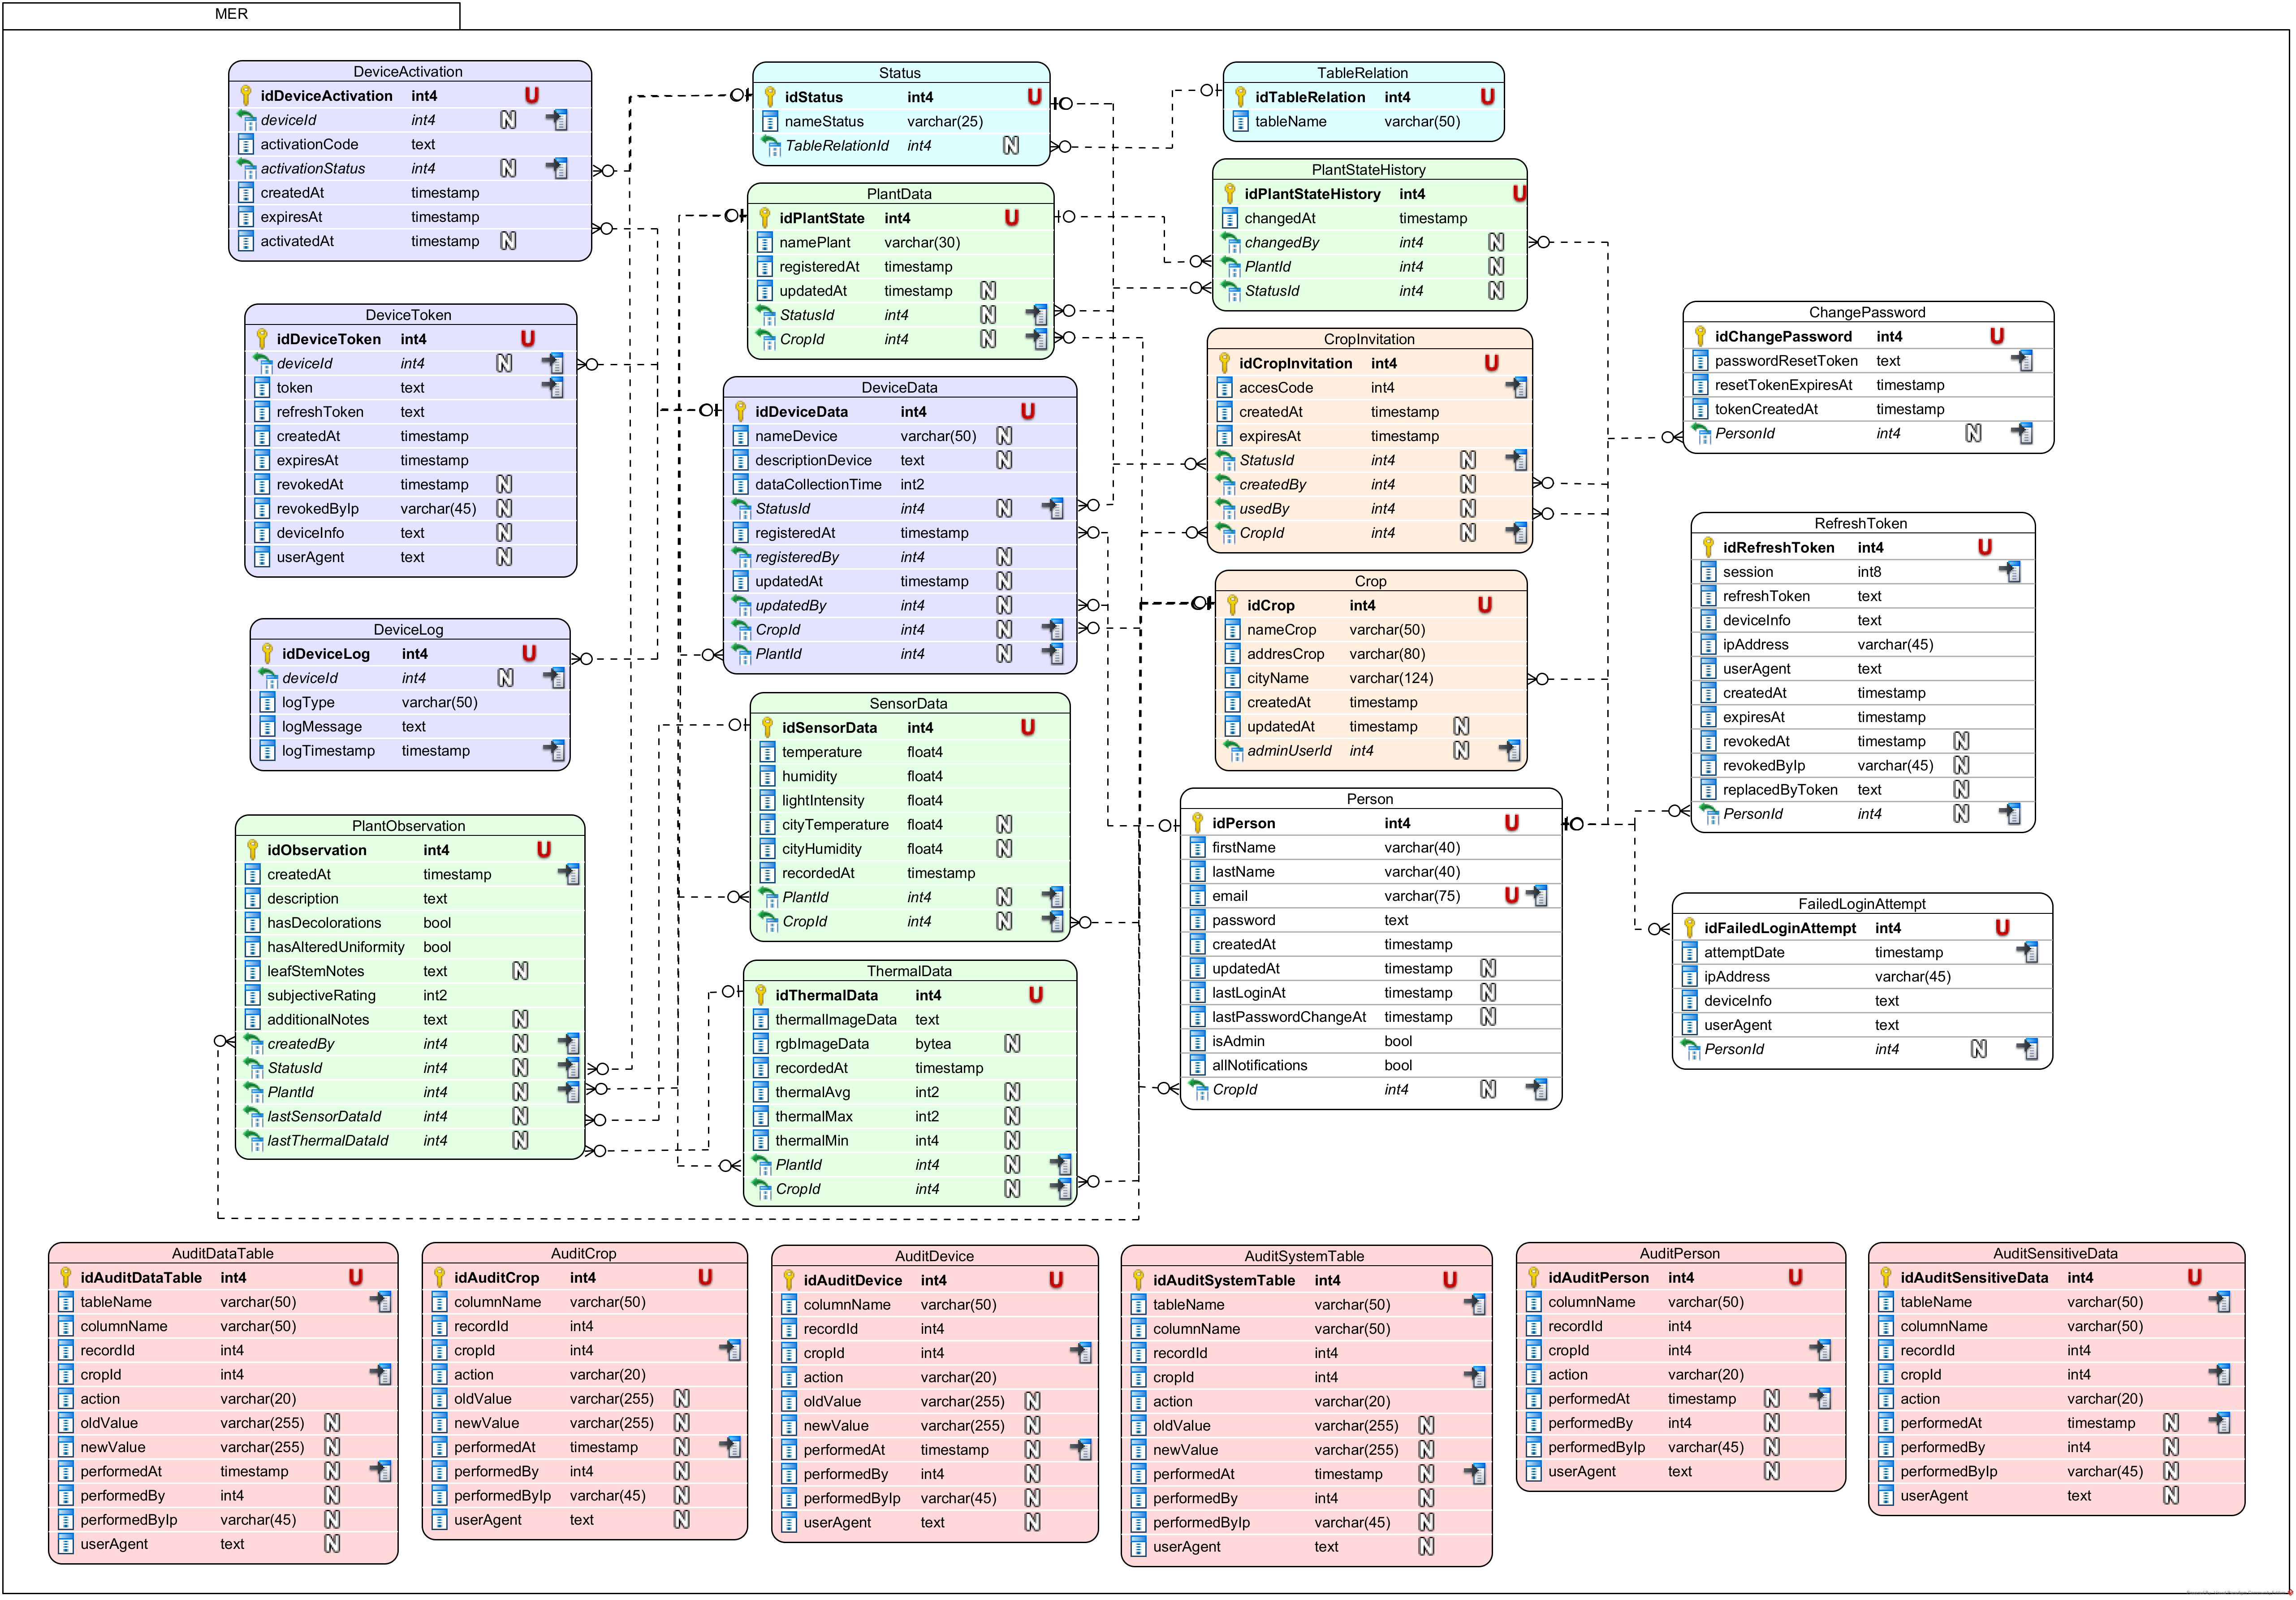
\includegraphics[width=1\textwidth]{UML/Otros/Diagrama Entidad Relacion.png}
\end{figure}

% =================================================
% =================================================

\subsection{Diagramas de Casos de Uso}

\begin{figure}[H]
    \centering
    \caption{Diagrama de Casos de Uso para la Gestión de Usuarios (RF1, RF2).}
    \label{fig:casos-uso-usuarios} % Opcional: Etiqueta para referencias
    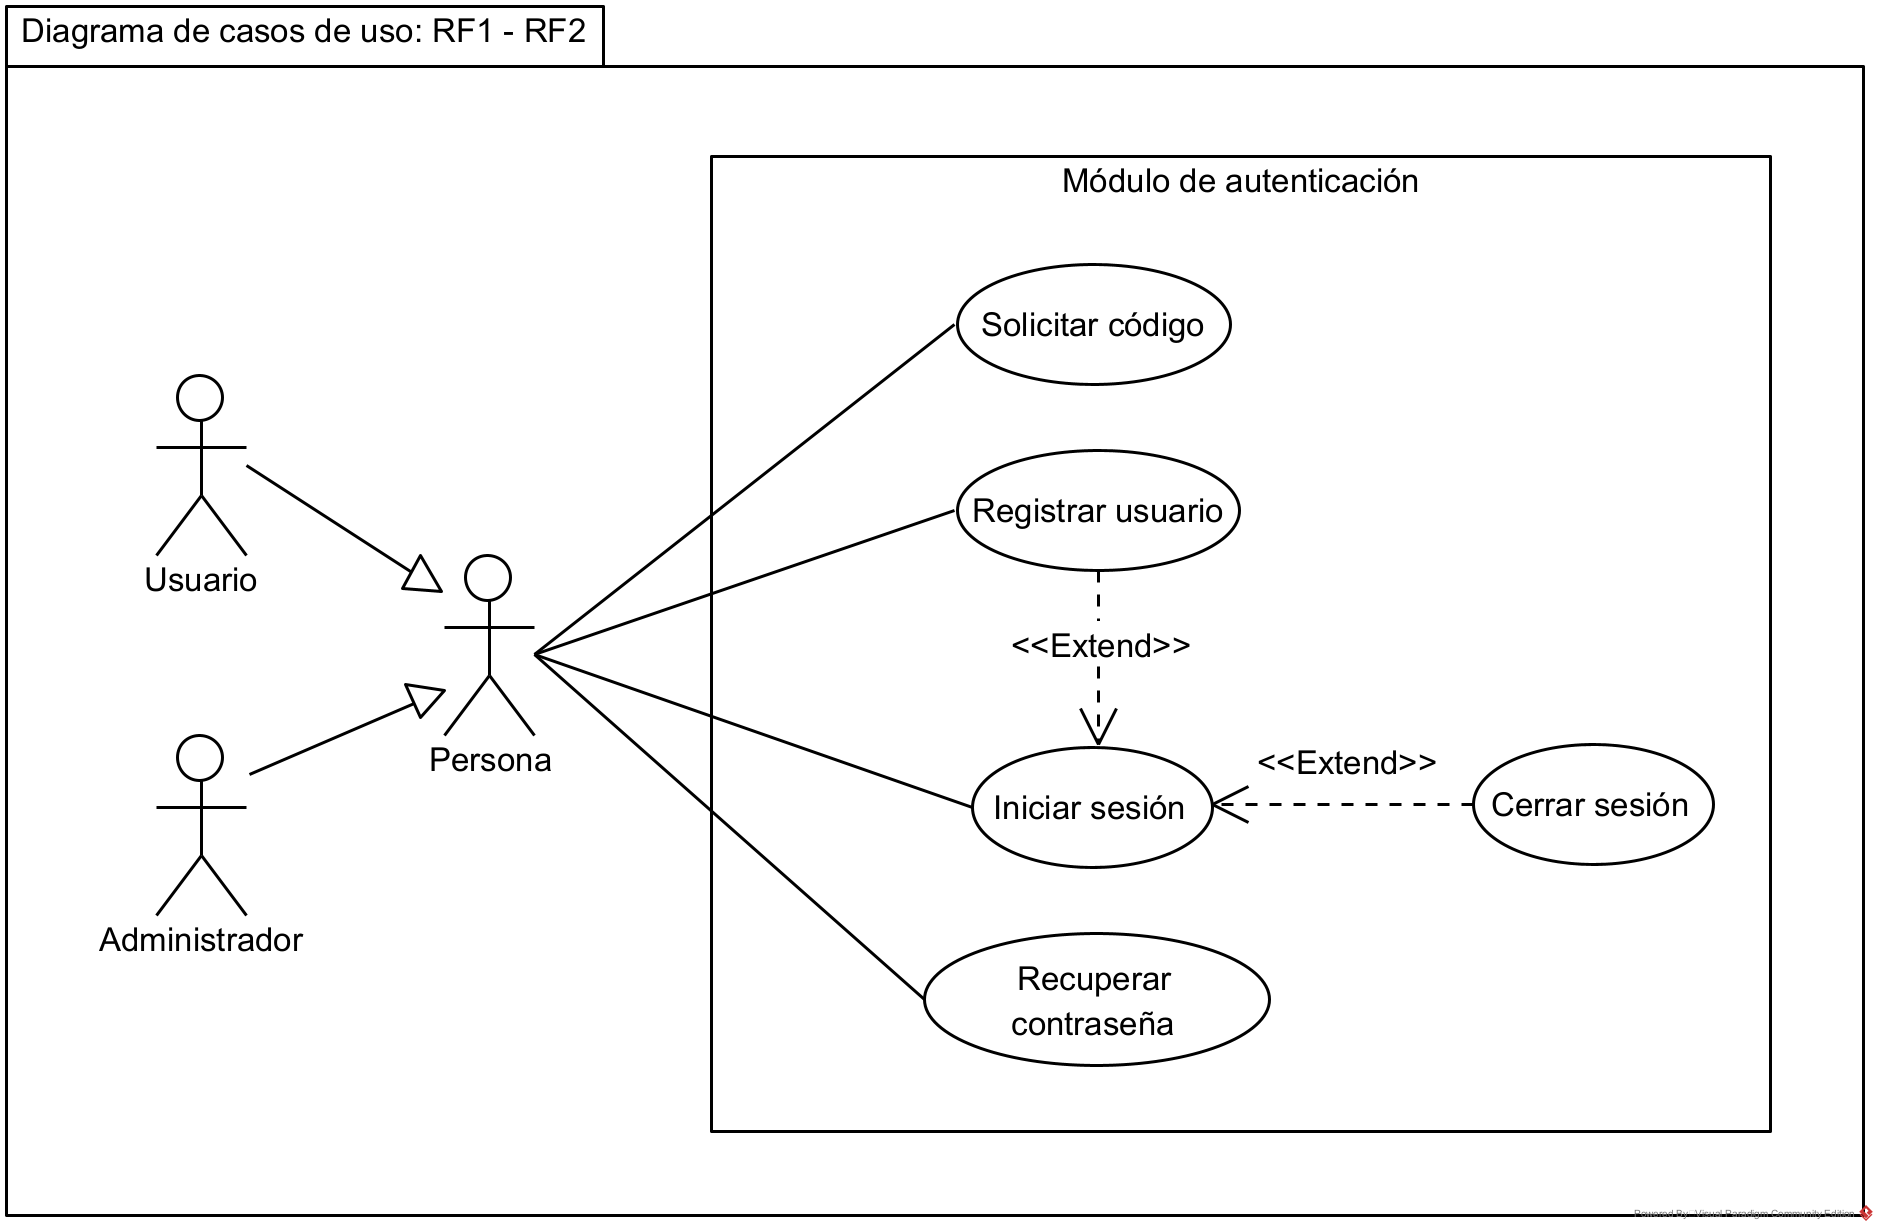
\includegraphics[width=0.8\textwidth]{UML/CasosUso/Diagrama de Casos de Uso RF1 RF2.png}
\end{figure}


\begin{figure}[H]
    \centering
    \caption{Diagrama de Casos de Uso para la Gestión de Cámaras (RF3).}
    \label{fig:casos-uso-camaras}
     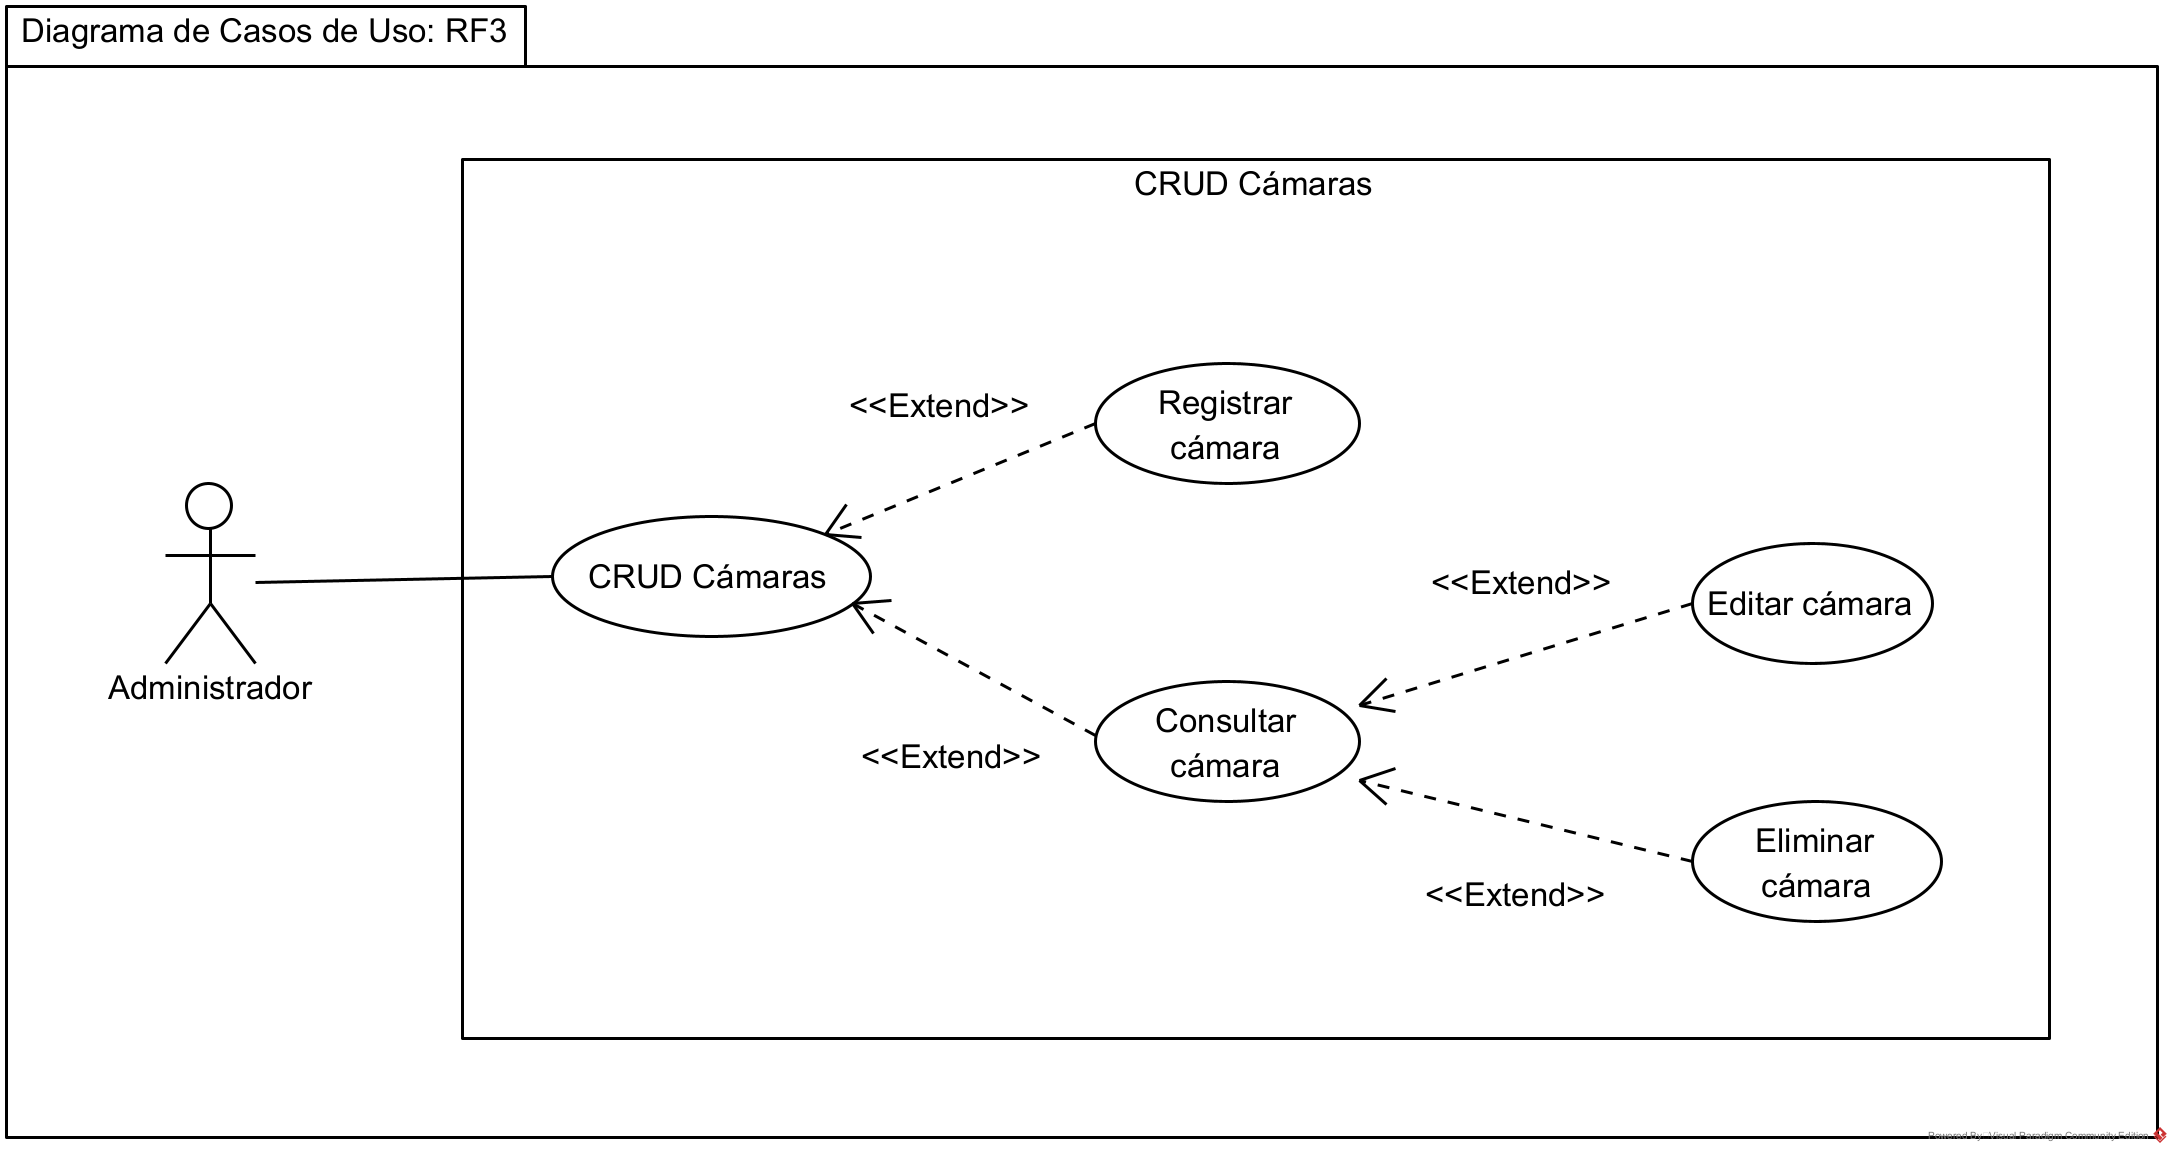
\includegraphics[width=0.8\textwidth]{UML/CasosUso/Diagrama de Casos de Uso RF3.png}
\end{figure}


\begin{figure}[H]
    \centering
    \caption{Diagrama de Casos de Uso para la Gestión de Perfiles (RF4).}
    \label{fig:casos-uso-perfiles}
    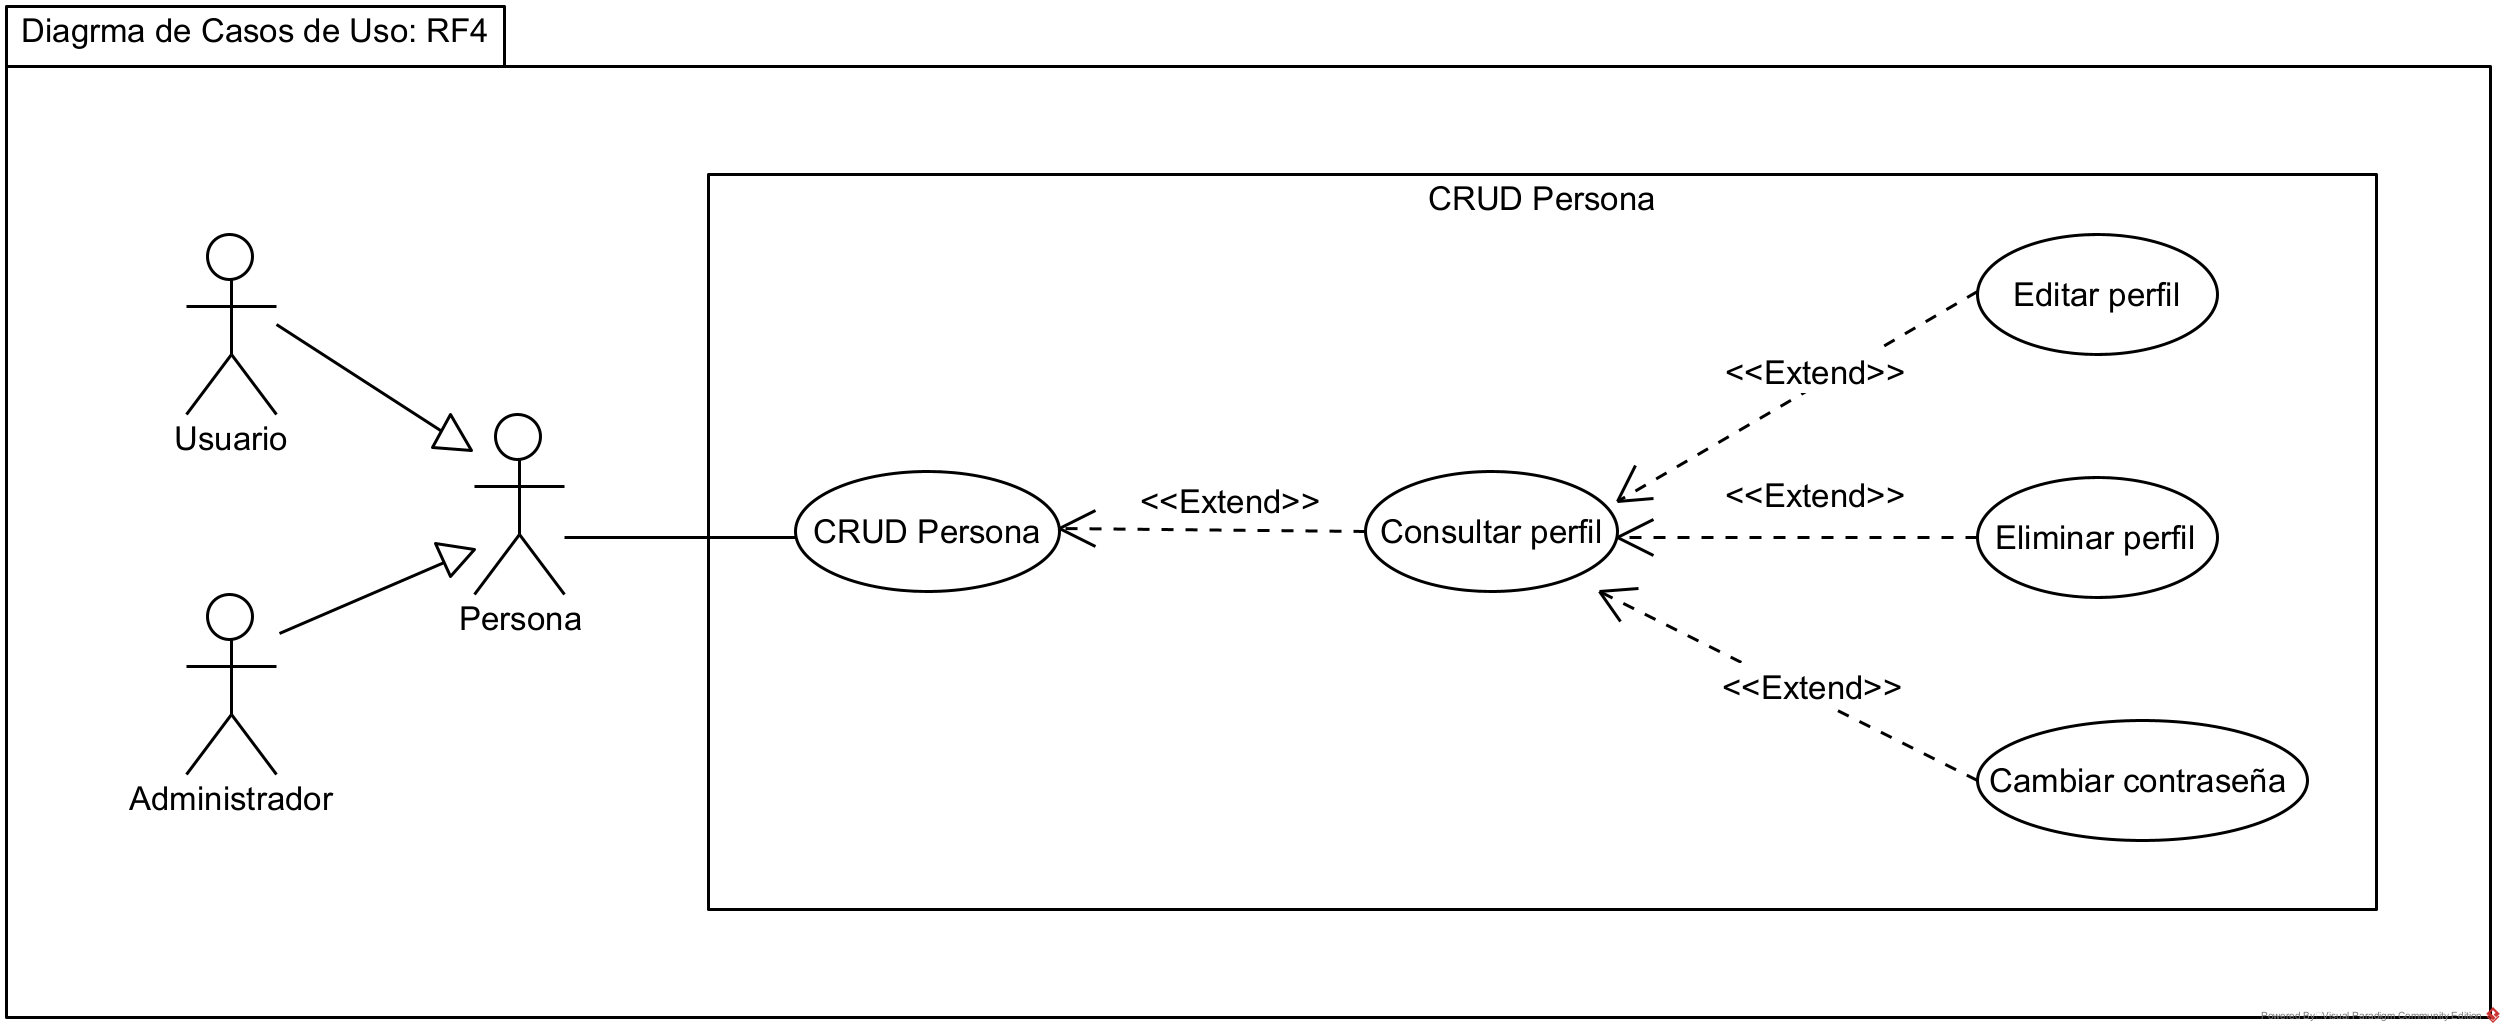
\includegraphics[width=0.8\textwidth]{UML/CasosUso/Diagrama de Casos de Uso RF4.png}
\end{figure}


\begin{figure}[H]
    \centering
    \caption{Diagrama de Casos de Uso para el Módulo de Mediciones (RF5).}
    \label{fig:casos-uso-mediciones}
    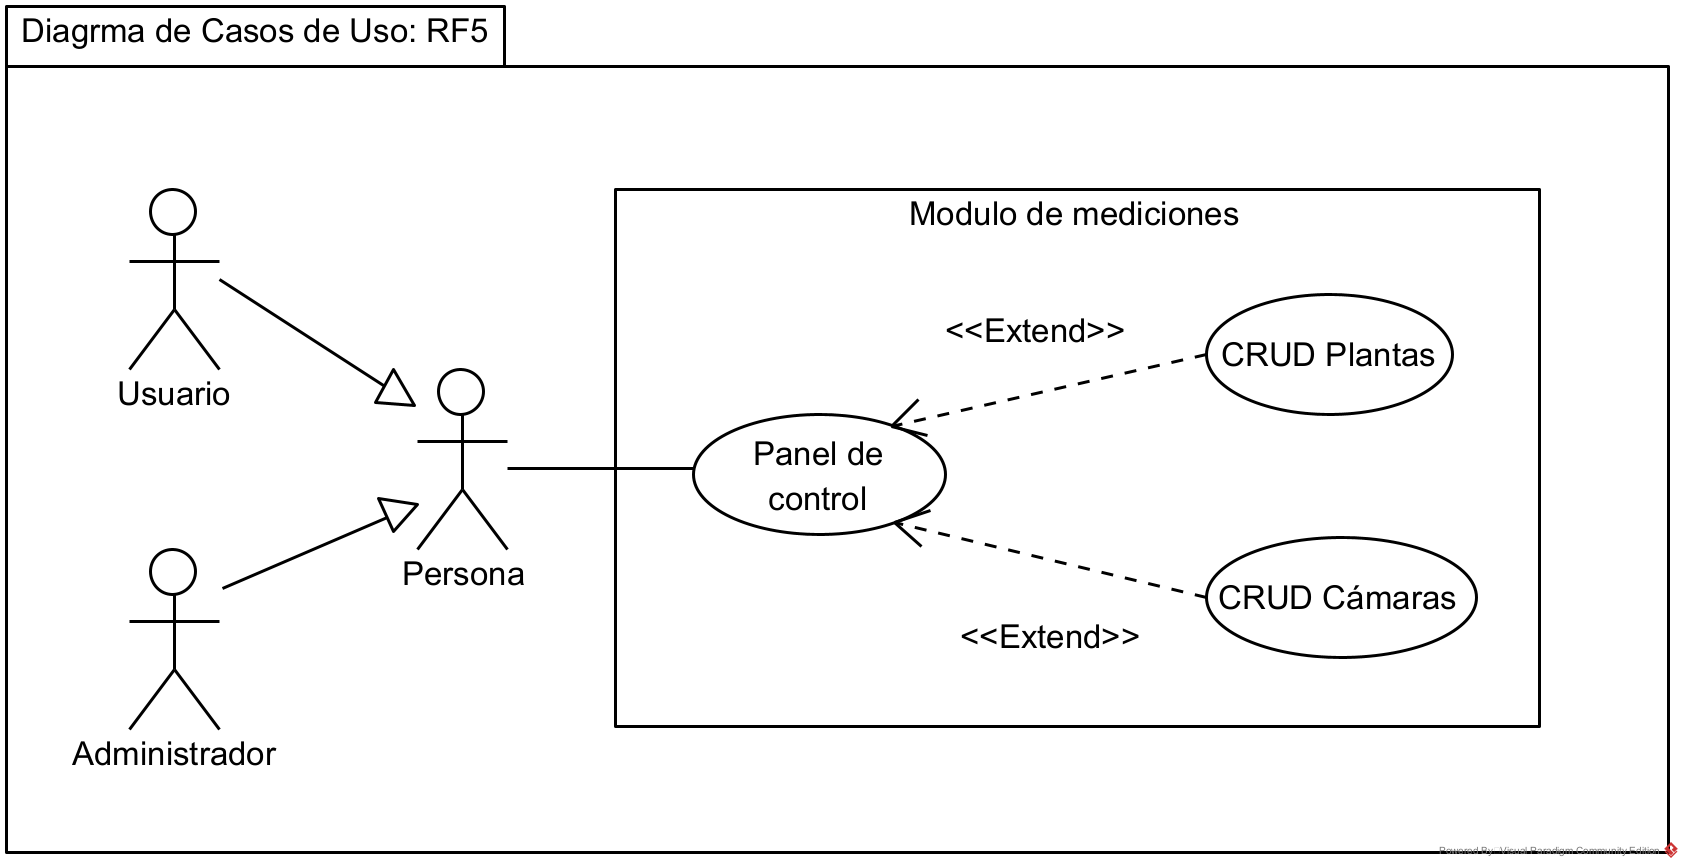
\includegraphics[width=0.8\textwidth]{UML/CasosUso/Diagrama de Casos de Uso RF5.png}
\end{figure}


\begin{figure}[H]
    \centering
    \caption{Diagrama de Casos de Uso para la Gestión de Plantas (RF6).}
    \label{fig:casos-uso-plantas}
    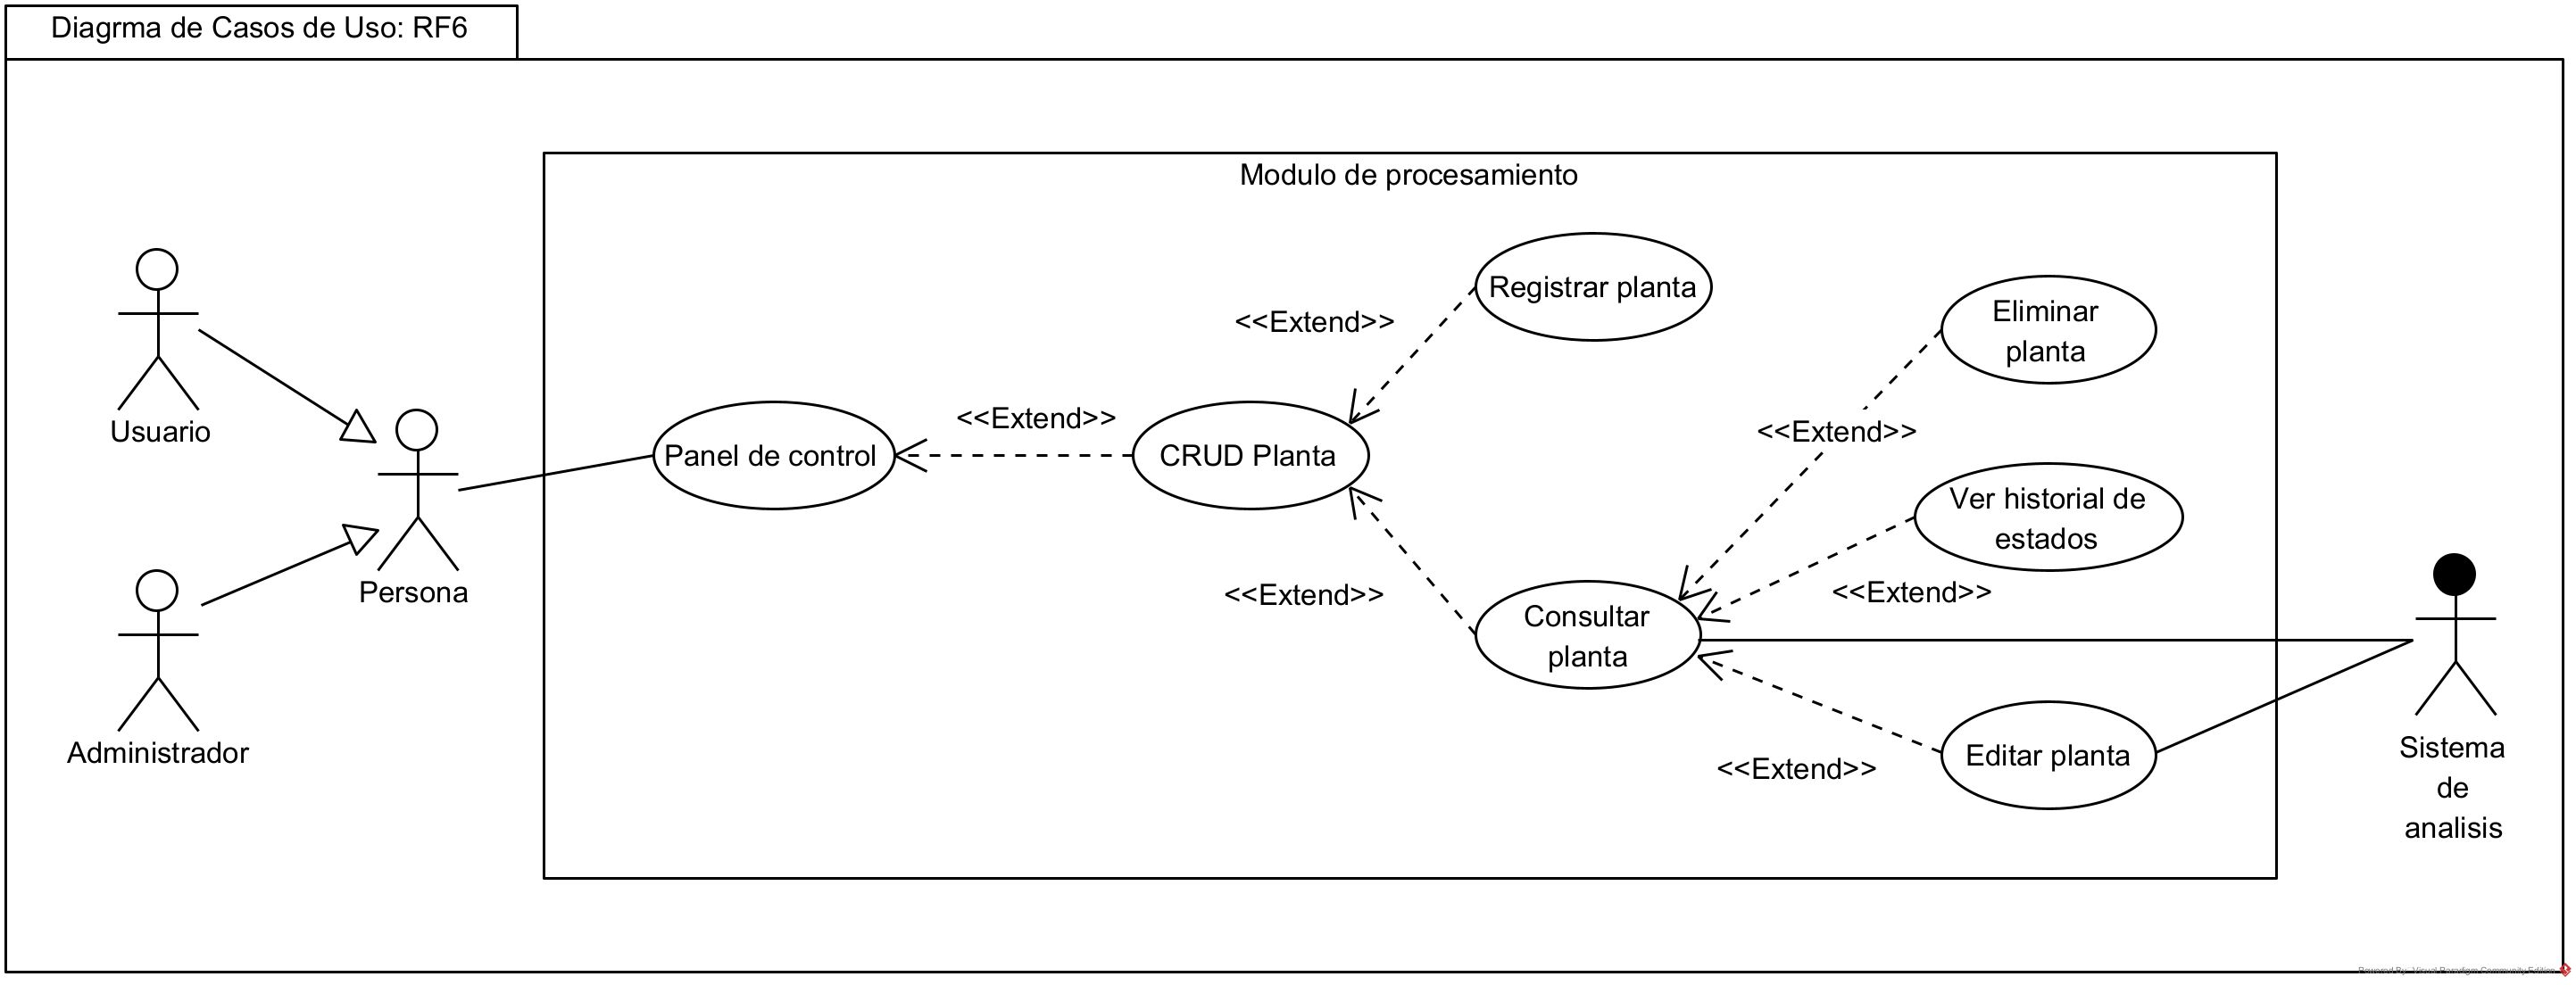
\includegraphics[width=0.8\textwidth]{UML/CasosUso/Diagrama de Casos de Uso RF6.png}
\end{figure}


\begin{figure}[H]
    \centering
    \caption{Diagrama de Casos de Uso para la Generación de Reportes (RF7).}
    \label{fig:casos-uso-reportes}
     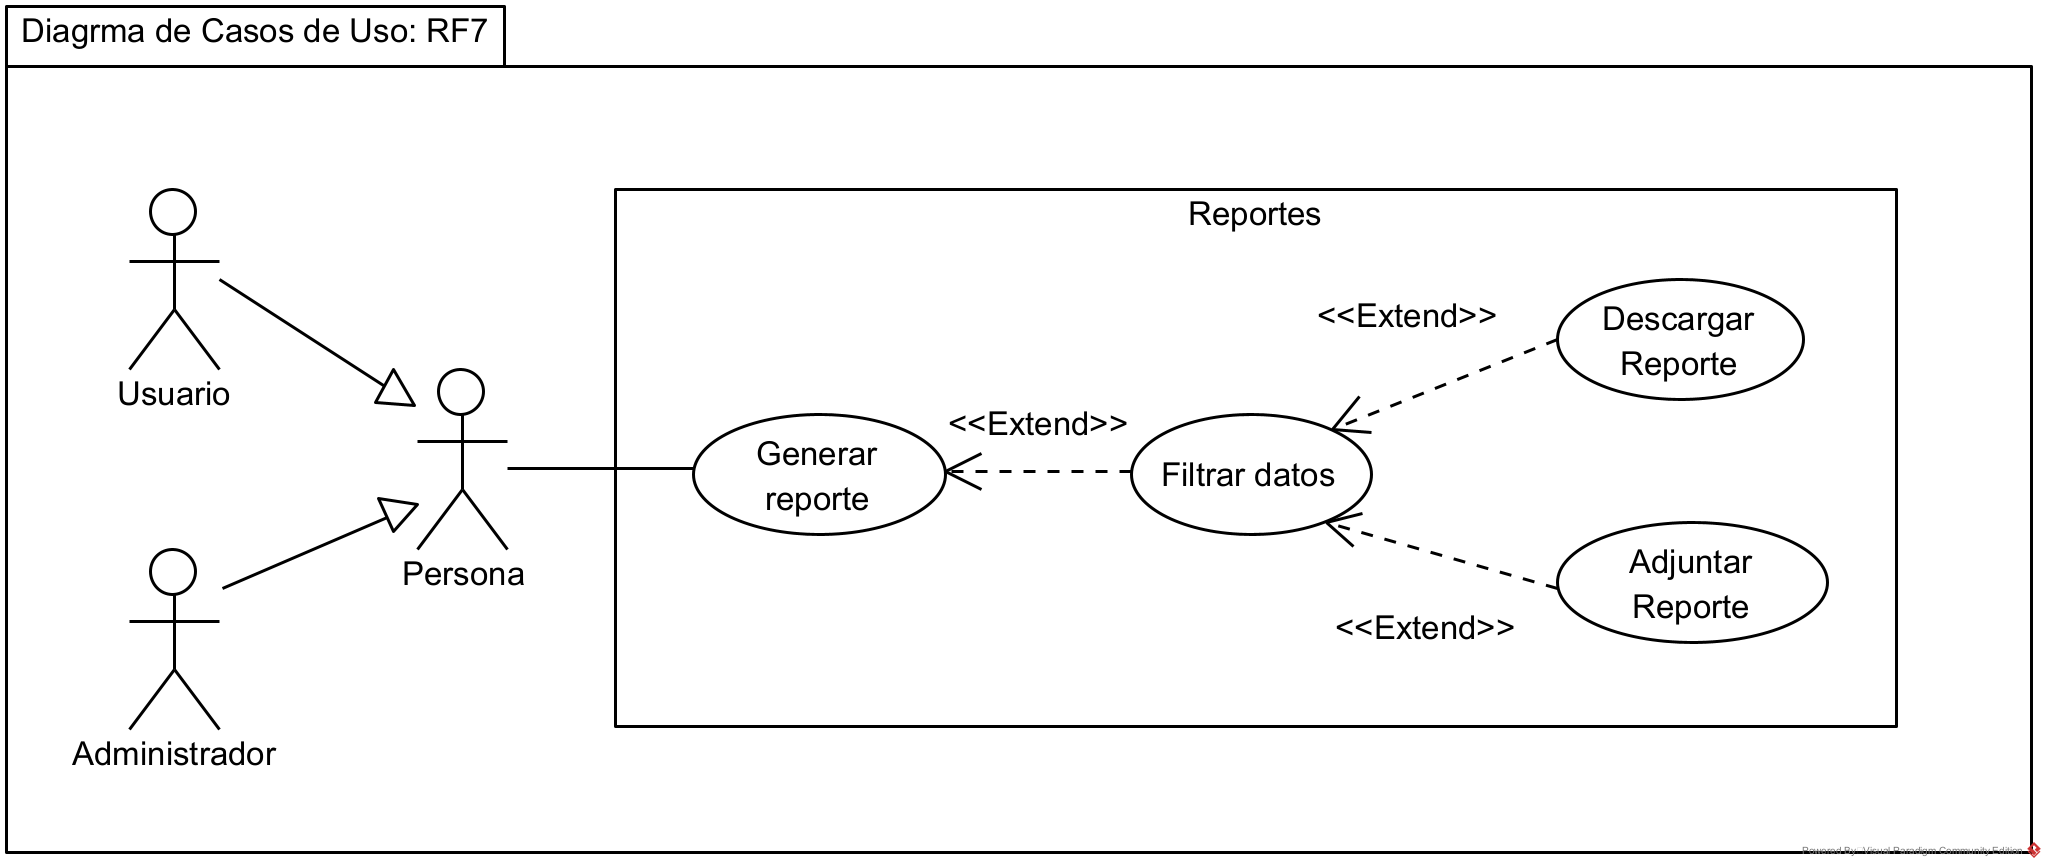
\includegraphics[width=0.8\textwidth]{UML/CasosUso/Diagrama de Casos de Uso RF7.png}
\end{figure}


\begin{figure}[H]
    \centering
    \caption{Diagrama de Casos de Uso para las Notificaciones (RF8).}
    \label{fig:casos-uso-notificaciones}
    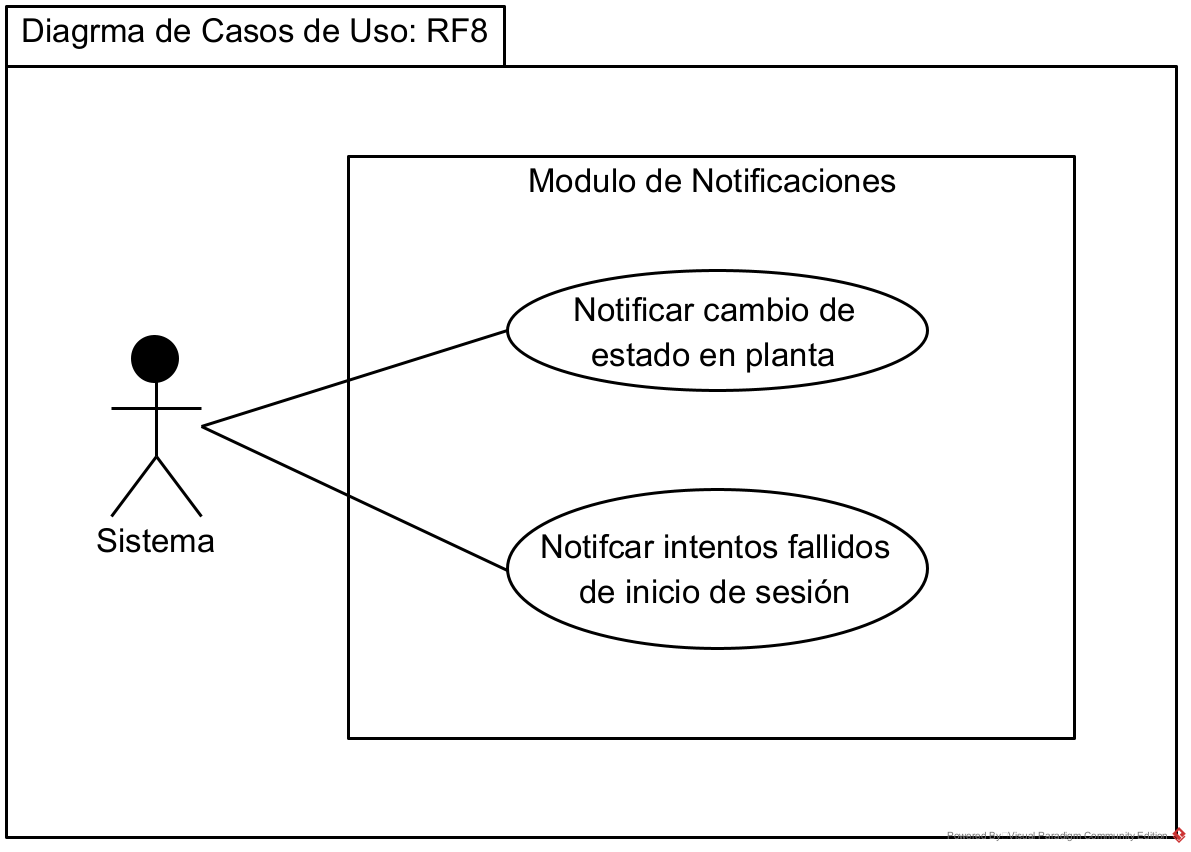
\includegraphics[width=0.8\textwidth]{UML/CasosUso/Diagrama de Casos de Uso RF8.png}
\end{figure}


\begin{figure}[H]
    \centering
    \caption{Diagrama de Casos de Uso para el Módulo de Observaciones (RF9).}
    \label{fig:casos-uso-observaciones}
    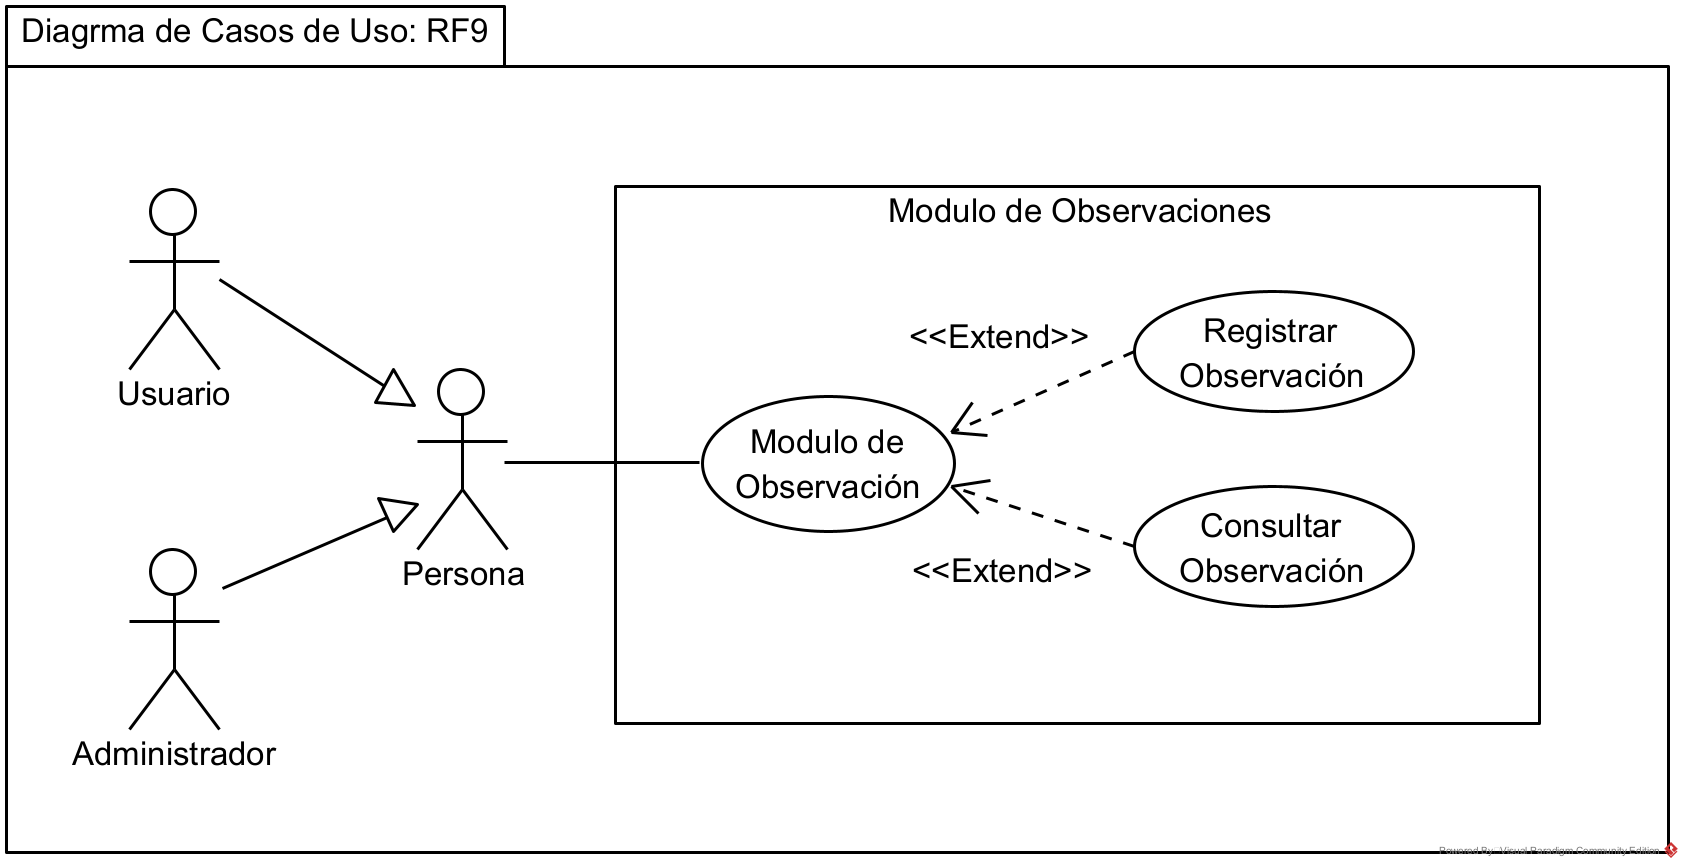
\includegraphics[width=0.8\textwidth]{UML/CasosUso/Diagrama de Casos de Uso RF9.png}
\end{figure}

% =================================================
% =================================================

\subsection{Diagramas de Secuencia}


\begin{figure}[H]
    \centering
    \caption{Diagrama de secuencia base: Envío de formulario.}
    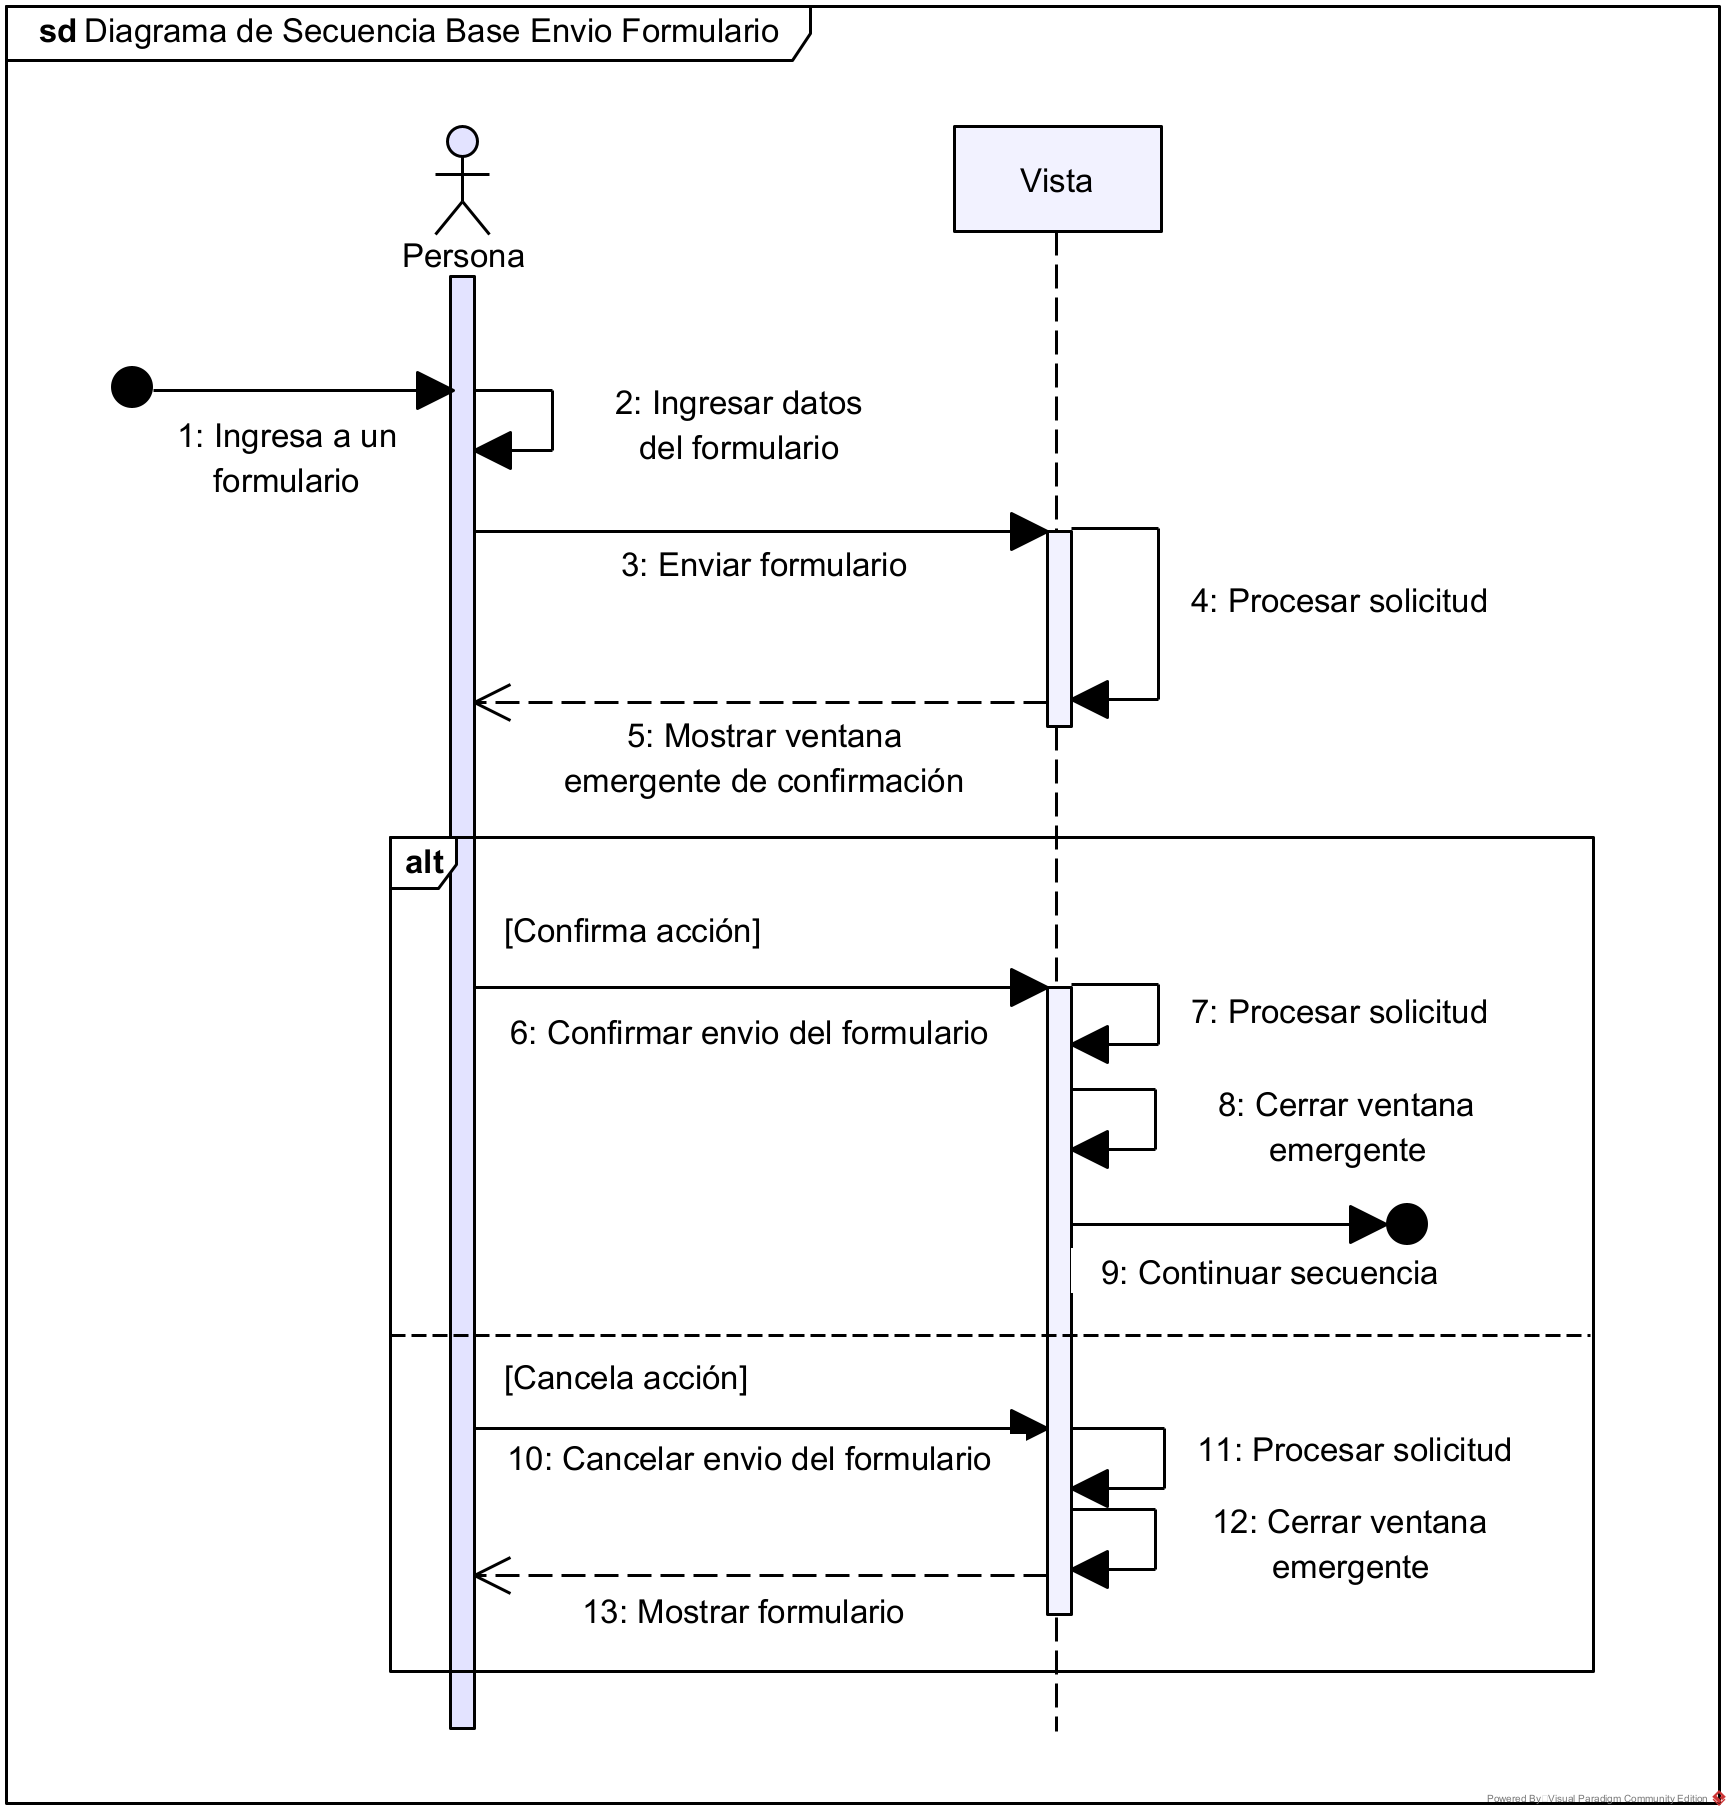
\includegraphics[width=0.8\textwidth]{UML/Secuencia/Diagrama de Secuencia Base Envio Formulario.png}
\end{figure}


\begin{figure}[H]
    \centering
    \caption{Diagrama de Secuencia para el Registro (RF1.0).}
 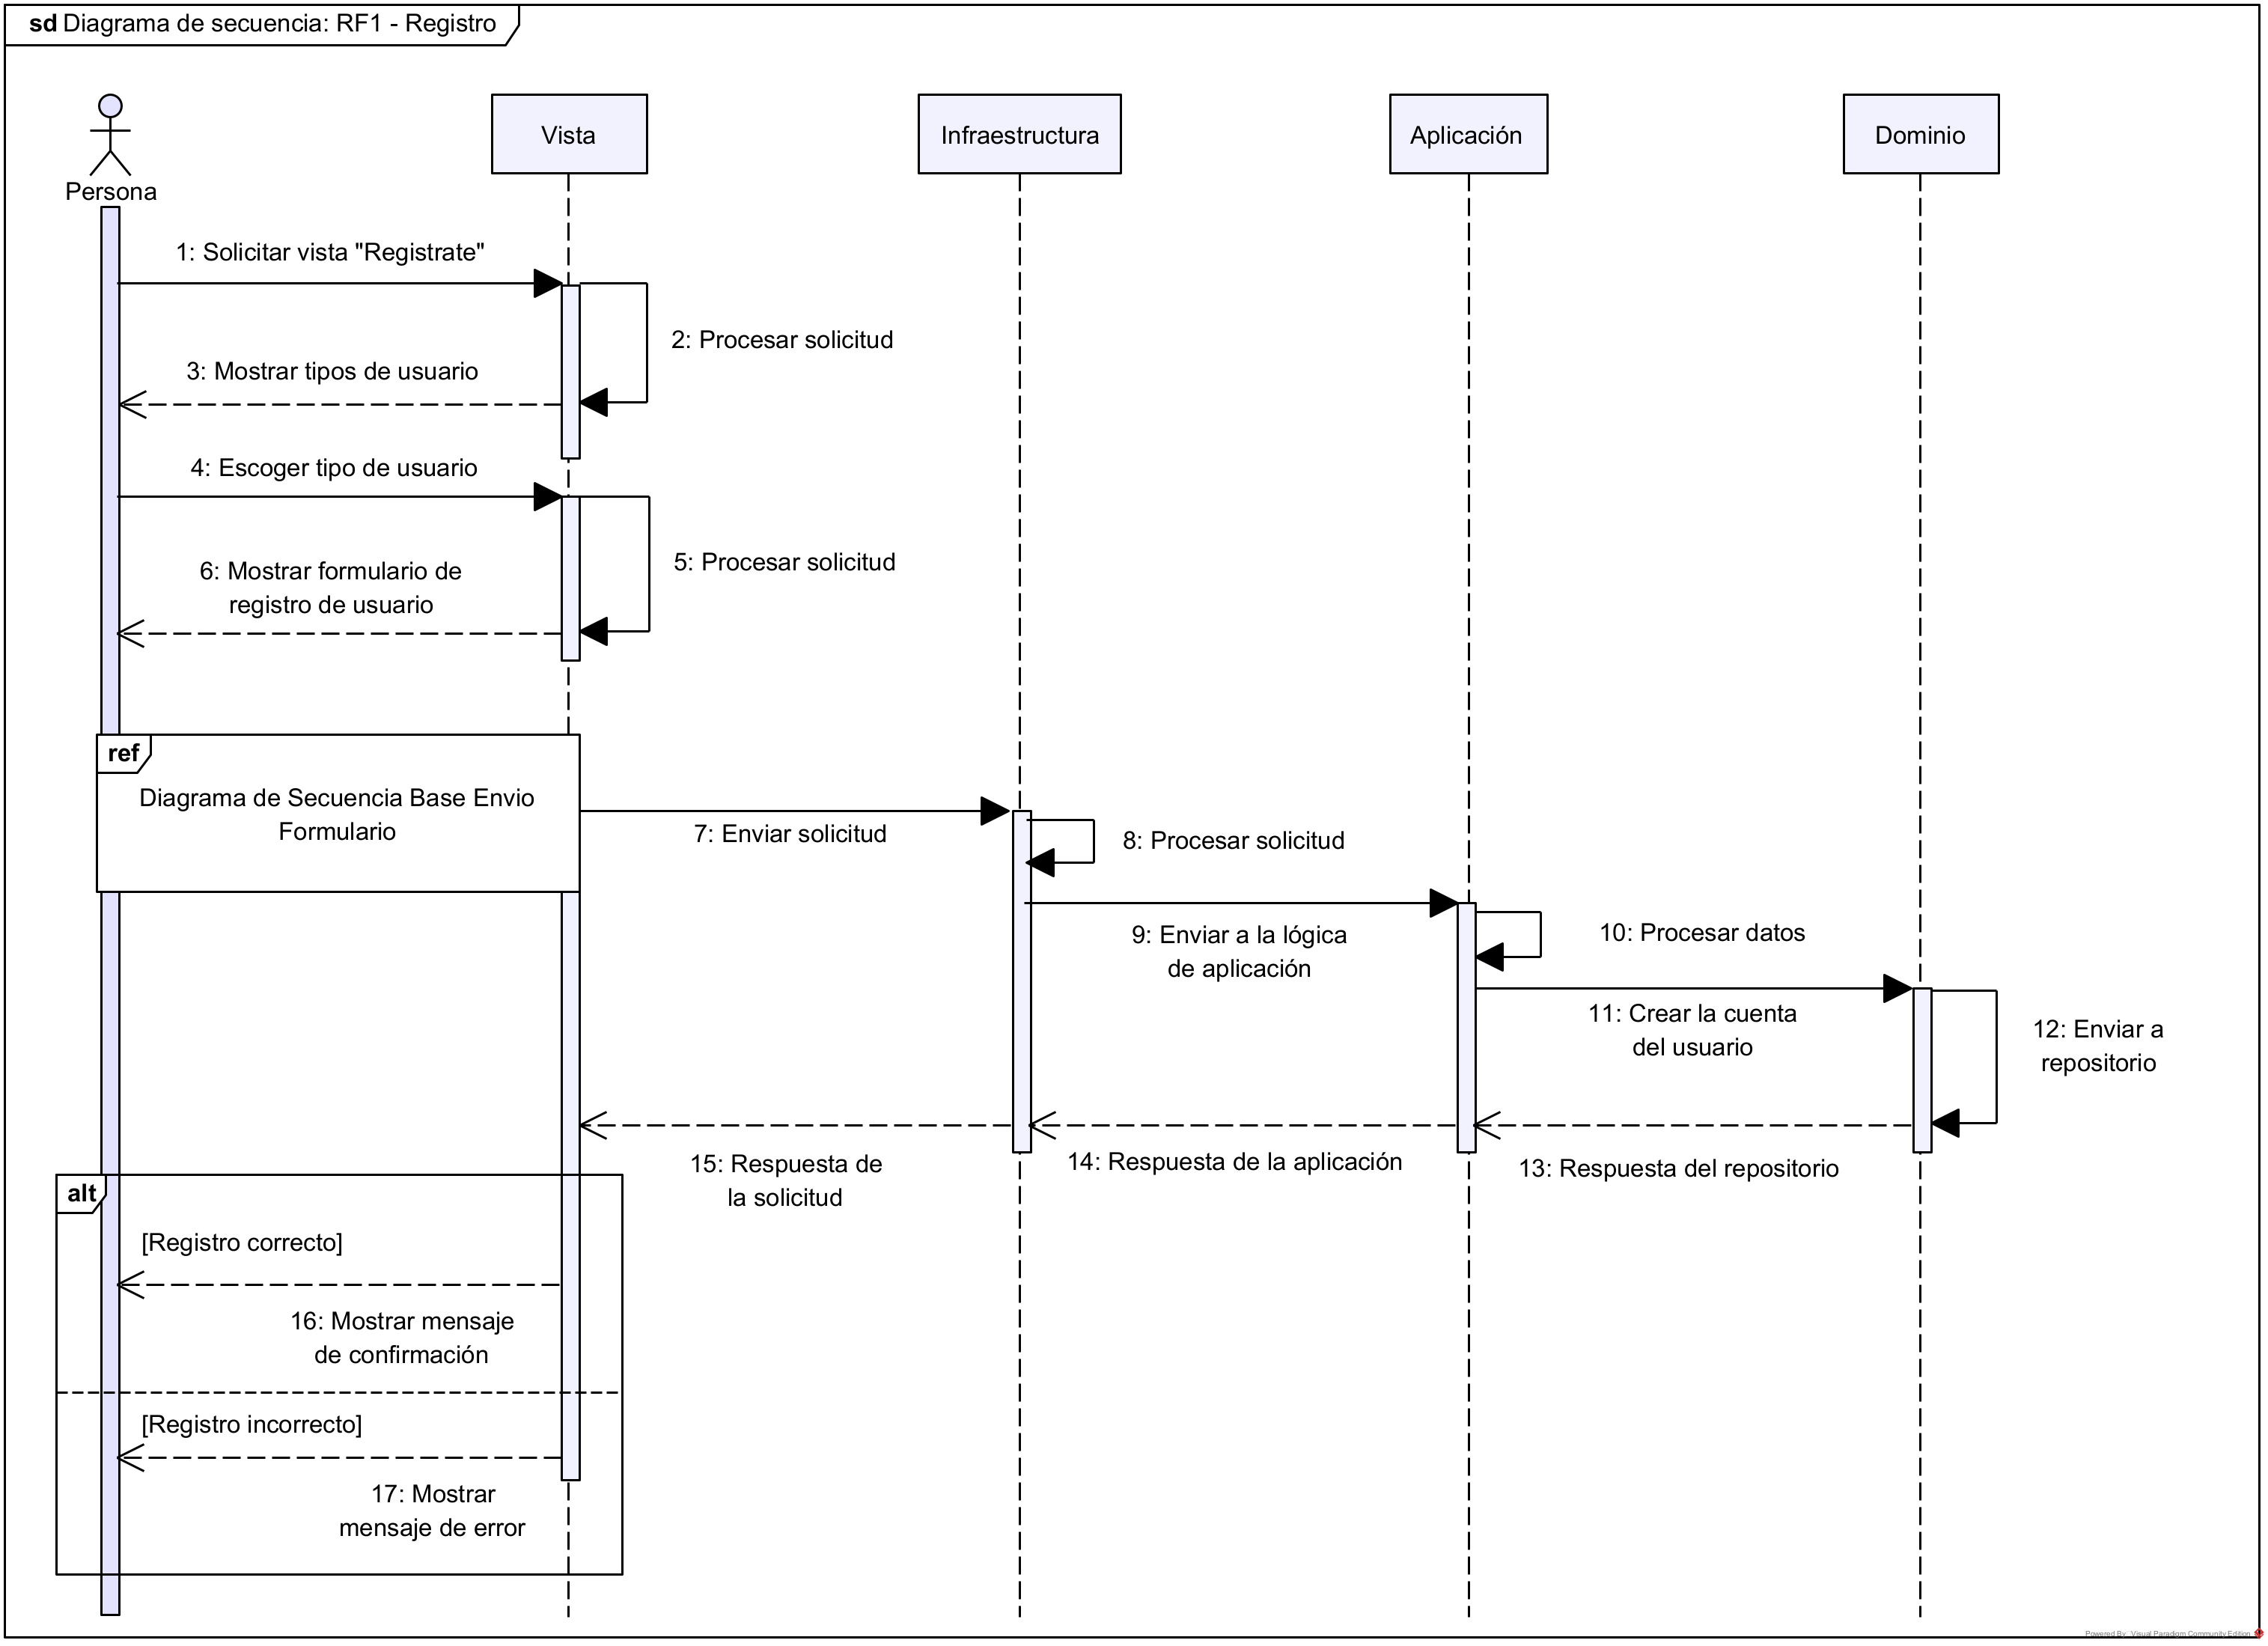
\includegraphics[width=0.8\textwidth]{UML/Secuencia/Diagrama de Secuencia RF1.0 Registro.png}
\end{figure}


\begin{figure}[H]
    \centering
    \caption{Diagrama de Secuencia para Solicitar Código (RF1.1).}
    \includegraphics[width=0.8\textwidth]{UML/Secuencia/Diagrama de Secuencia RF1.1 Solicitar Código.png}
\end{figure}


\begin{figure}[H]
	\centering
	\caption{Diagrama de Secuencia para Iniciar Sesión (RF2.0).}
	\includegraphics[width=0.8\textwidth]{UML/Secuencia/Diagrama de Secuencia RF2.0 Iniciar Sesión.png}
\end{figure}


\begin{figure}[H]
	\centering
	\caption{Diagrama de Secuencia para Cerrar Sesión (RF2.1).}
 \includegraphics[width=0.8\textwidth]{UML/Secuencia/Diagrama de Secuencia RF2.1 Cerrar Sesión.png}
\end{figure}


\begin{figure}[H]
	\centering
		\caption{Diagrama de Secuencia para Recuperar Contraseña (RF2.2).}
	\includegraphics[width=0.8\textwidth]{UML/Secuencia/Diagrama de Secuencia RF2.2 Recuperar Contraseña.png}
\end{figure}


\begin{figure}[H]
	\centering
		\caption{Diagrama de Secuencia para Crear Cámara (RF3.1).}
	\includegraphics[width=0.8\textwidth]{UML/Secuencia/Diagrama de Secuencia RF3.1 Crear Cámara.png}
\end{figure}


\begin{figure}[H]
	\centering
		\caption{Diagrama de Secuencia para Activar Cámara (RF3.1.1).}
	\includegraphics[width=0.63\textwidth]{UML/Secuencia/Diagrama de Secuencia RF3.1.1 Activar Cámara.png}
\end{figure}


\begin{figure}[H]
	\centering
	\caption{Diagrama de Secuencia para Activar Hardware (RF3.1.1).}
	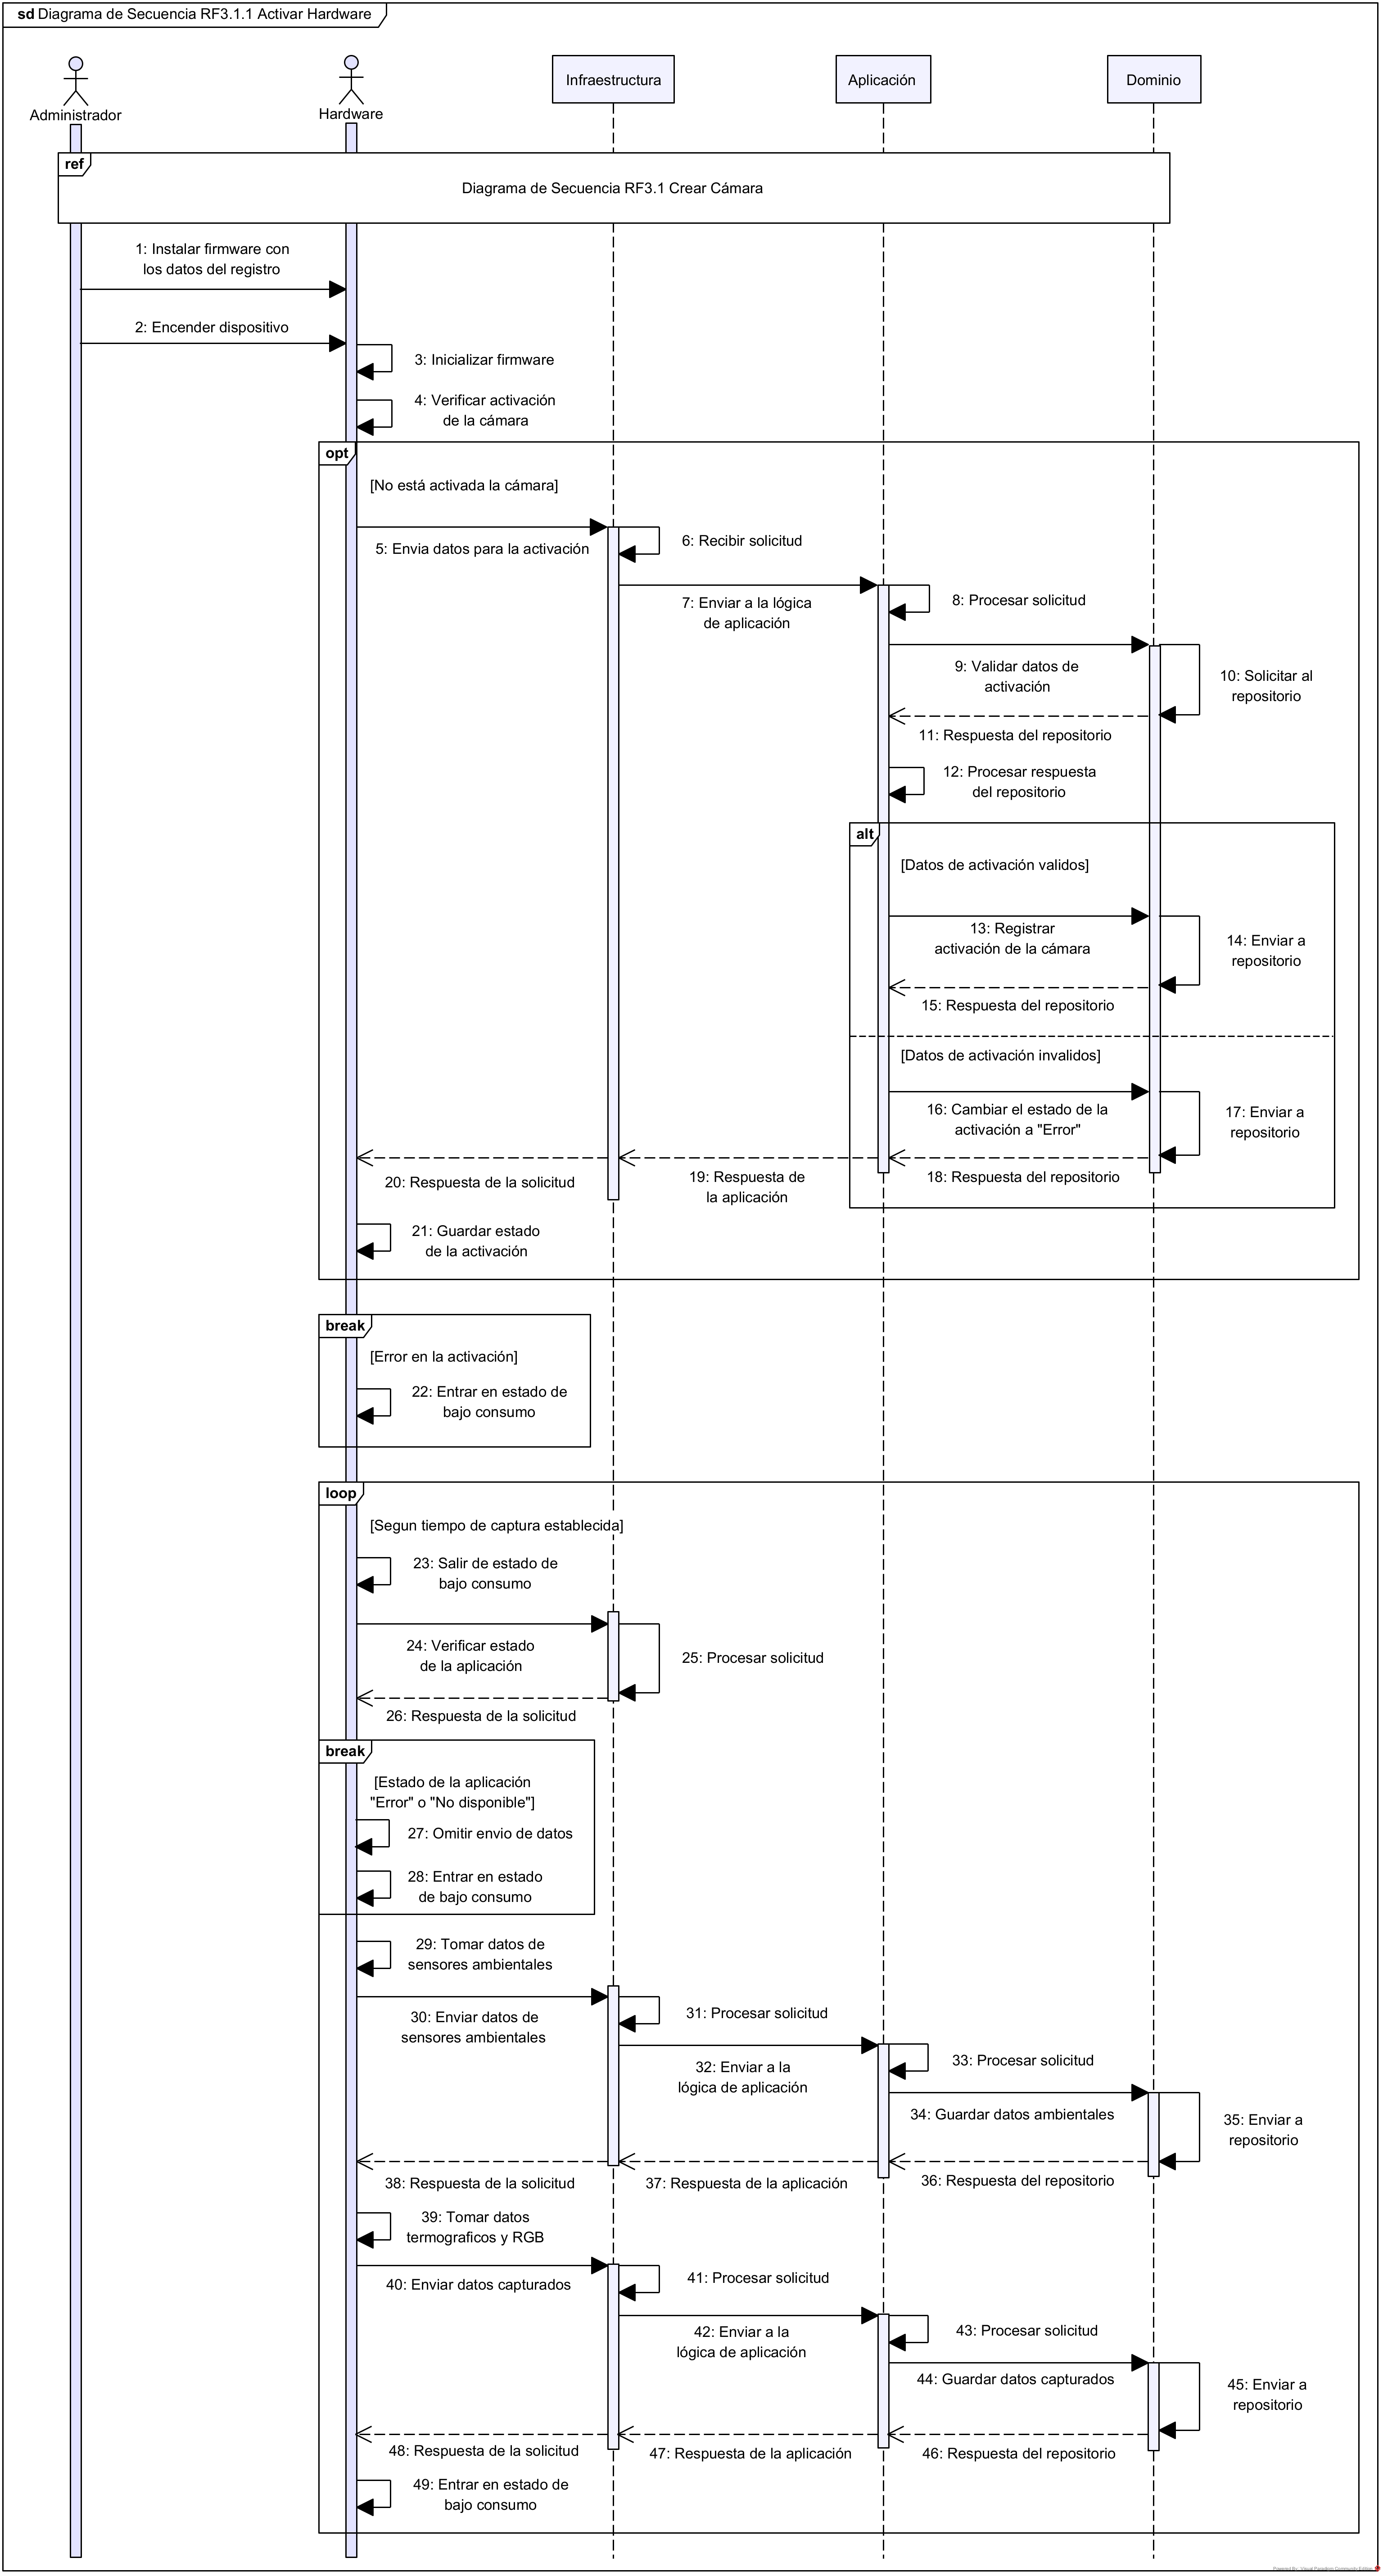
\includegraphics[width=0.6\textwidth]{UML/Secuencia/Diagrama de Secuencia RF3.1.1 Activar Hardware.png}
\end{figure}


\begin{figure}[H]
	\centering
		\caption{Diagrama de Secuencia para Consultar Cámara (RF3.2).}
	\includegraphics[width=0.8\textwidth]{UML/Secuencia/Diagrama de Secuencia RF3.2 Consultar Cámara.png}
\end{figure}


\begin{figure}[H]
	\centering
	\caption{Diagrama de Secuencia para Editar Cámara (RF3.3).}
 \includegraphics[width=0.8\textwidth]{UML/Secuencia/Diagrama de Secuencia RF3.3 Editar Cámara.png}
\end{figure}


\begin{figure}[H]
	\centering
		\caption{Diagrama de Secuencia para Eliminar Cámara (RF3.4).}
	\includegraphics[width=0.8\textwidth]{UML/Secuencia/Diagrama de Secuencia RF3.4 Eliminar Cámara.png}
\end{figure}


\begin{figure}[H]
	\centering
	\caption{Diagrama de Secuencia para Consultar Perfil (RF4.1).}
 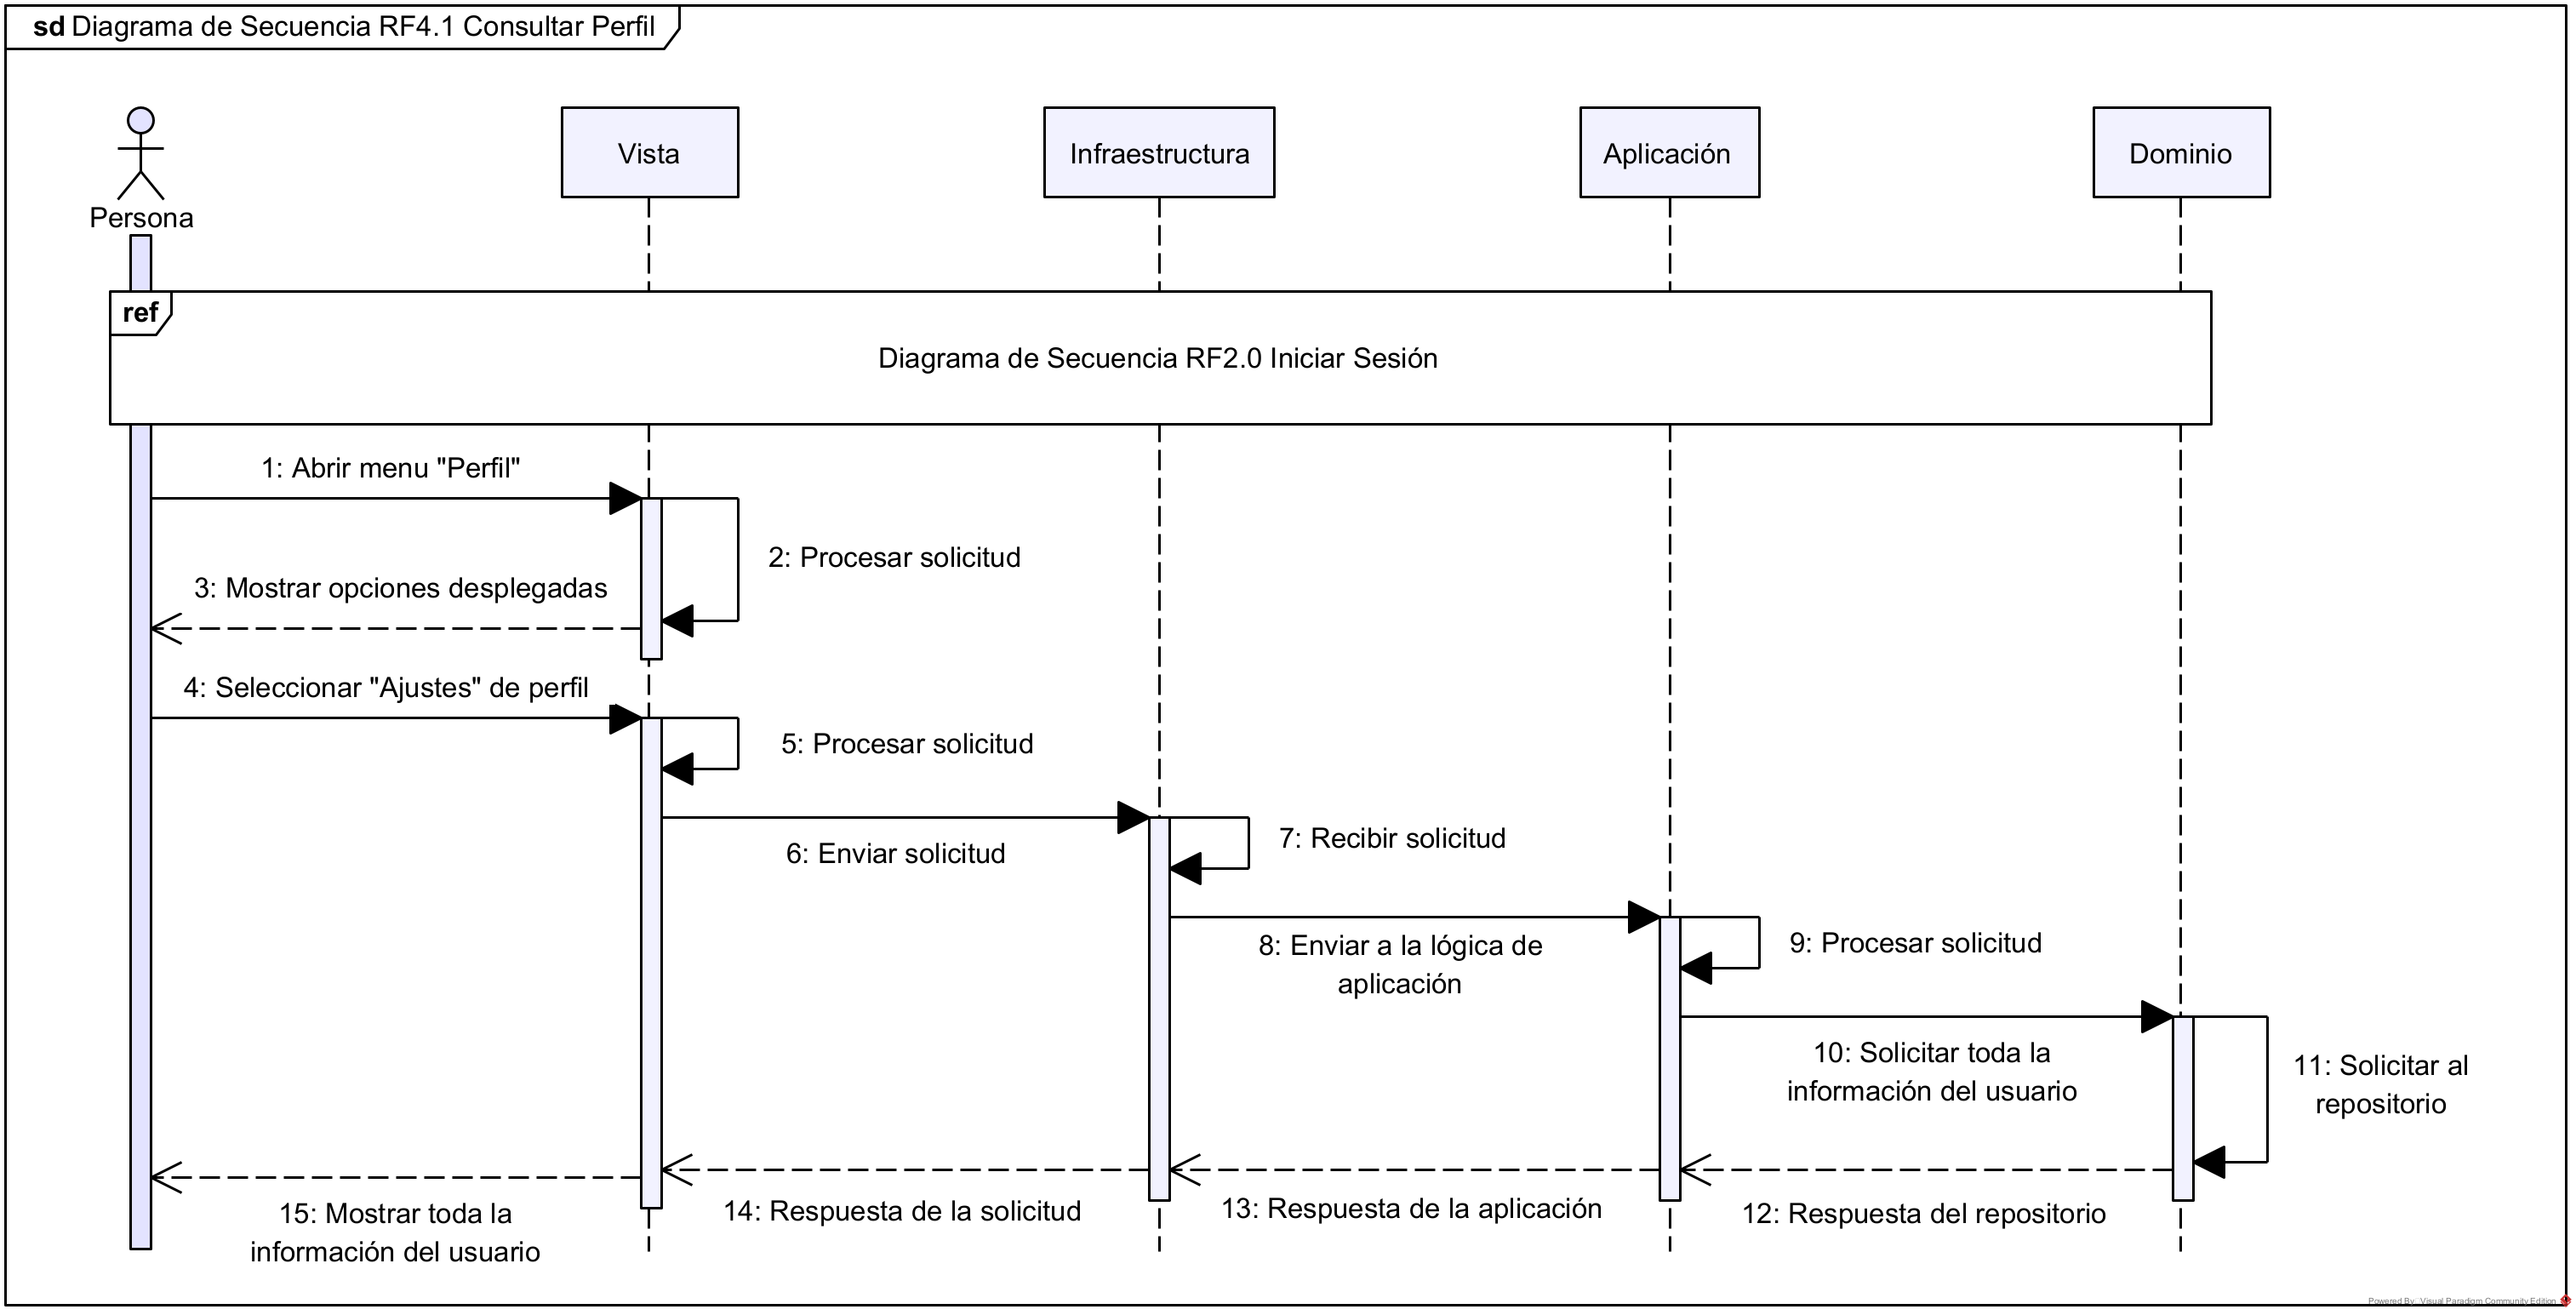
\includegraphics[width=0.8\textwidth]{UML/Secuencia/Diagrama de Secuencia RF4.1 Consultar Perfil.png}
\end{figure}


\begin{figure}[H]
	\centering
		\caption{Diagrama de Secuencia para Editar Perfil (RF4.2).}
	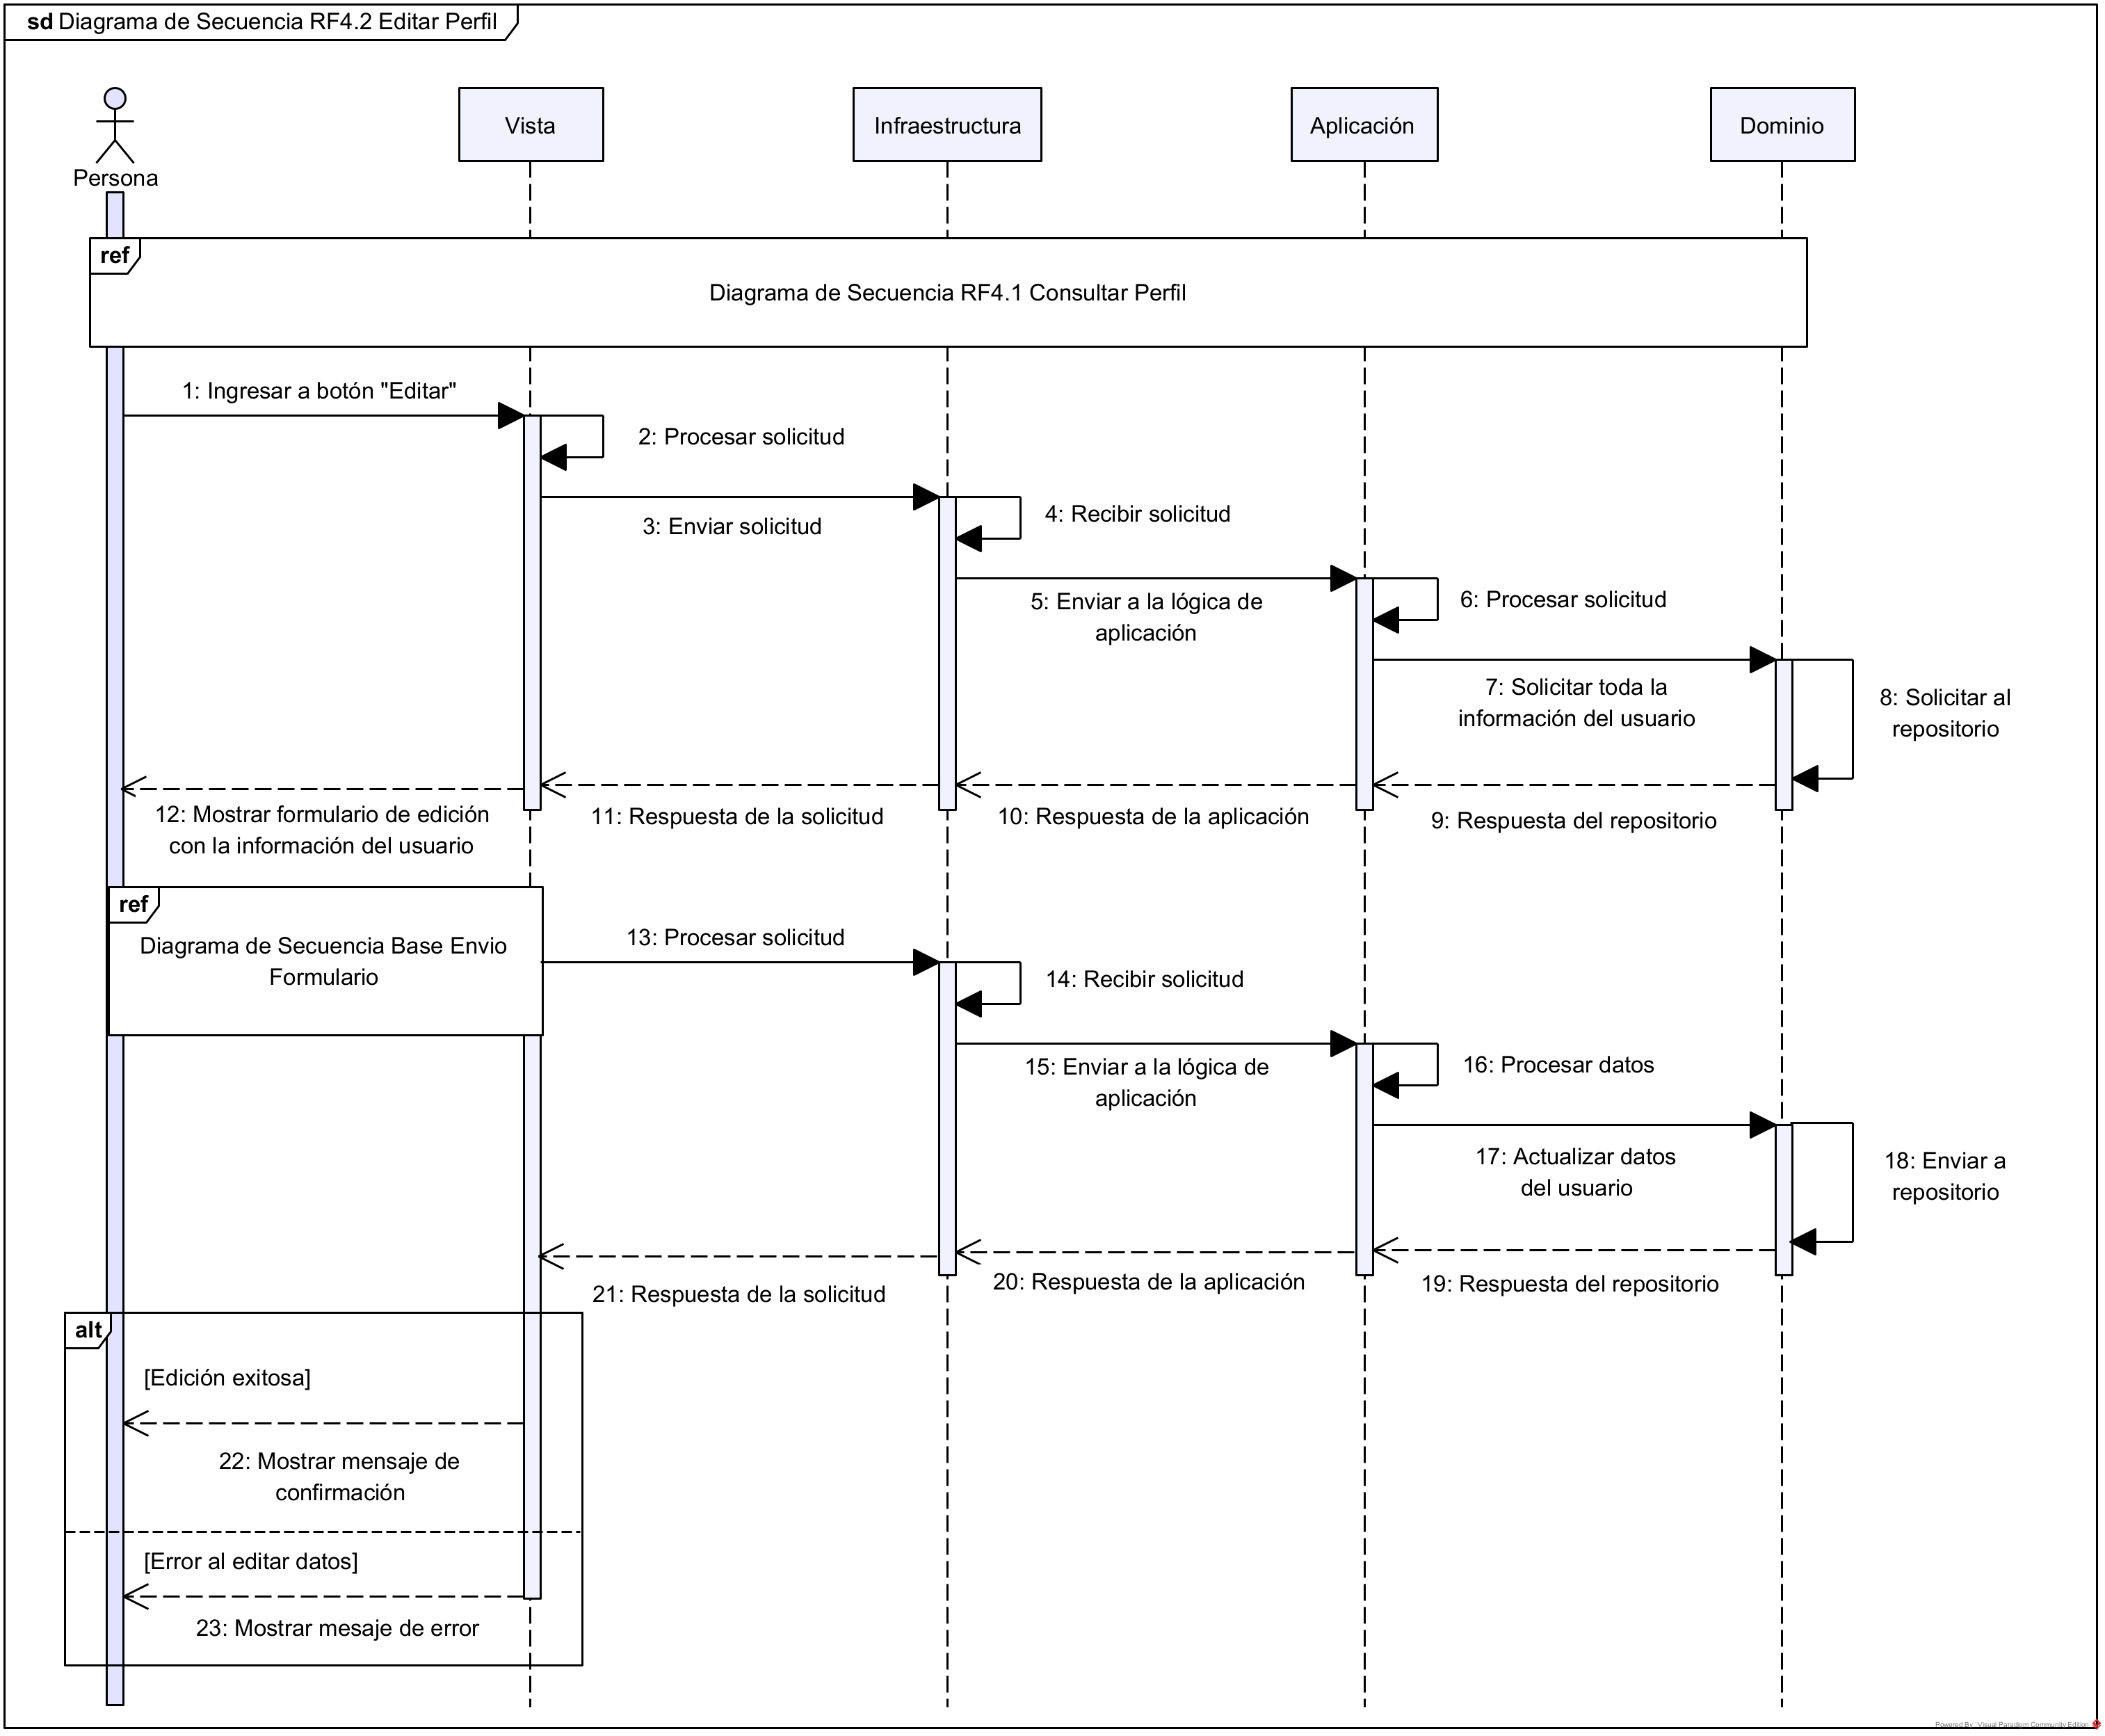
\includegraphics[width=0.8\textwidth]{UML/Secuencia/Diagrama de Secuencia RF4.2 Editar Perfil.png}
\end{figure}


\begin{figure}[H]
	\centering
	\caption{Diagrama de Secuencia para Eliminar Perfil (RF4.3).}
 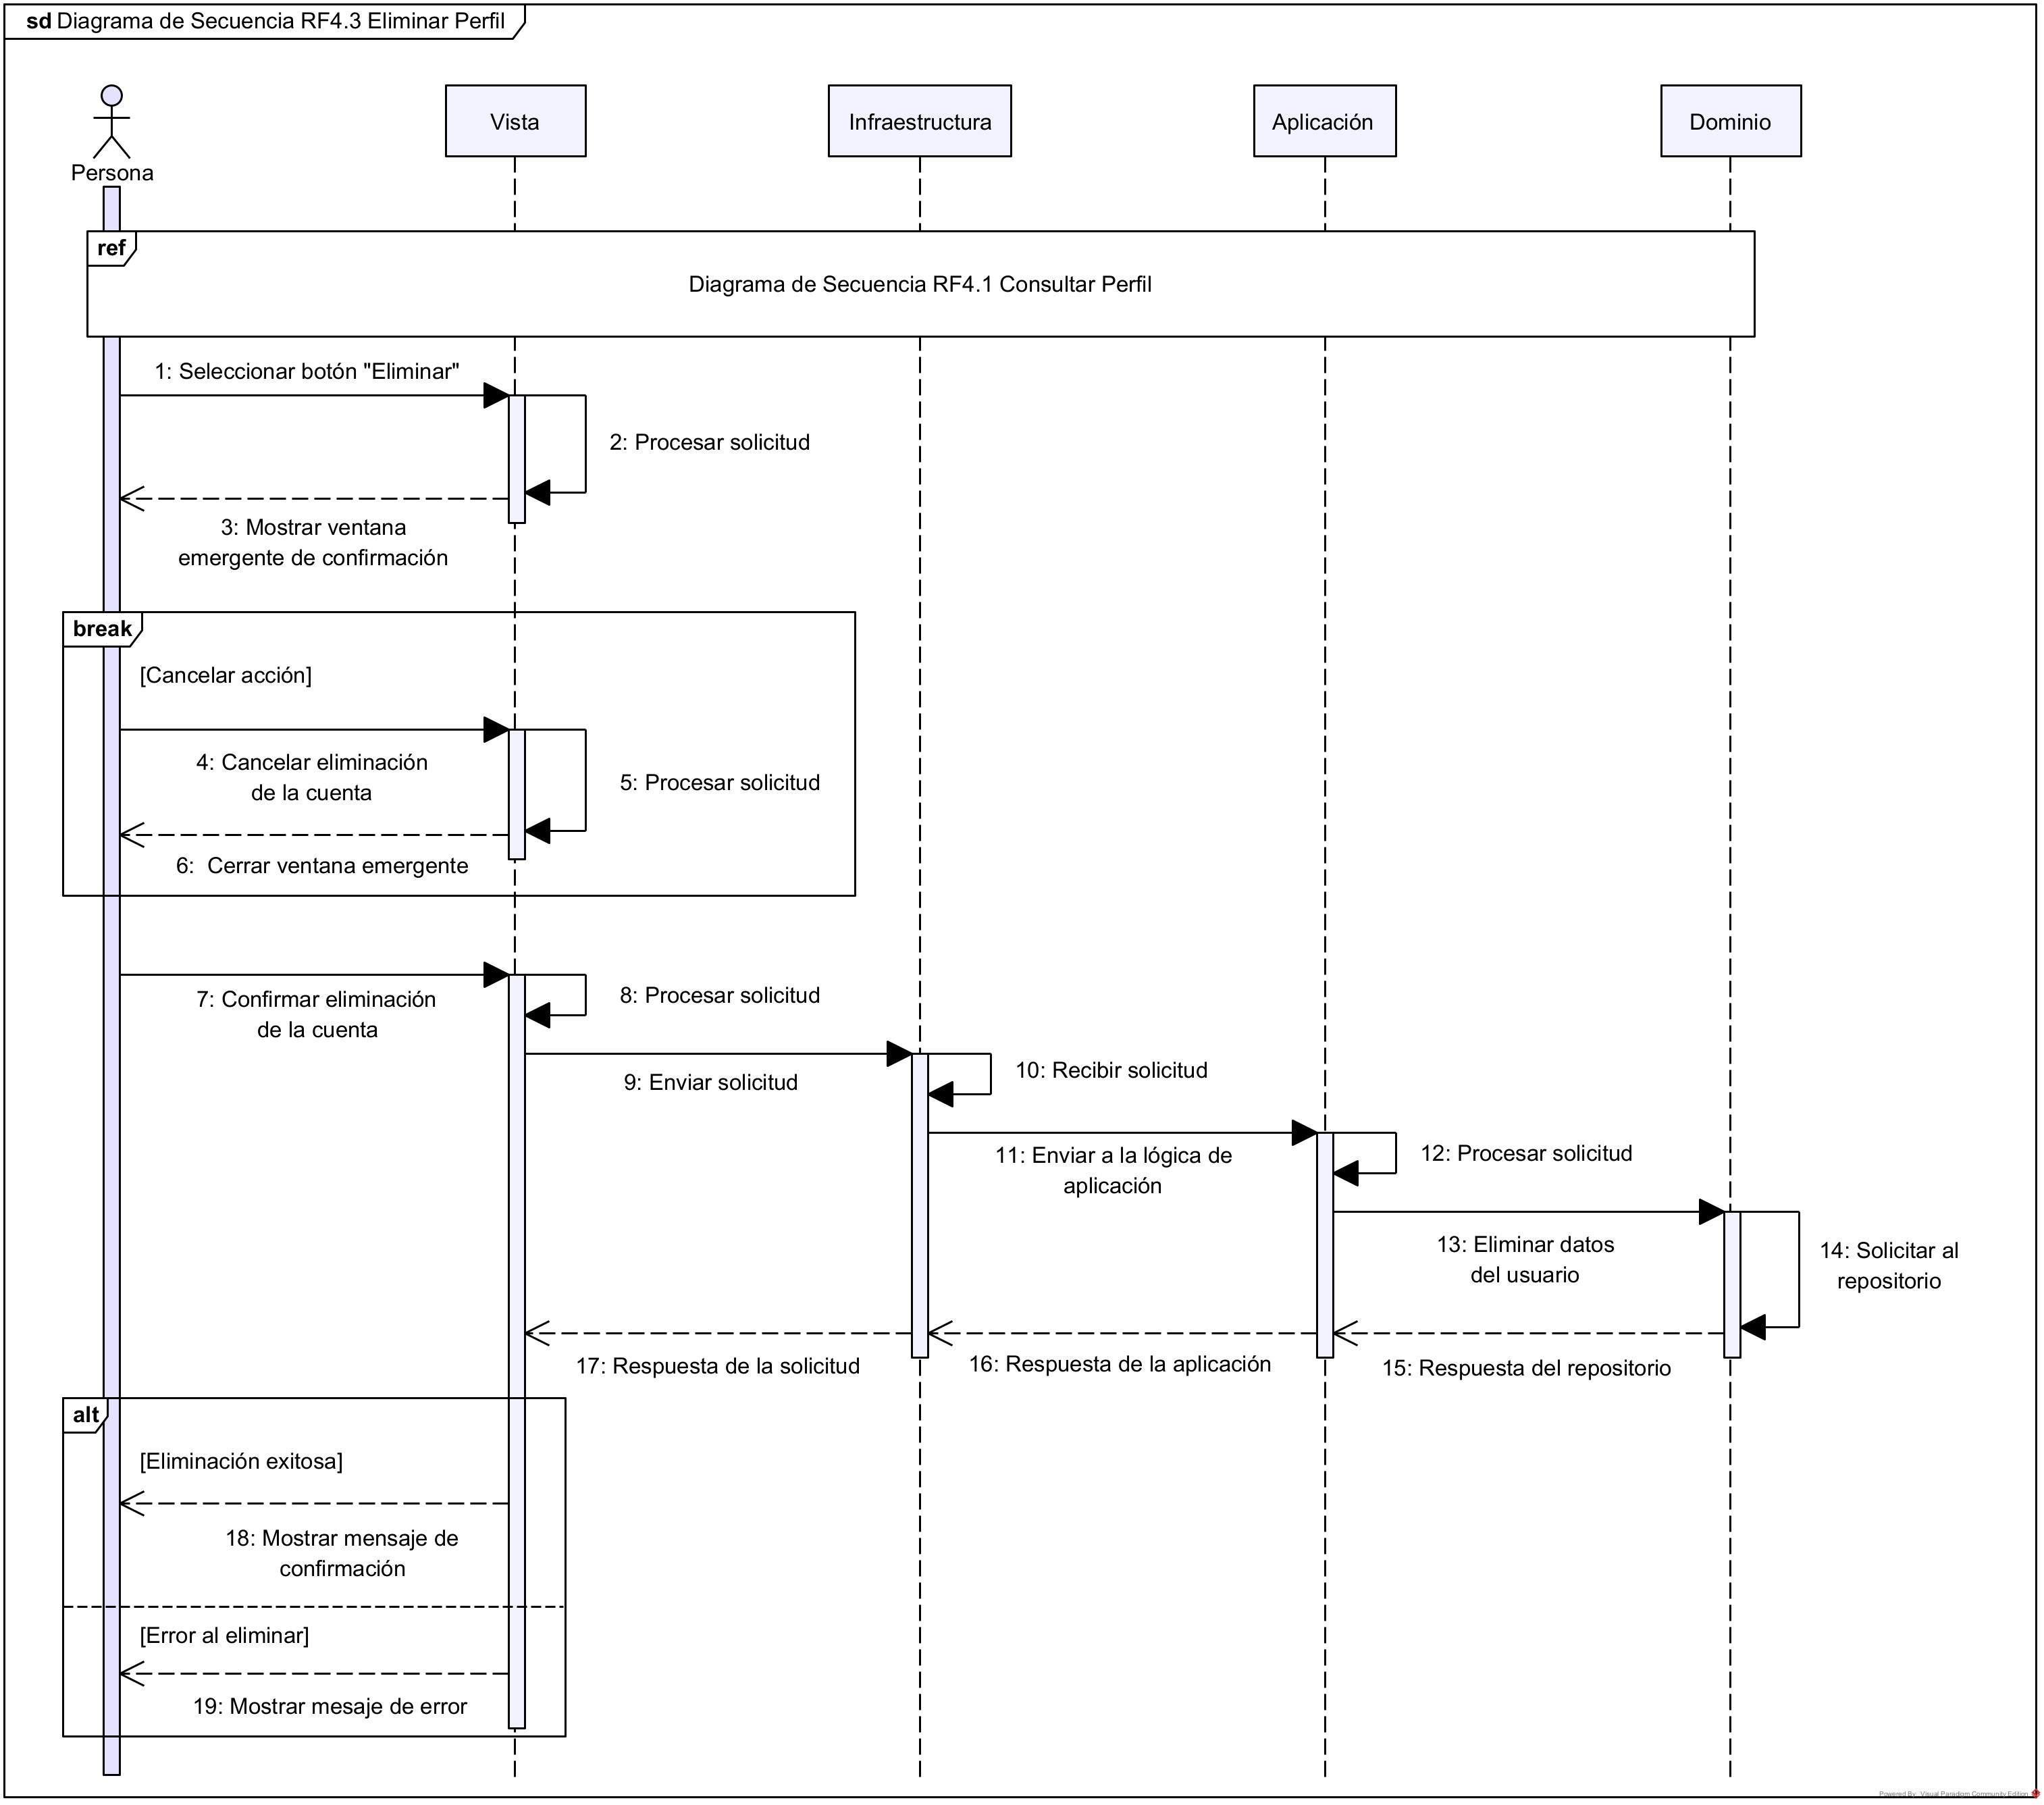
\includegraphics[width=0.8\textwidth]{UML/Secuencia/Diagrama de Secuencia RF4.3 Eliminar Perfil.png}
\end{figure}


\begin{figure}[H]
	\centering
		\caption{Diagrama de Secuencia para Cambiar Contraseña (RF4.4).}
	\includegraphics[width=0.8\textwidth]{UML/Secuencia/Diagrama de Secuencia RF4.4 Cambiar Contraseña.png}
\end{figure}


\begin{figure}[H]
	\centering
		\caption{Diagrama de Secuencia para Agregar Integrante de Cultivo (RF4.5).}
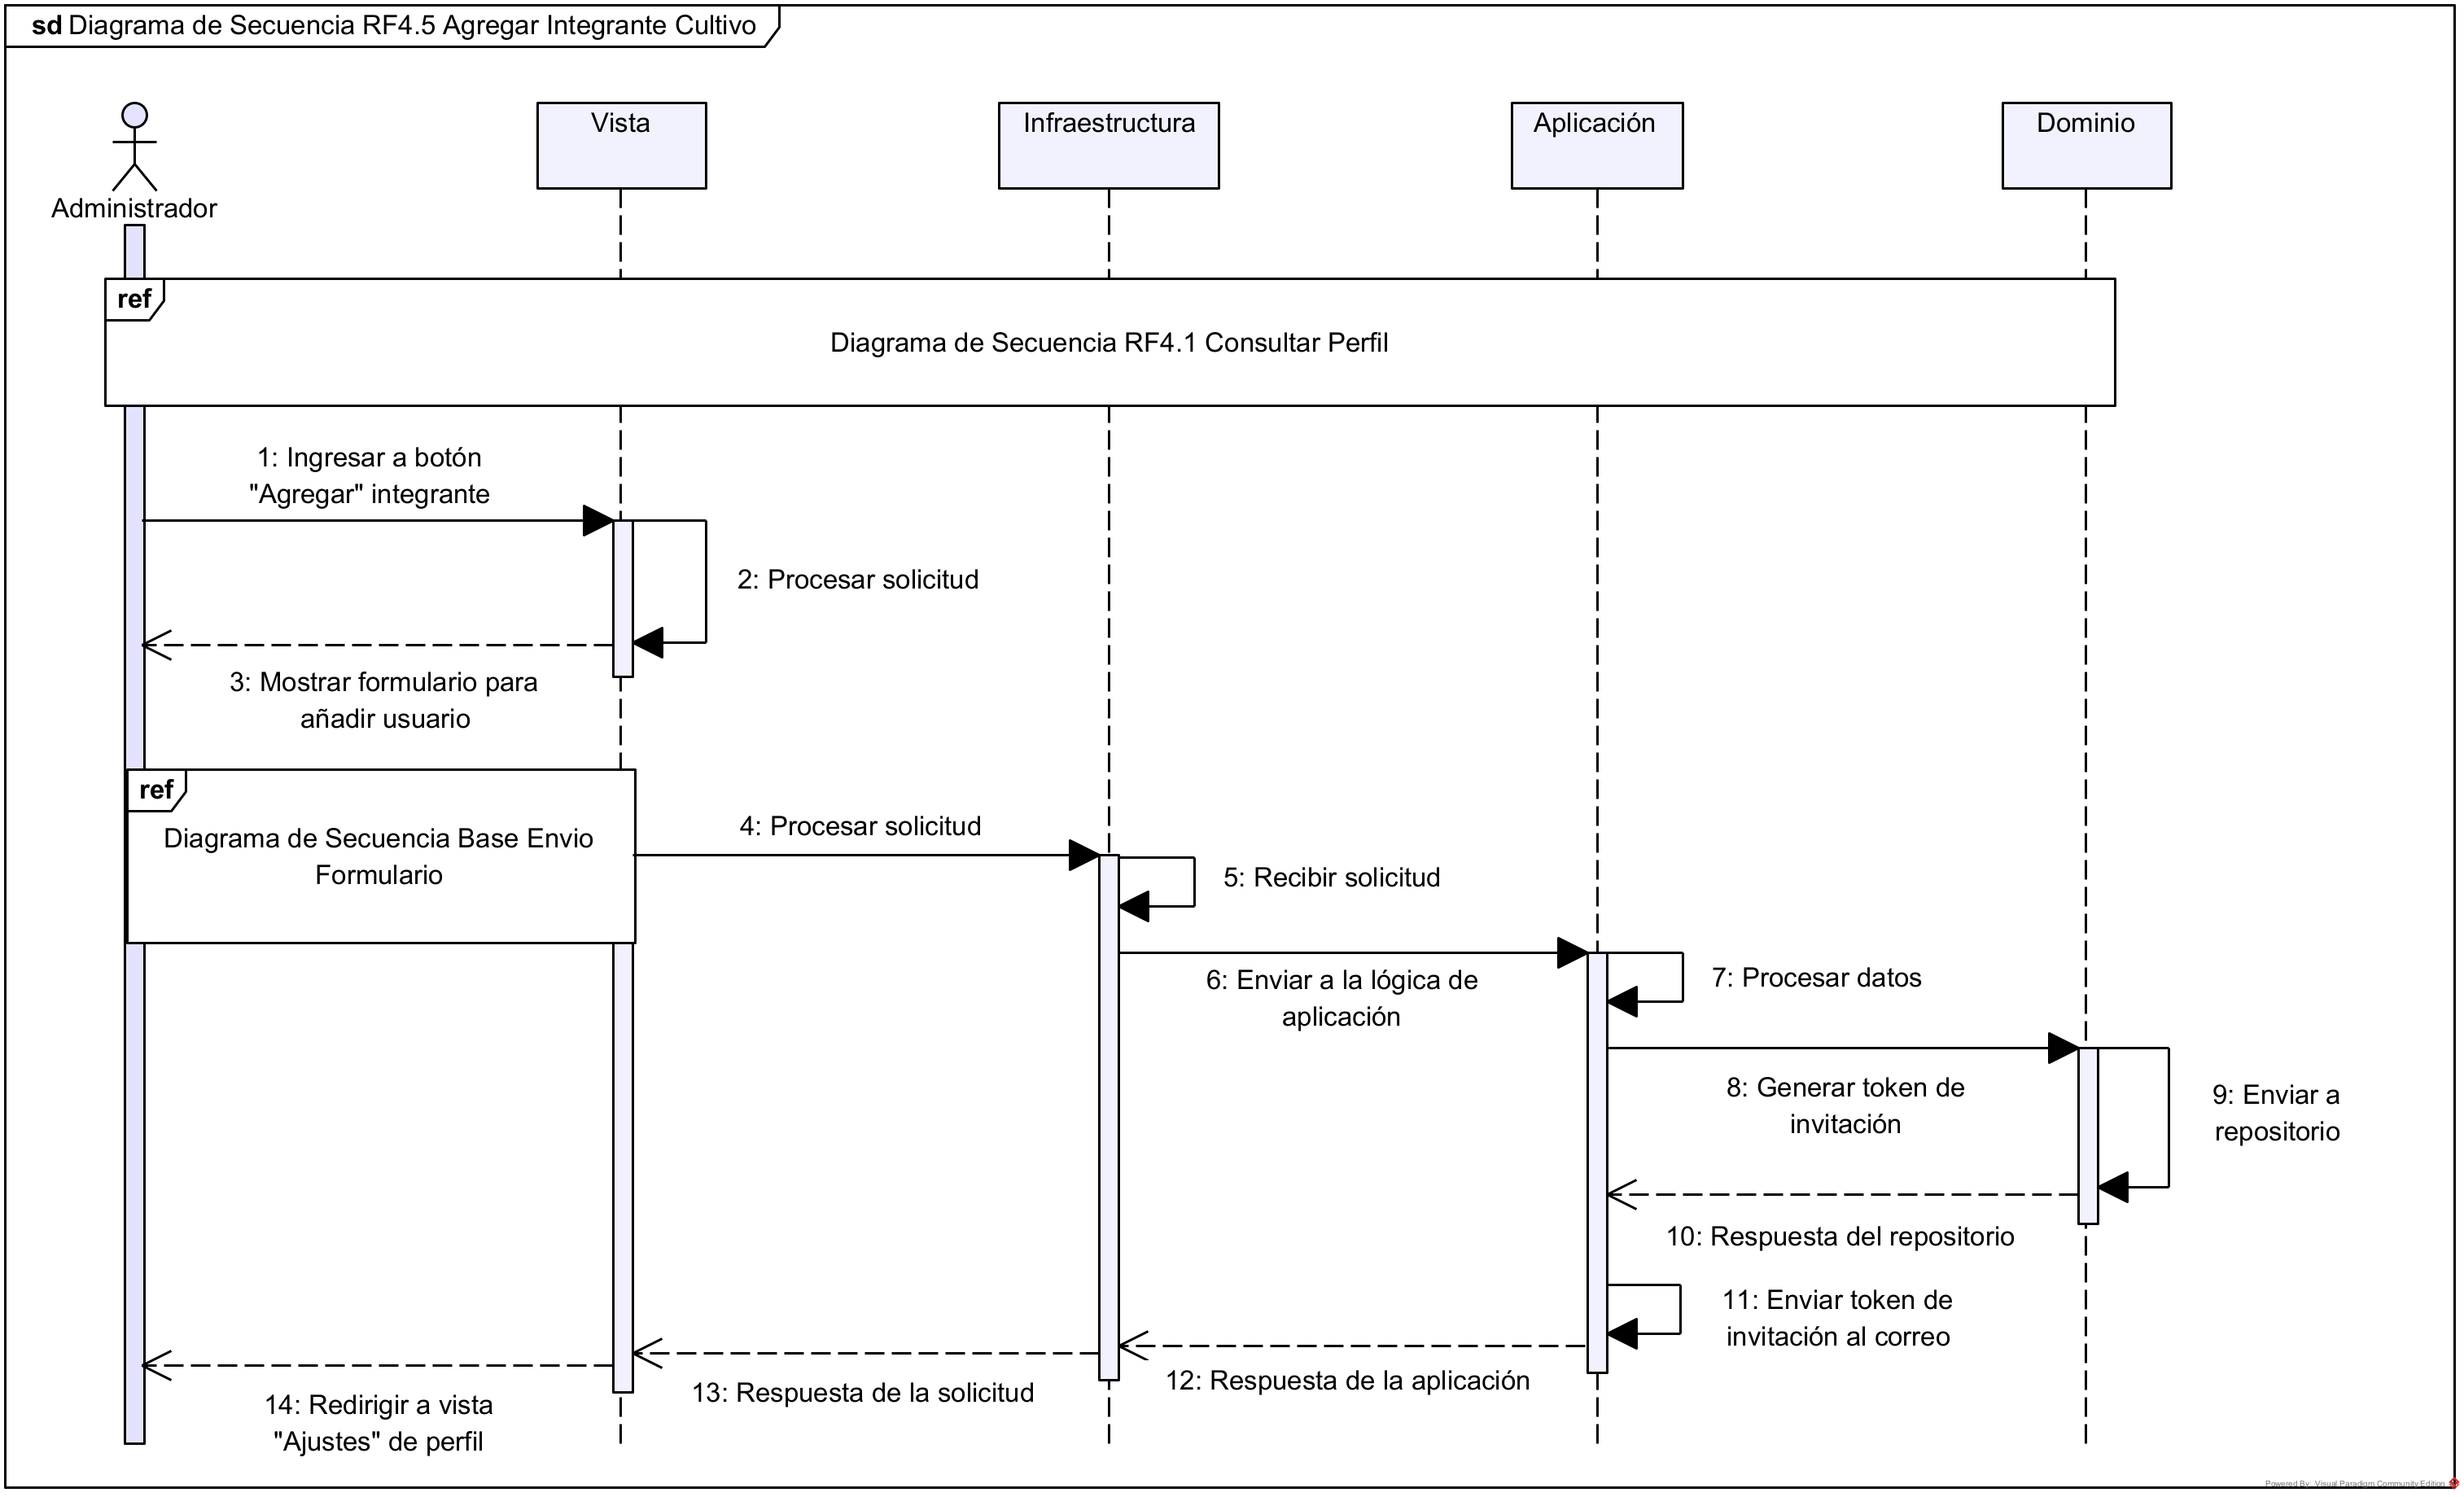
\includegraphics[width=0.8\textwidth]{UML/Secuencia/Diagrama de Secuencia RF4.5 Agregar Integrante Cultivo.png}
\end{figure}

\begin{figure}[H]
	\centering
	\caption{Diagrama de Secuencia para Eliminar Integrante de Cultivo (RF4.6).}
 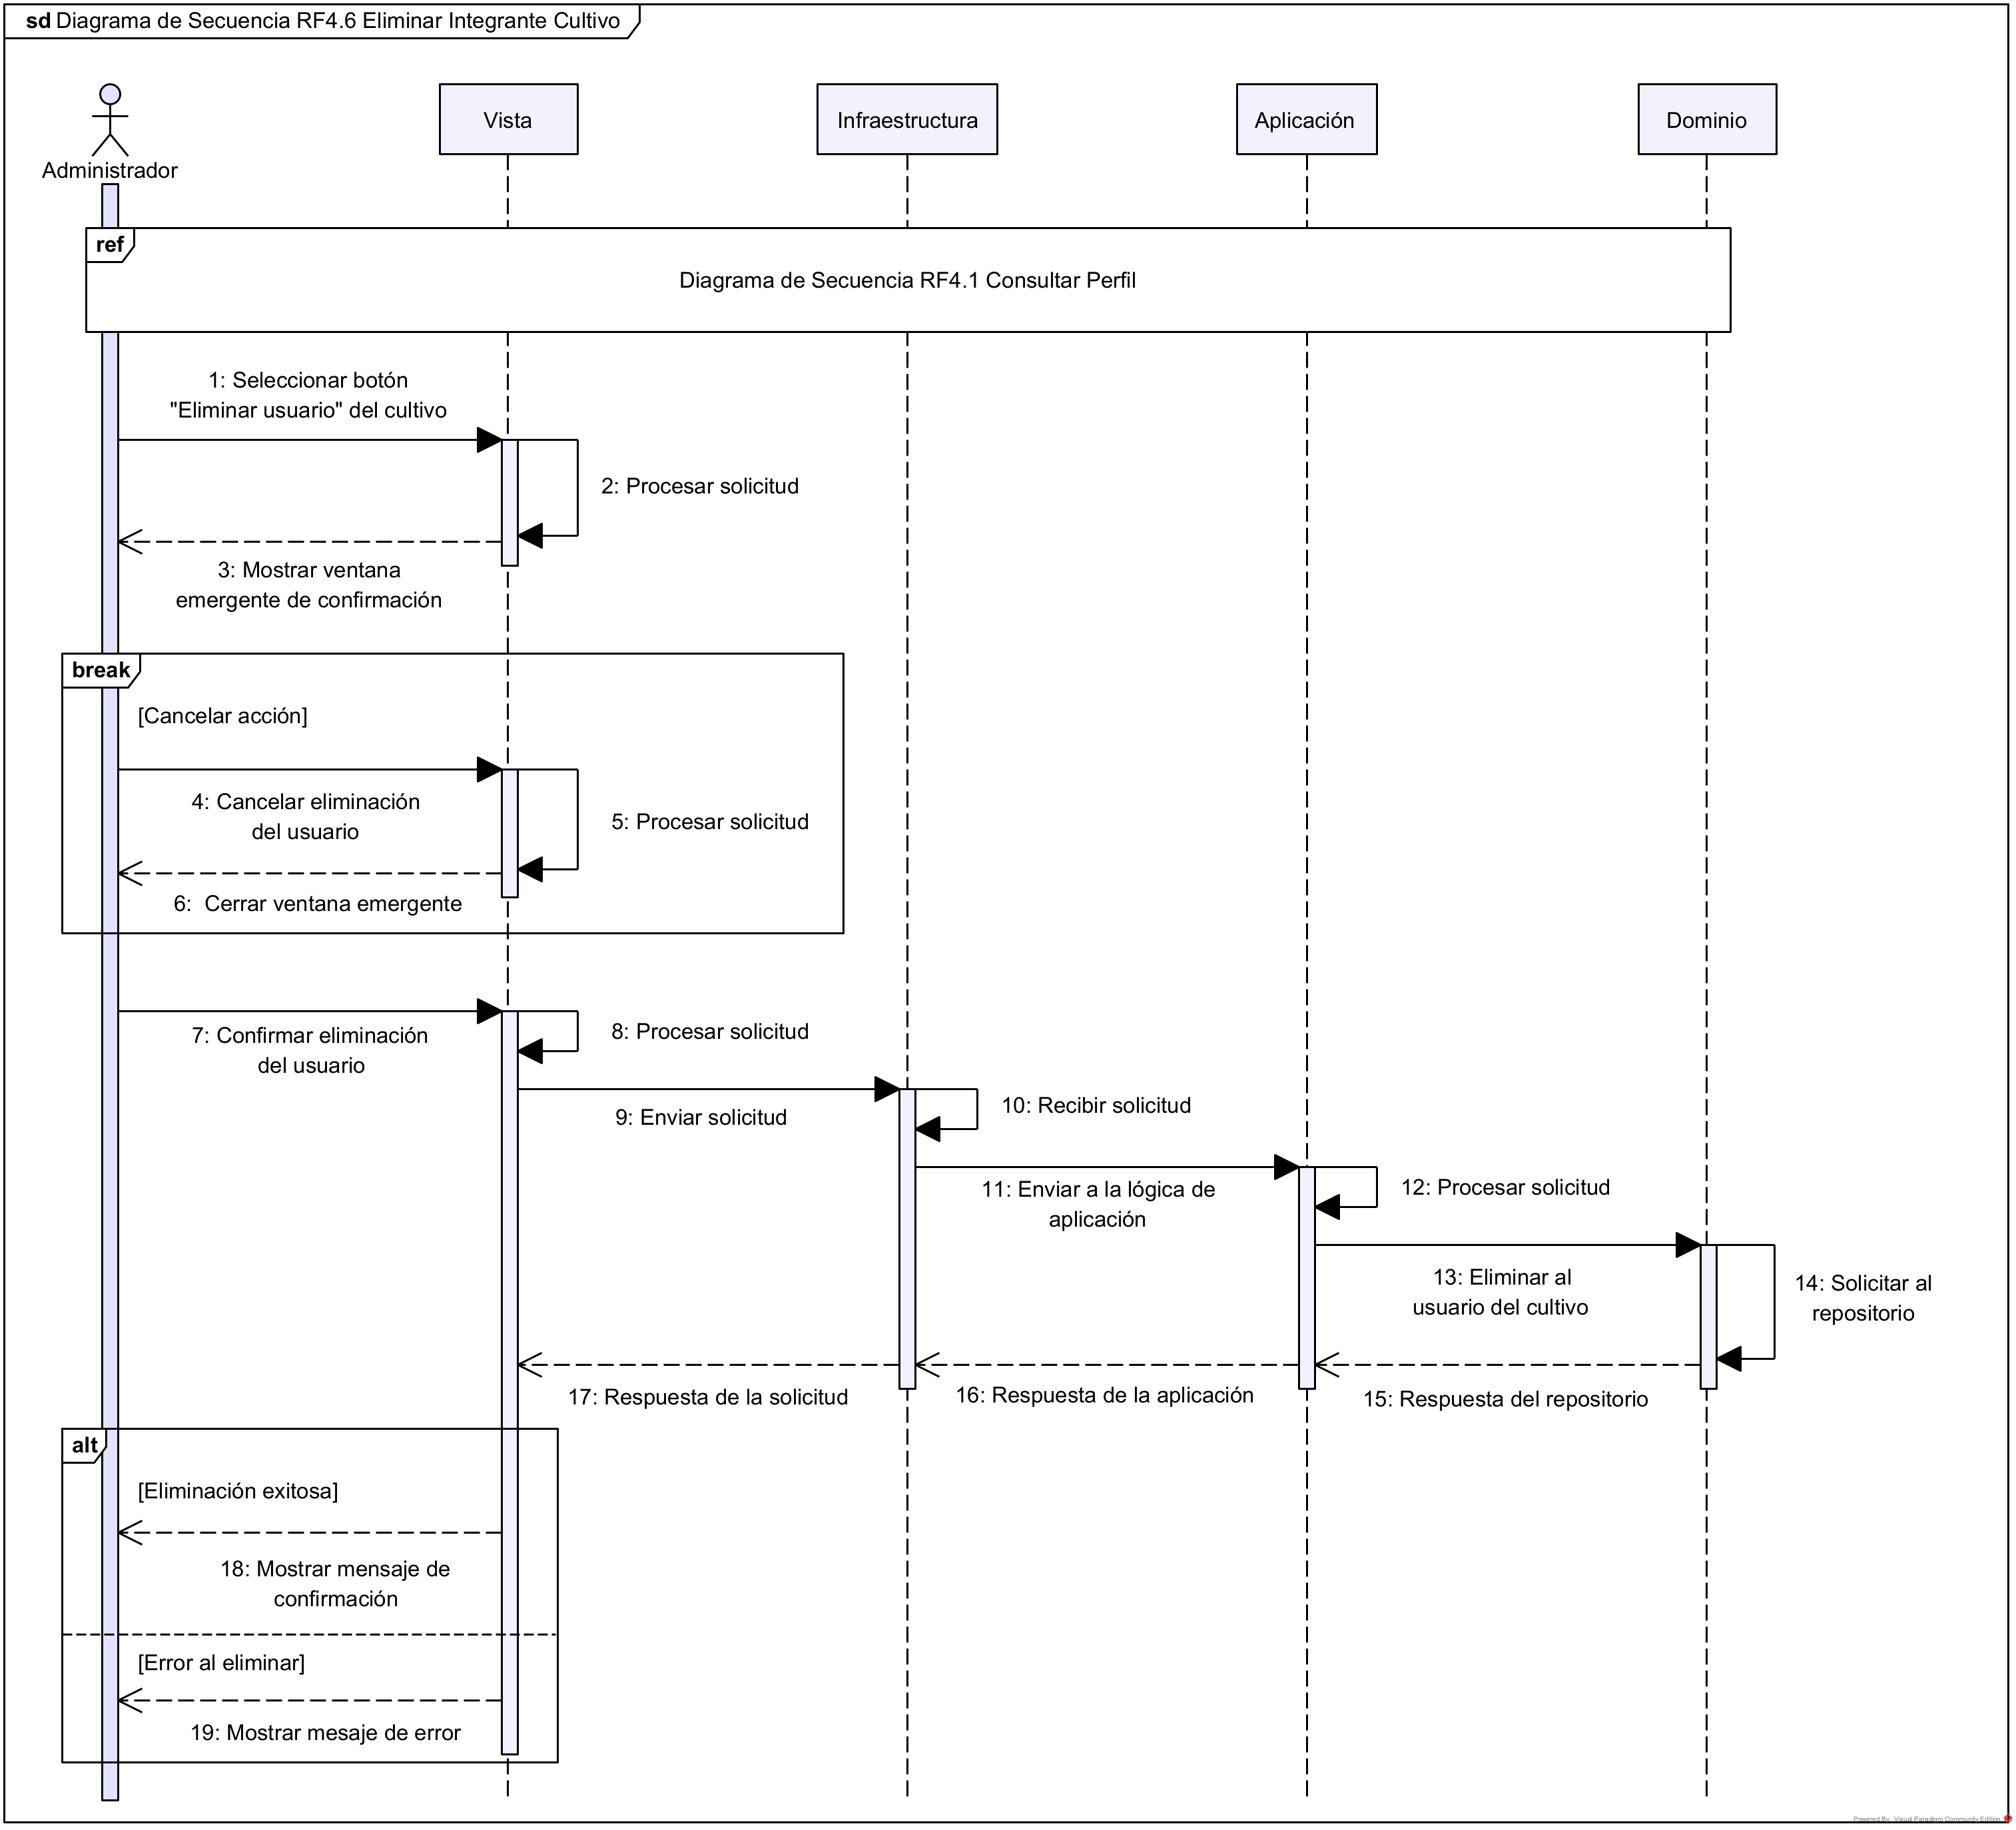
\includegraphics[width=0.8\textwidth]{UML/Secuencia/Diagrama de Secuencia RF4.6 Eliminar Integrante Cultivo.png}
\end{figure}


\begin{figure}[H]
	\centering
		\caption{Diagrama de Secuencia para el Módulo de Mediciones (RF5.0).}
	\includegraphics[width=0.8\textwidth]{UML/Secuencia/Diagrama de Secuencia RF5.0 Módulo de mediciones.png}
\end{figure}


\begin{figure}[H]
	\centering
	\caption{Diagrama de Secuencia para Crear Planta (RF6.1).}
 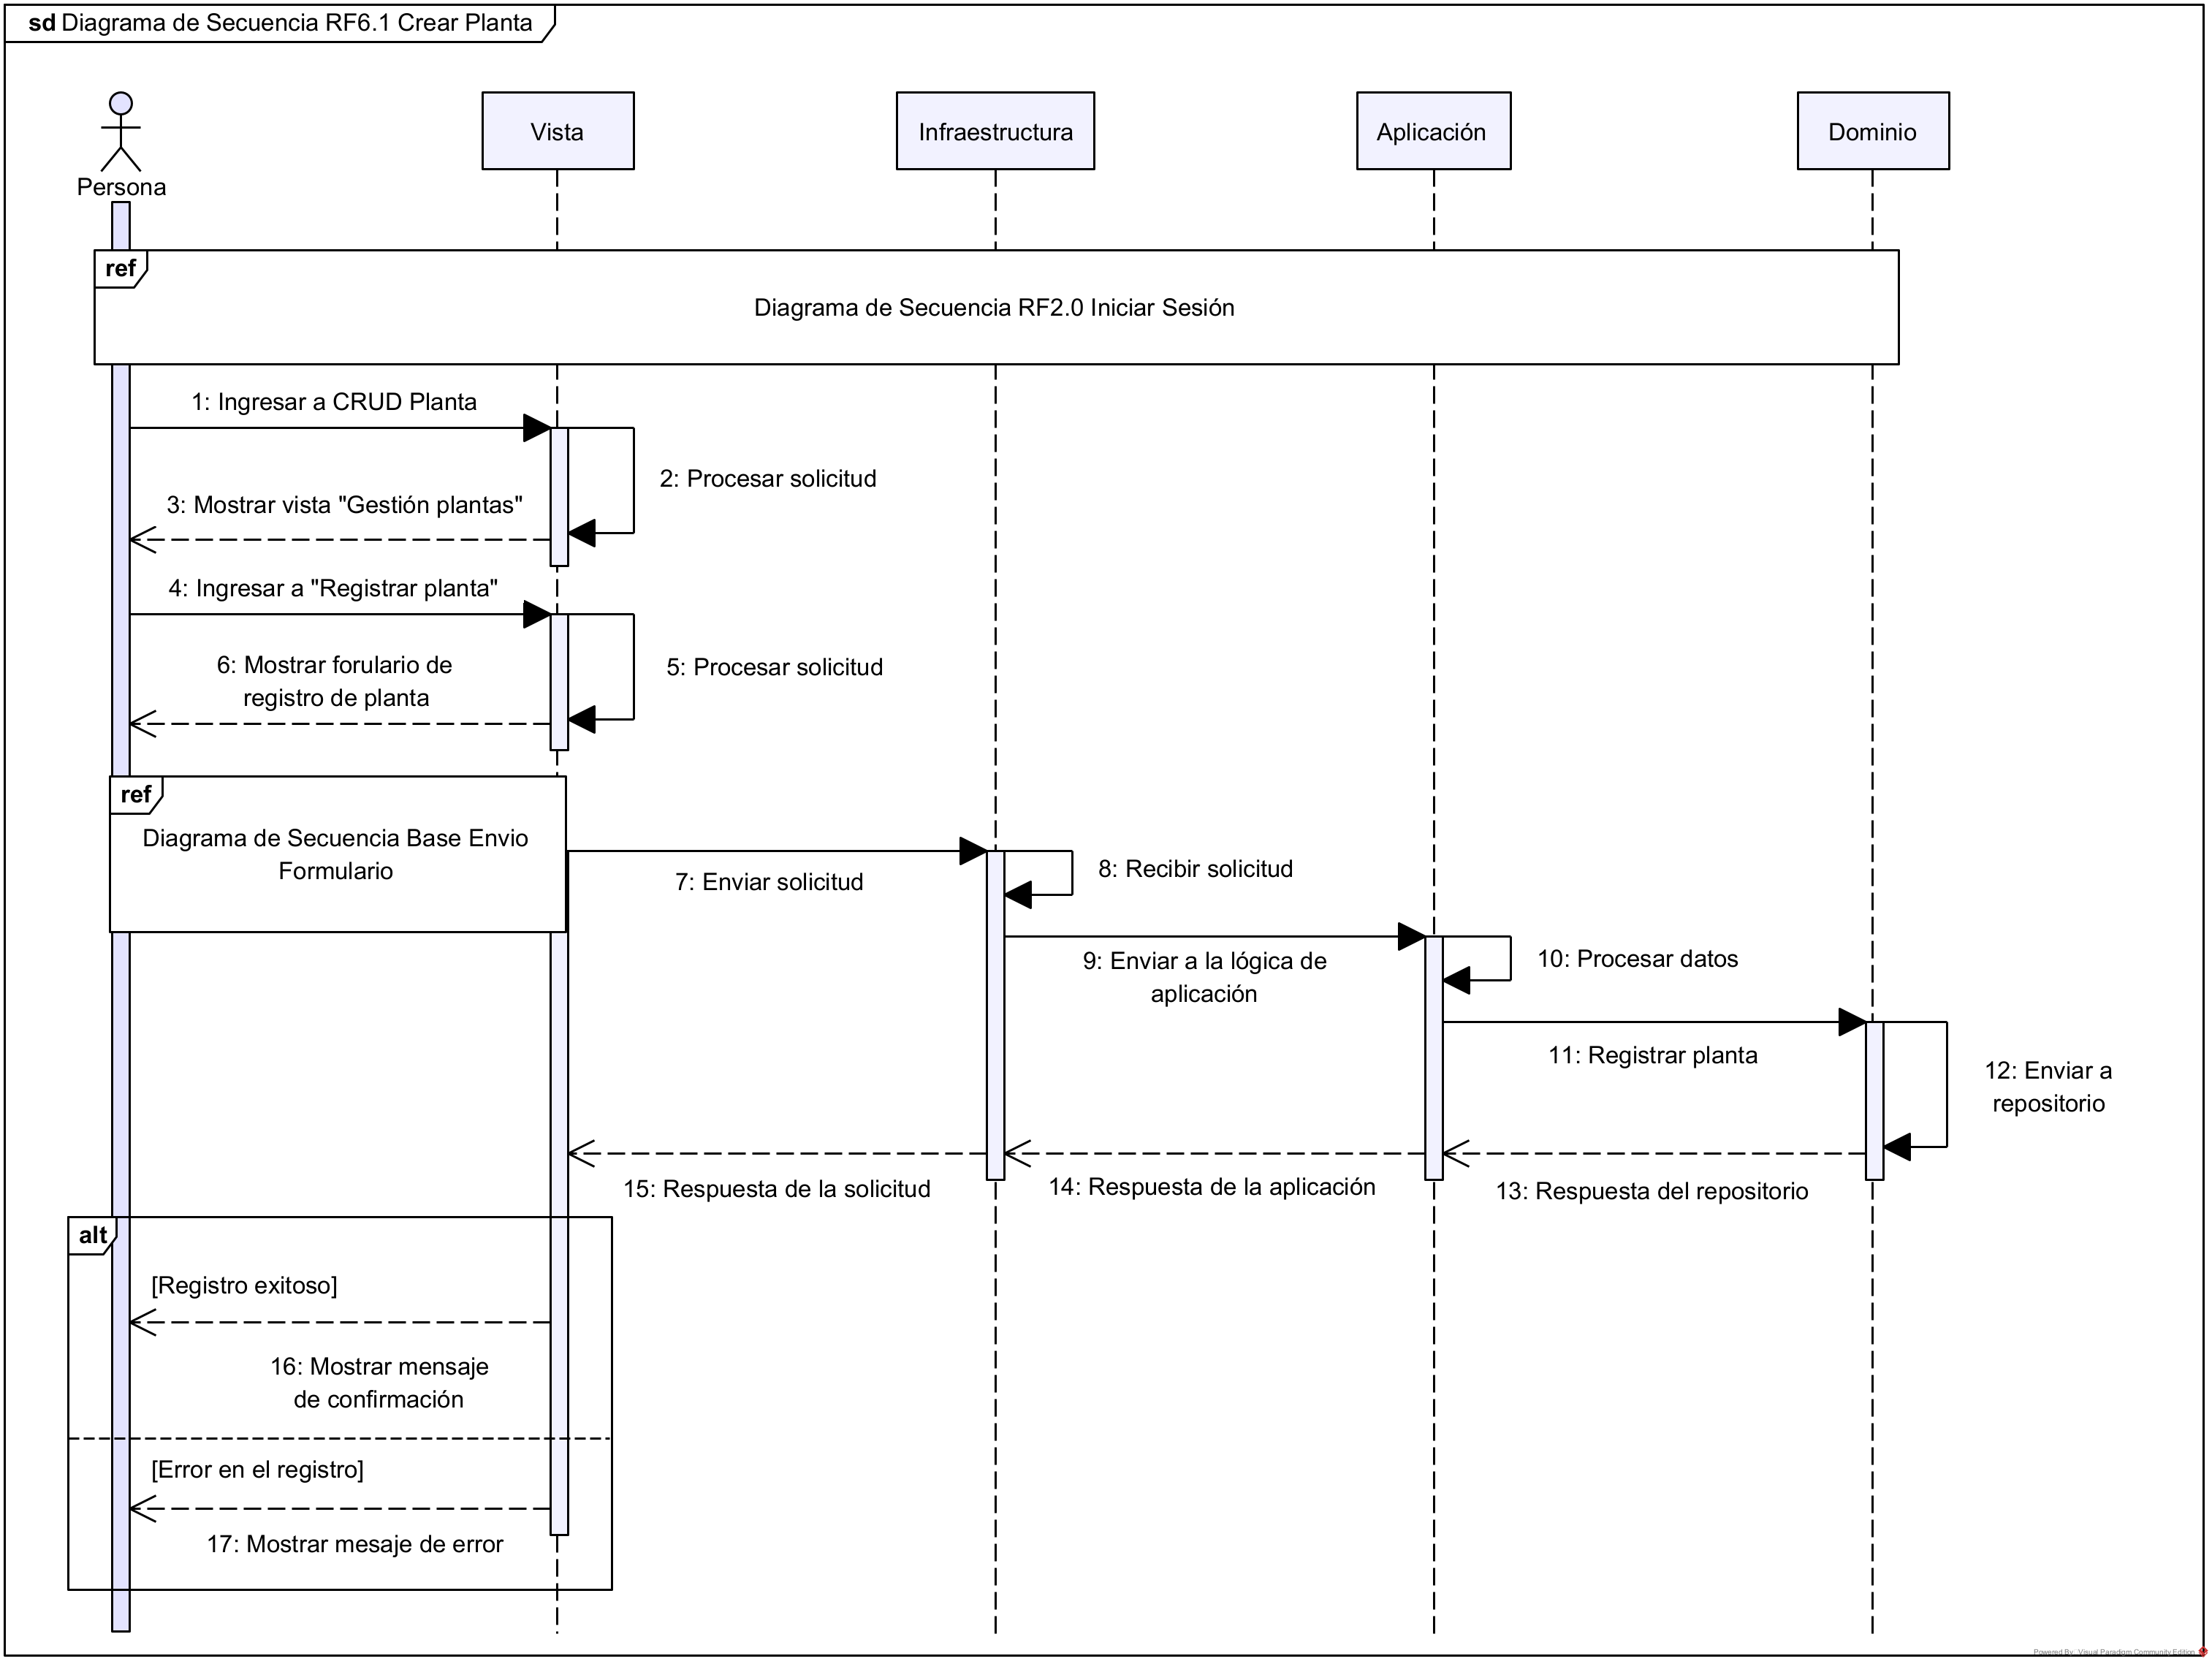
\includegraphics[width=0.8\textwidth]{UML/Secuencia/Diagrama de Secuencia RF6.1 Crear Planta.png}
\end{figure}


\begin{figure}[H]
	\centering
		\caption{Diagrama de Secuencia para Consultar Planta (RF6.2).}
	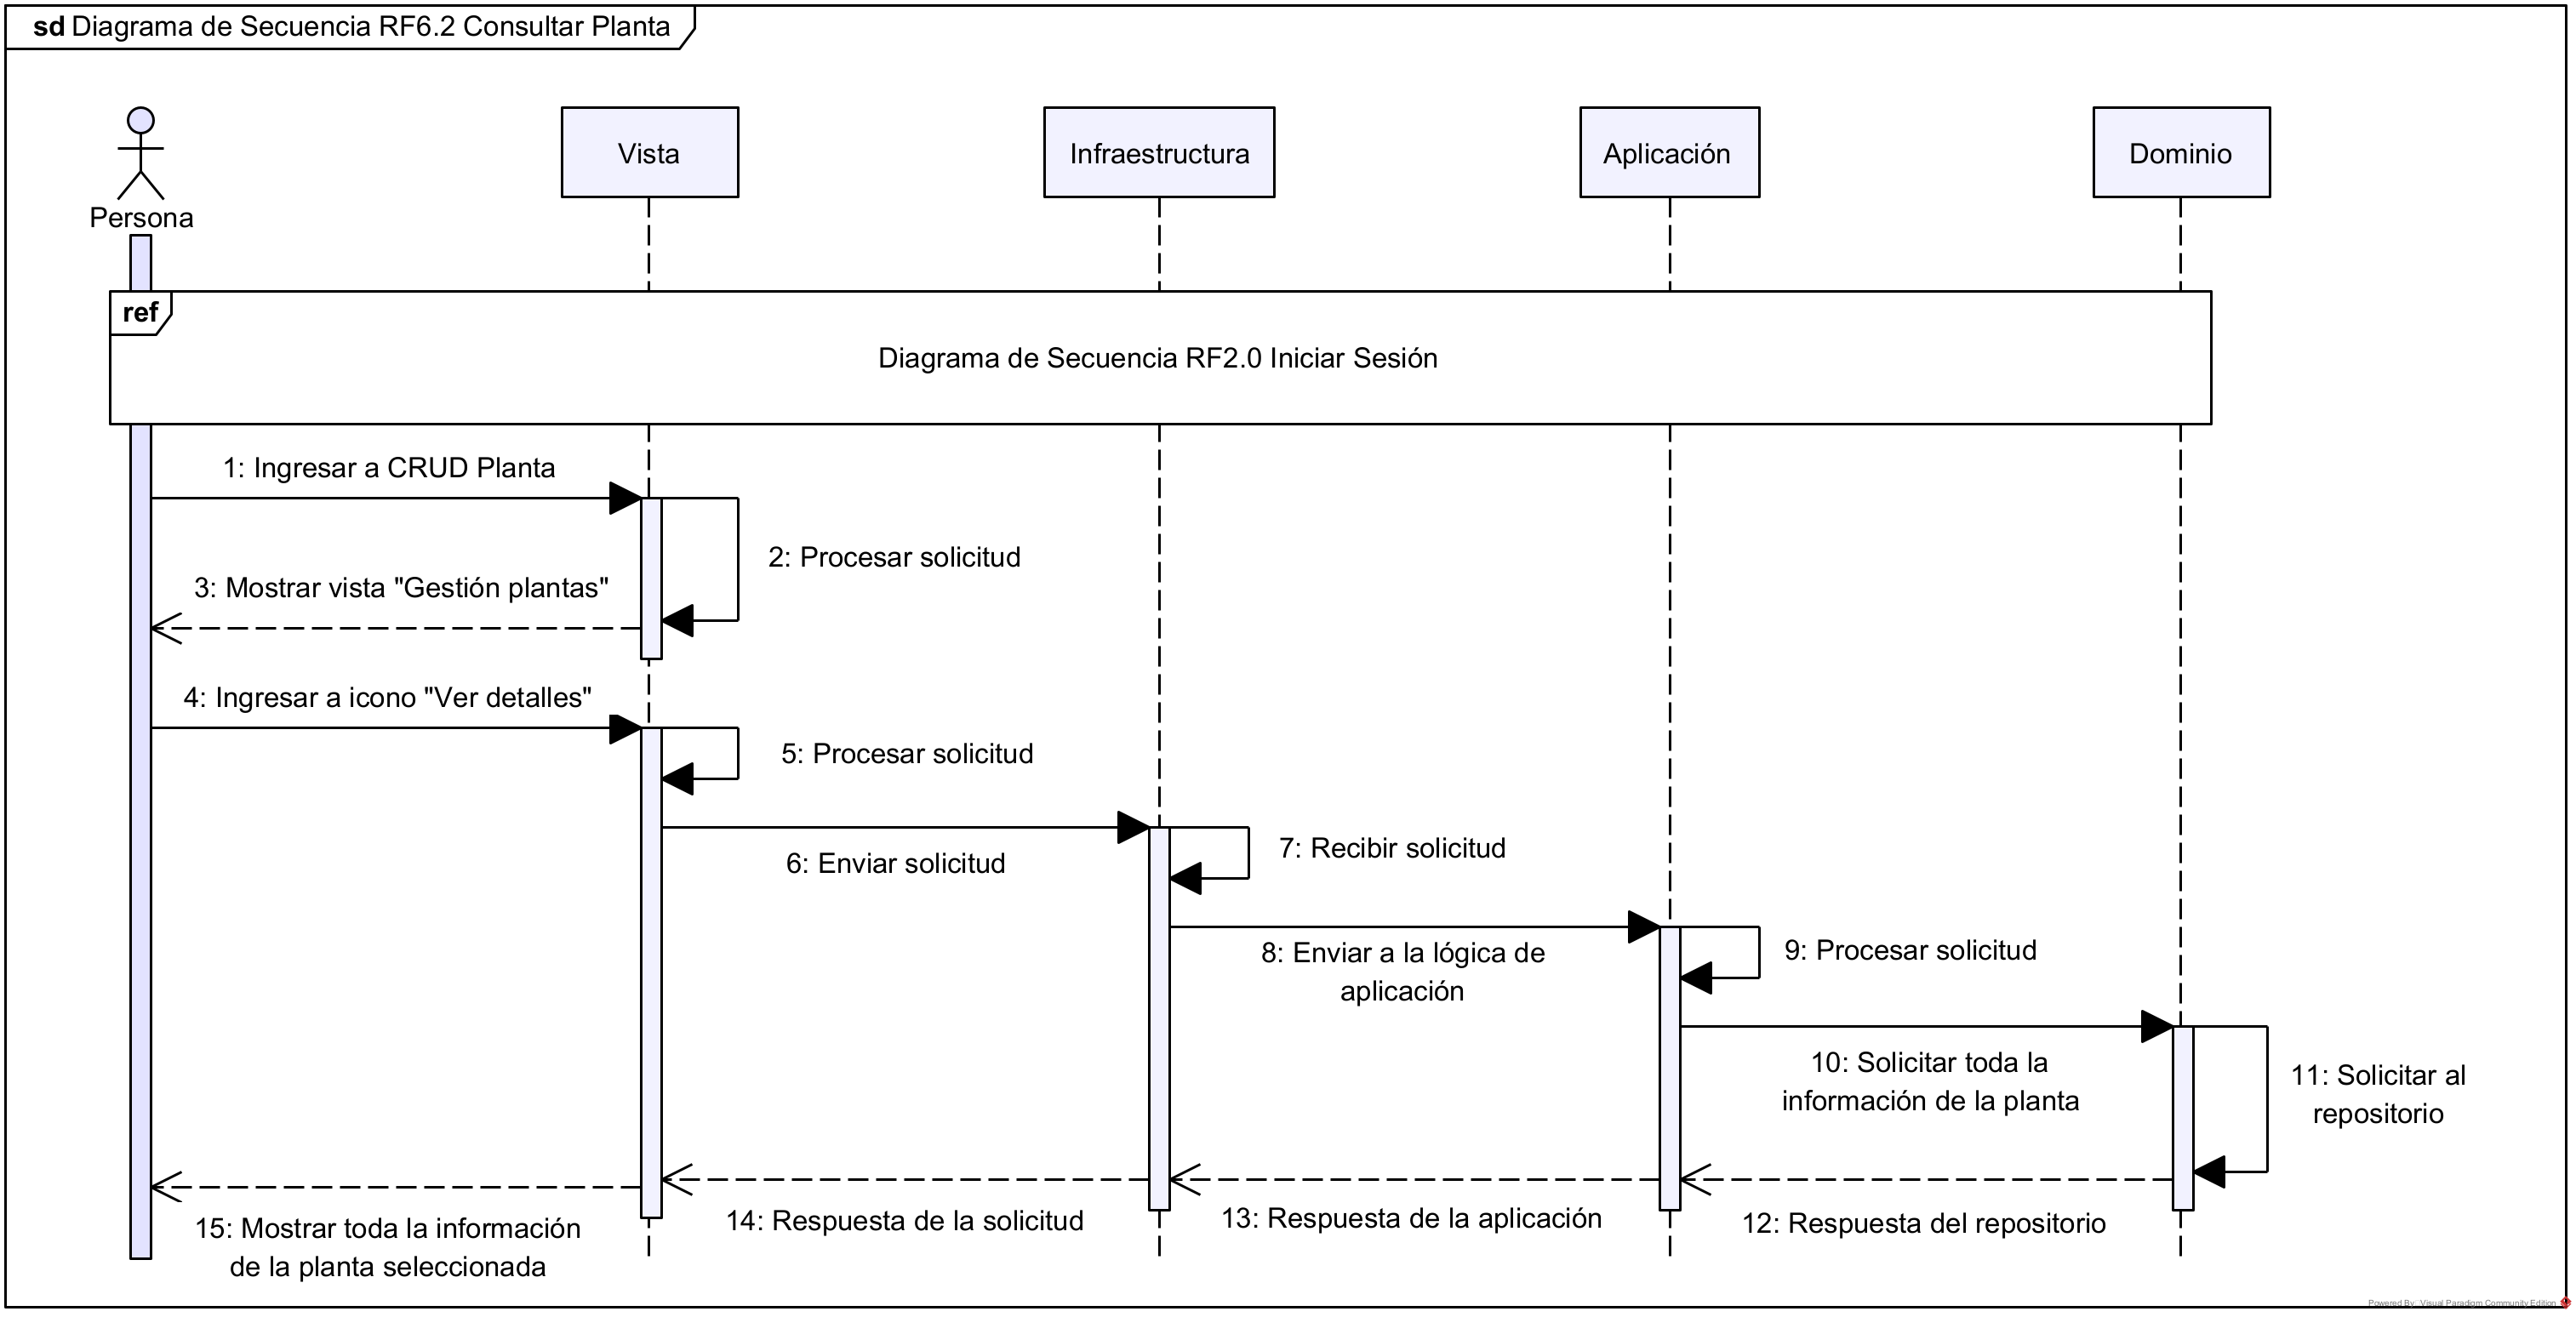
\includegraphics[width=0.8\textwidth]{UML/Secuencia/Diagrama de Secuencia RF6.2 Consultar Planta.png}
\end{figure}


\begin{figure}[H]
	\centering
	\caption{Diagrama de Secuencia para Editar Planta (RF6.3).}
 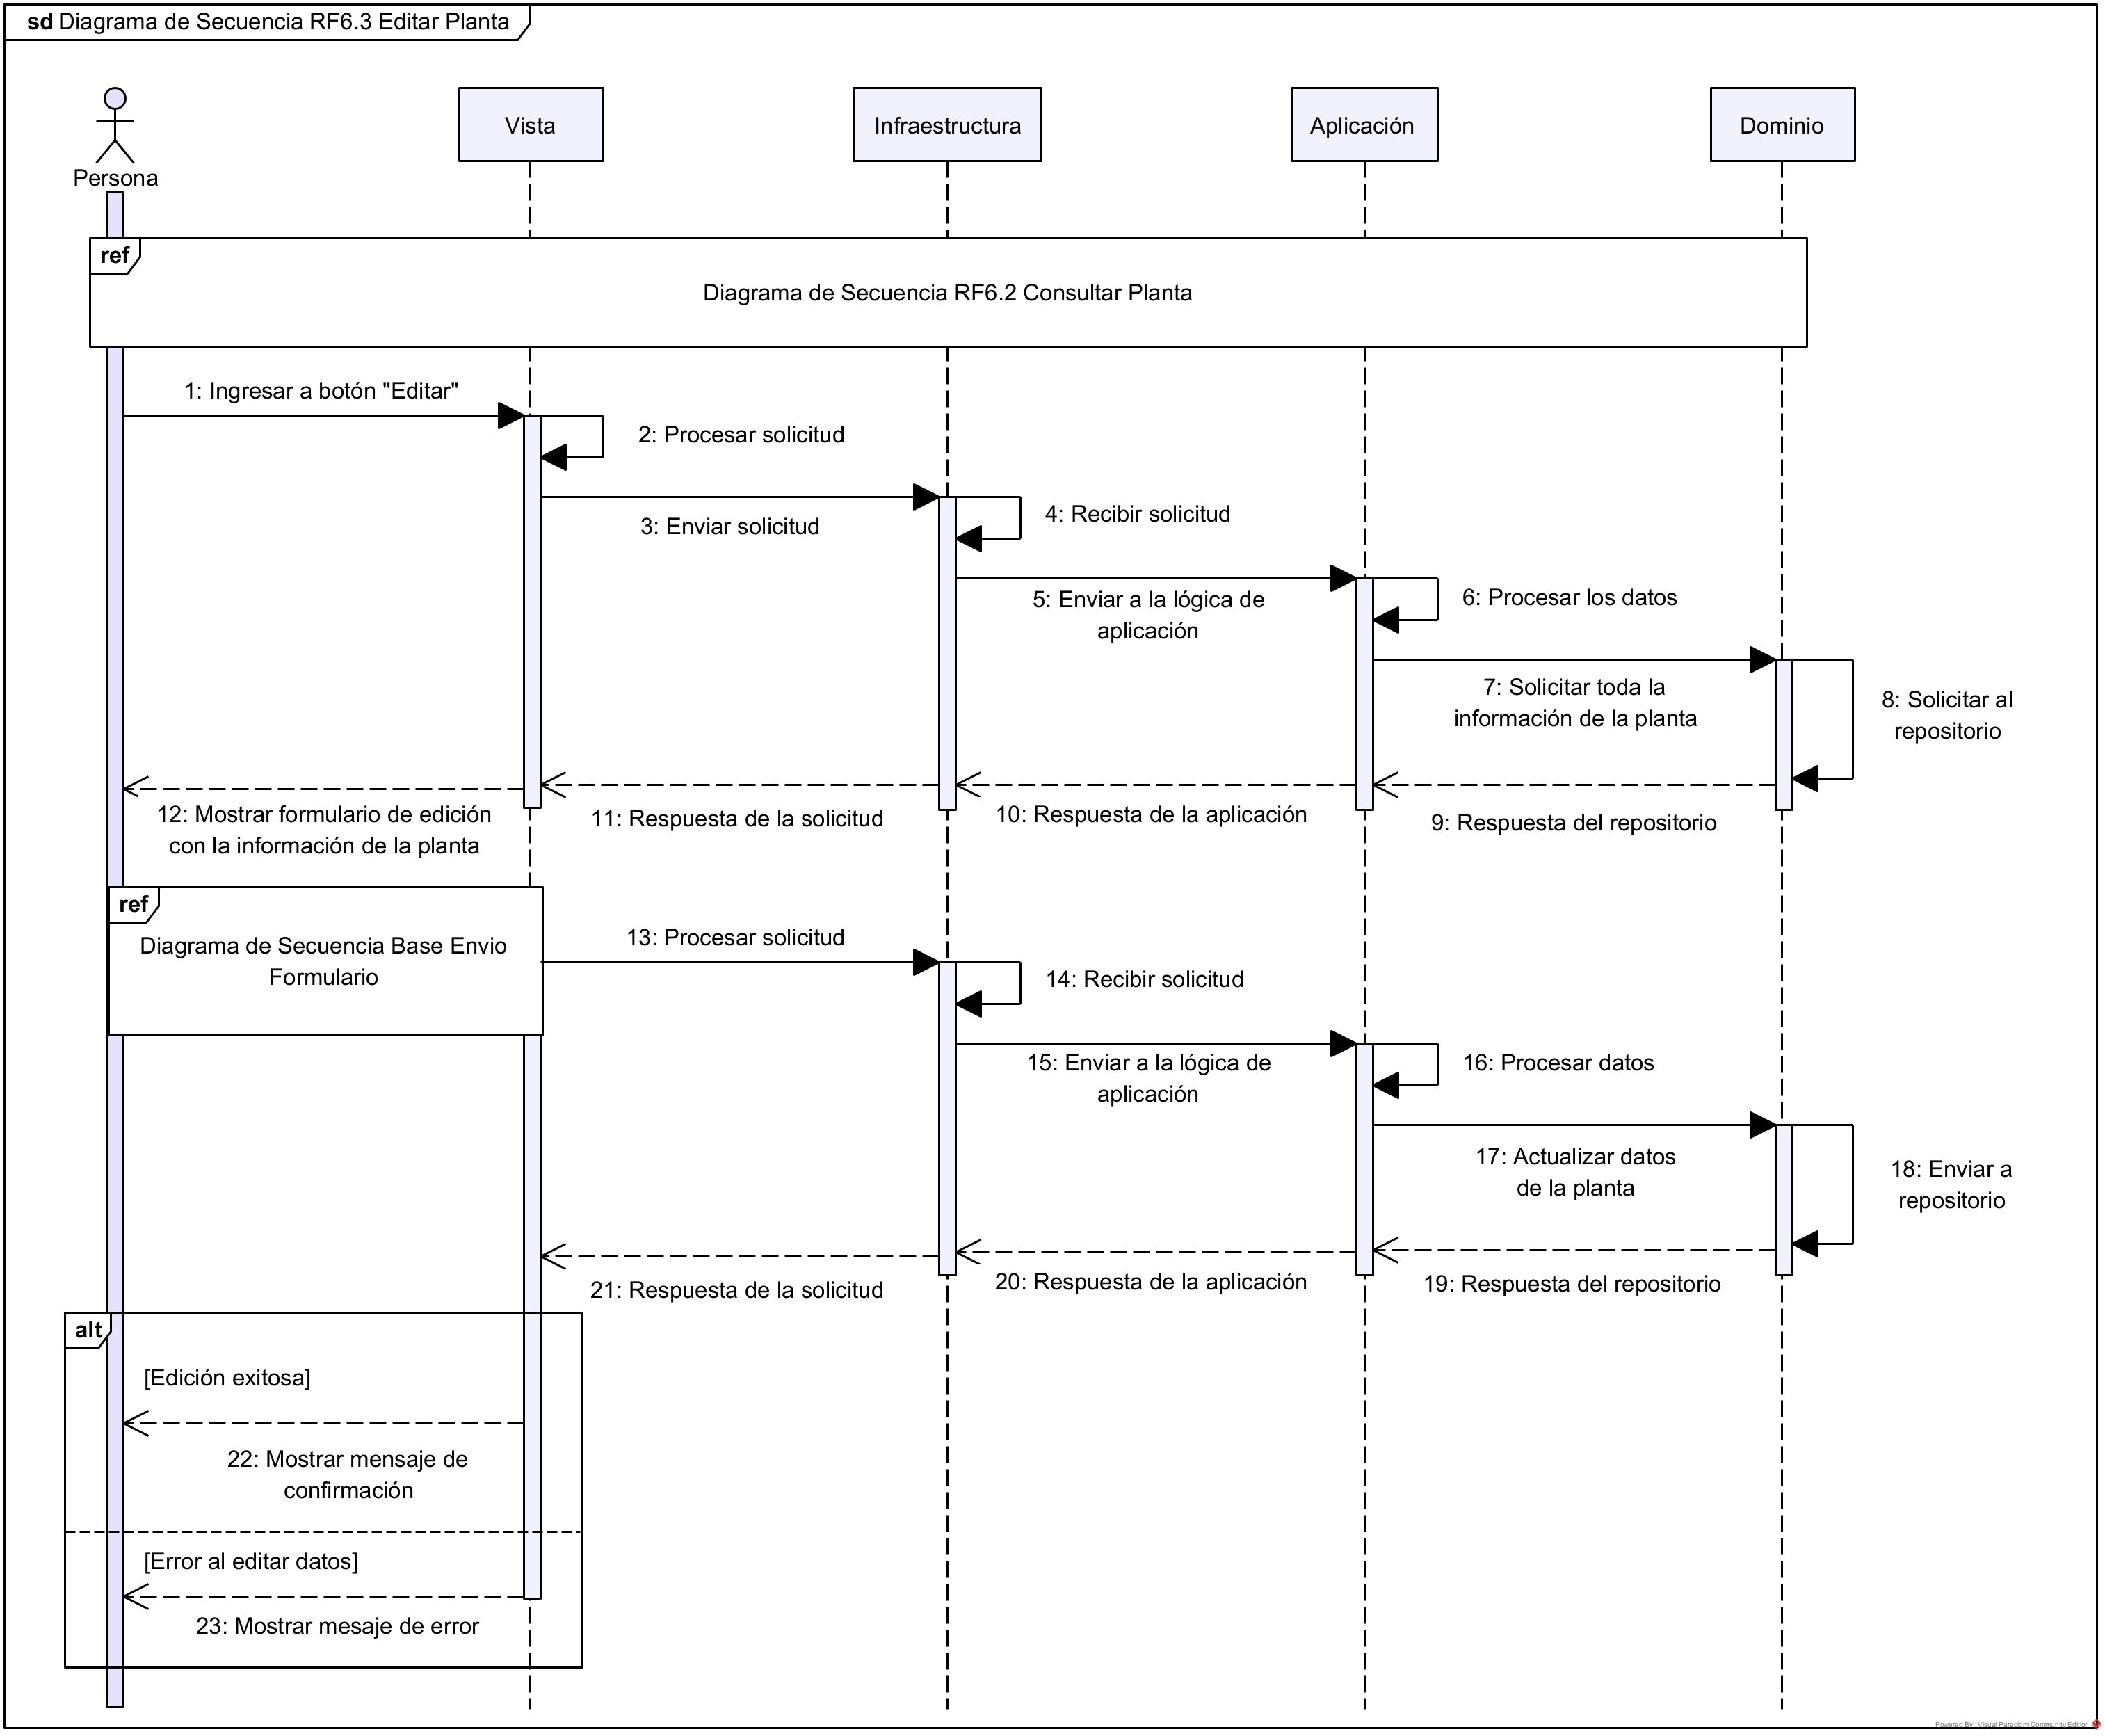
\includegraphics[width=0.8\textwidth]{UML/Secuencia/Diagrama de Secuencia RF6.3 Editar Planta.png}
\end{figure}


\begin{figure}[H]
	\centering
	\caption{Diagrama de Secuencia para Eliminar Planta (RF6.4).}
 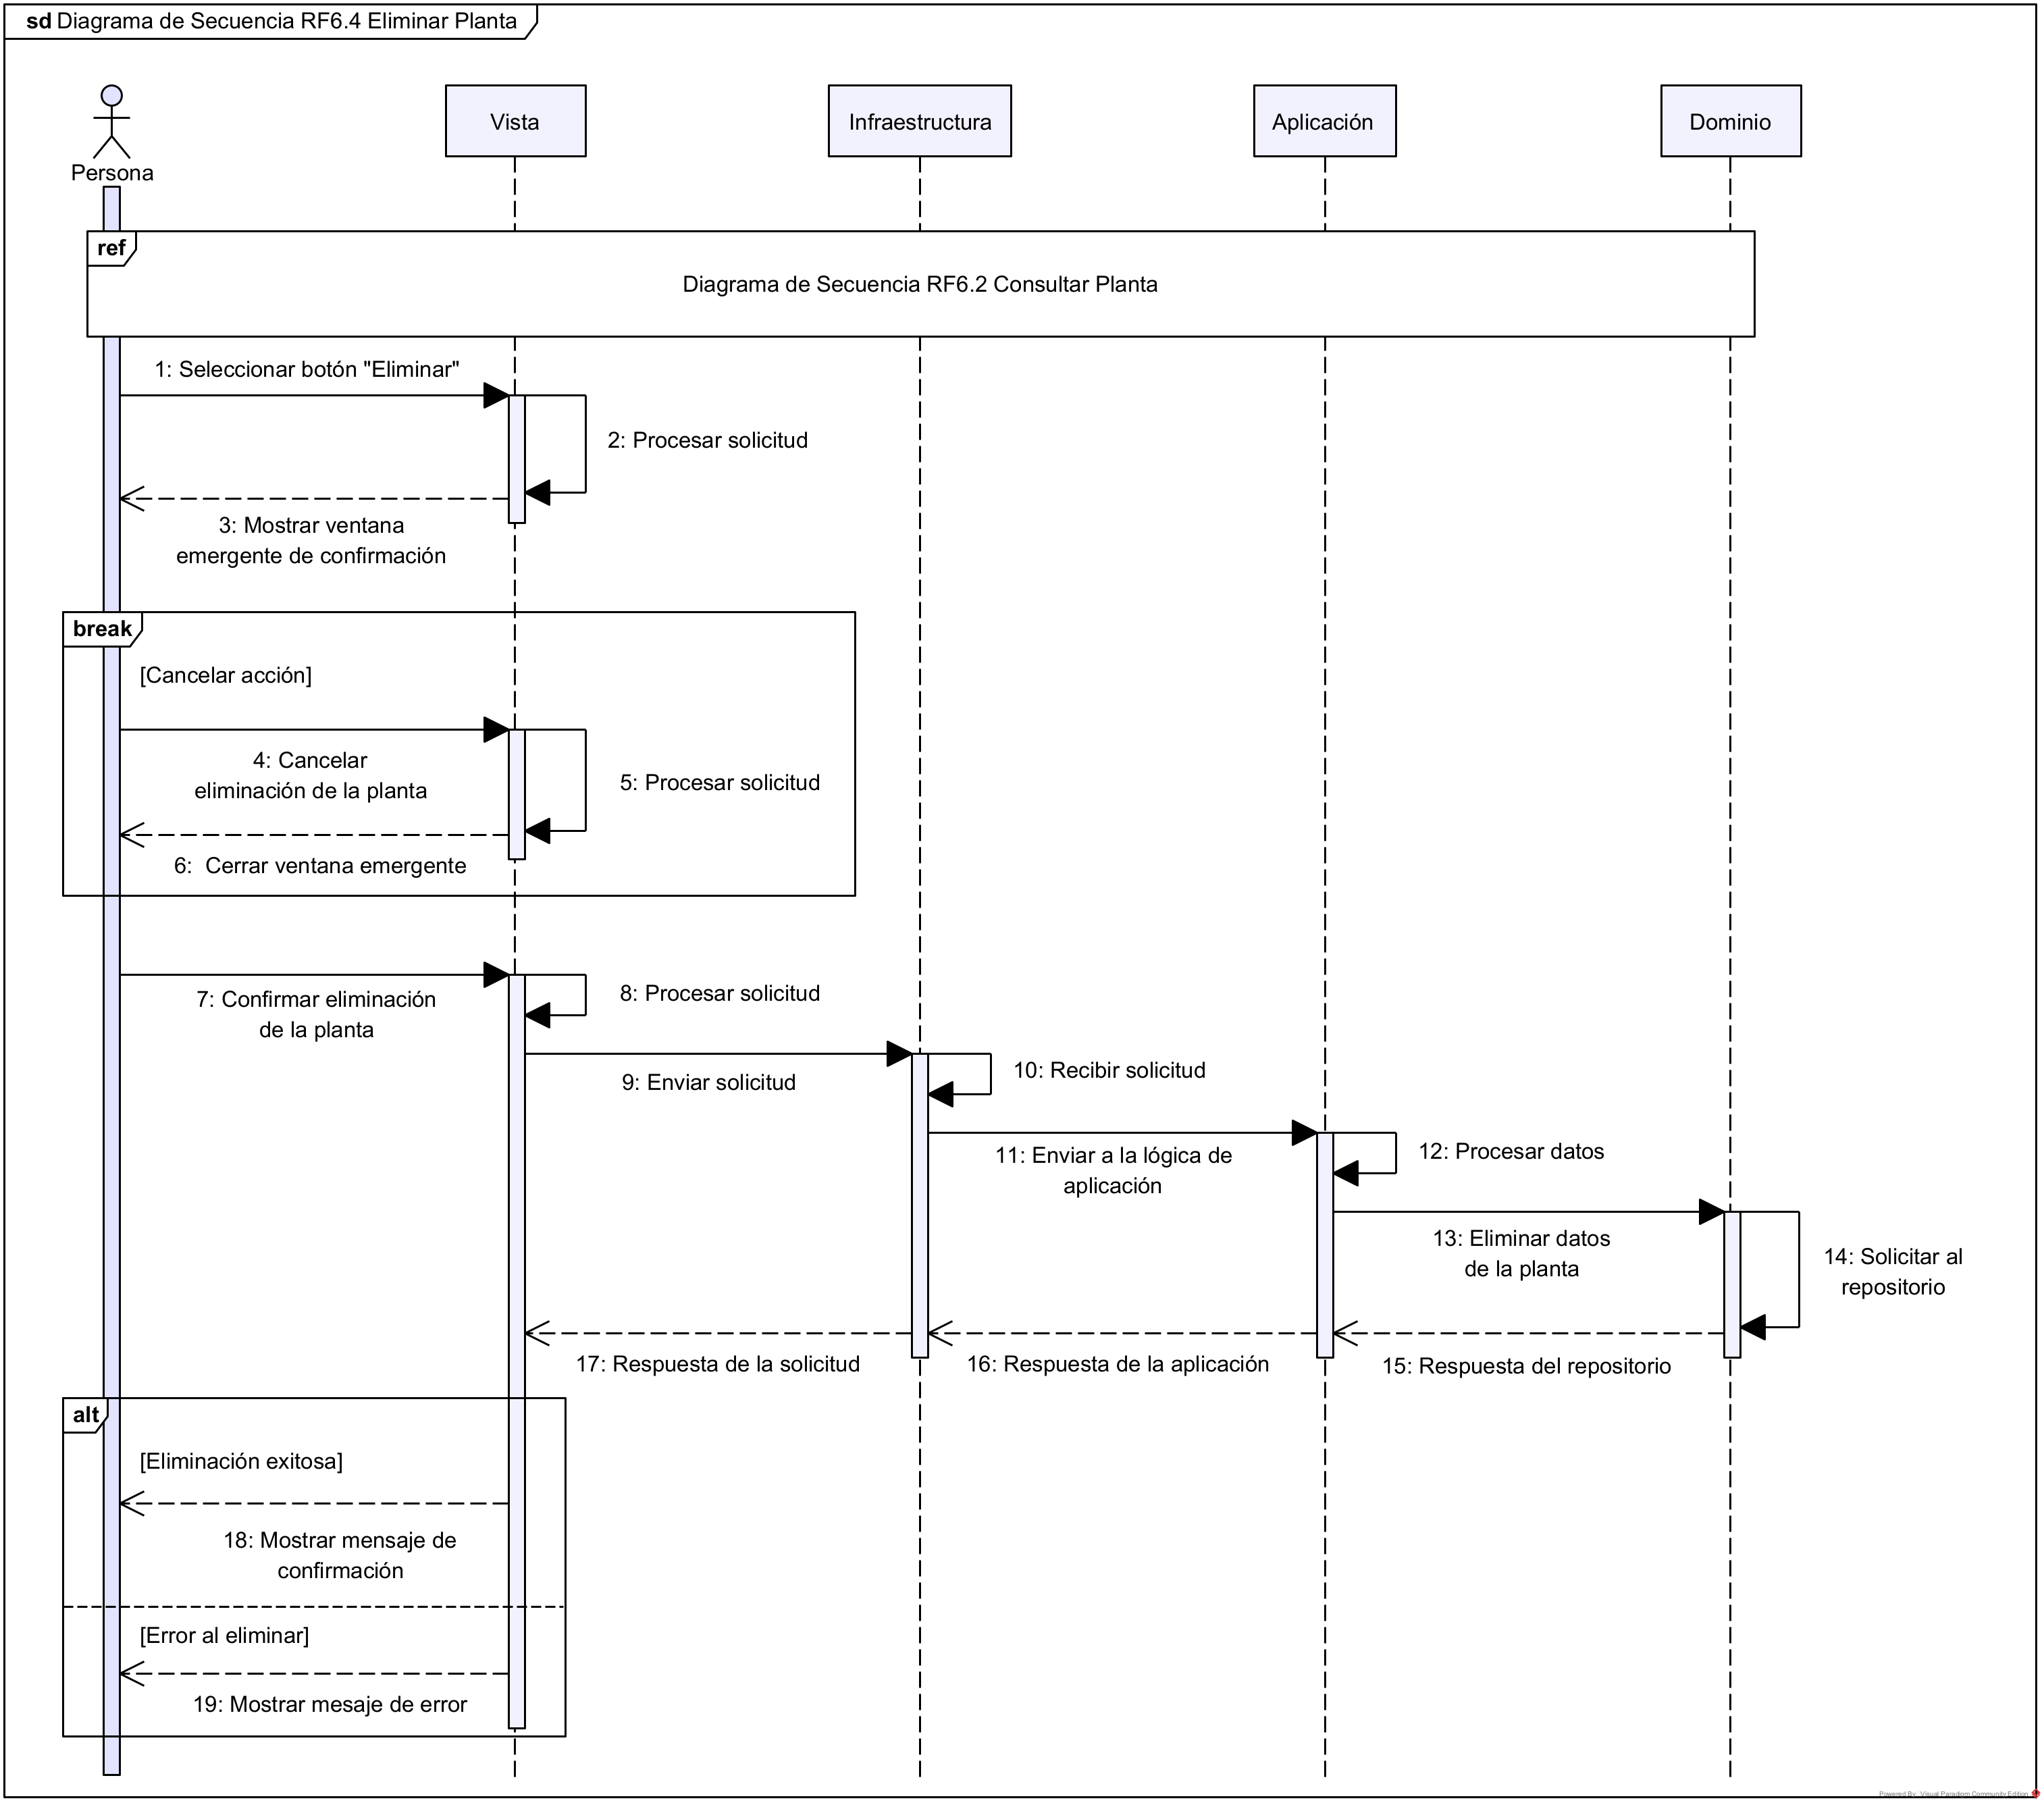
\includegraphics[width=0.8\textwidth]{UML/Secuencia/Diagrama de Secuencia RF6.4 Eliminar Planta.png}
\end{figure}


\begin{figure}[H]
	\centering
		\caption{Diagrama de Secuencia para Generar Reporte (RF7.0).}
	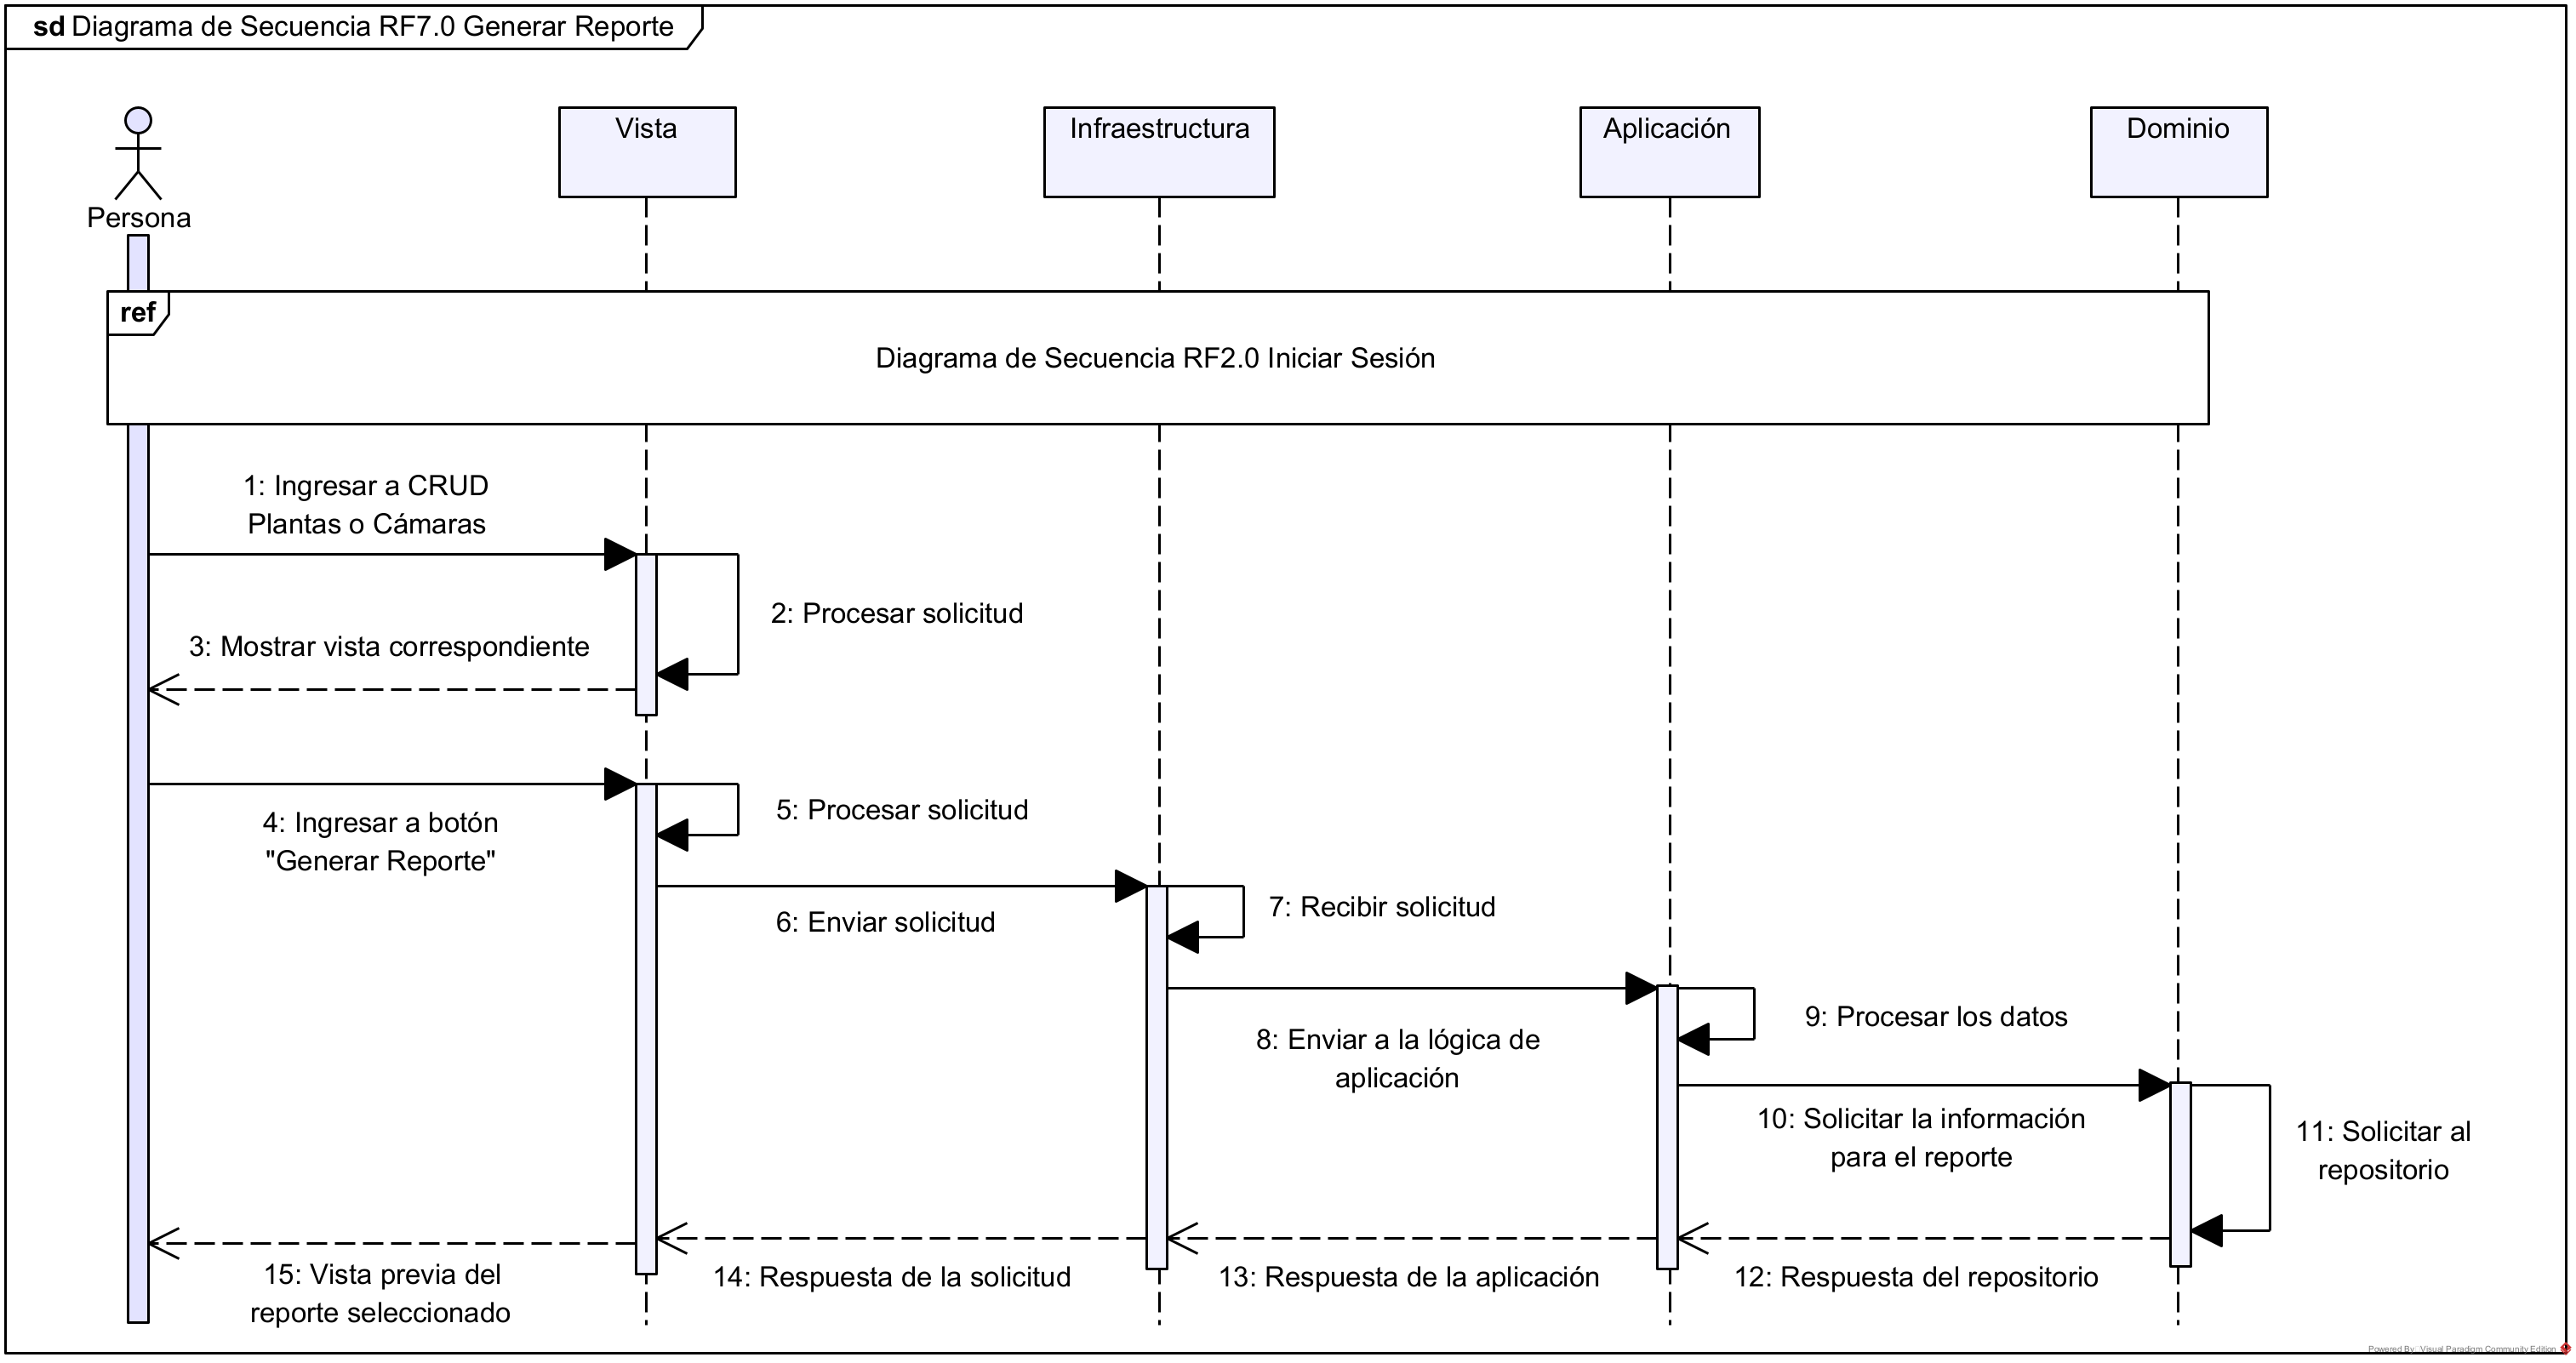
\includegraphics[width=0.8\textwidth]{UML/Secuencia/Diagrama de Secuencia RF7.0 Generar Reporte.png}
\end{figure}


\begin{figure}[H]
	\centering
	\caption{Diagrama de Secuencia para Descargar Reporte (RF7.1).}
 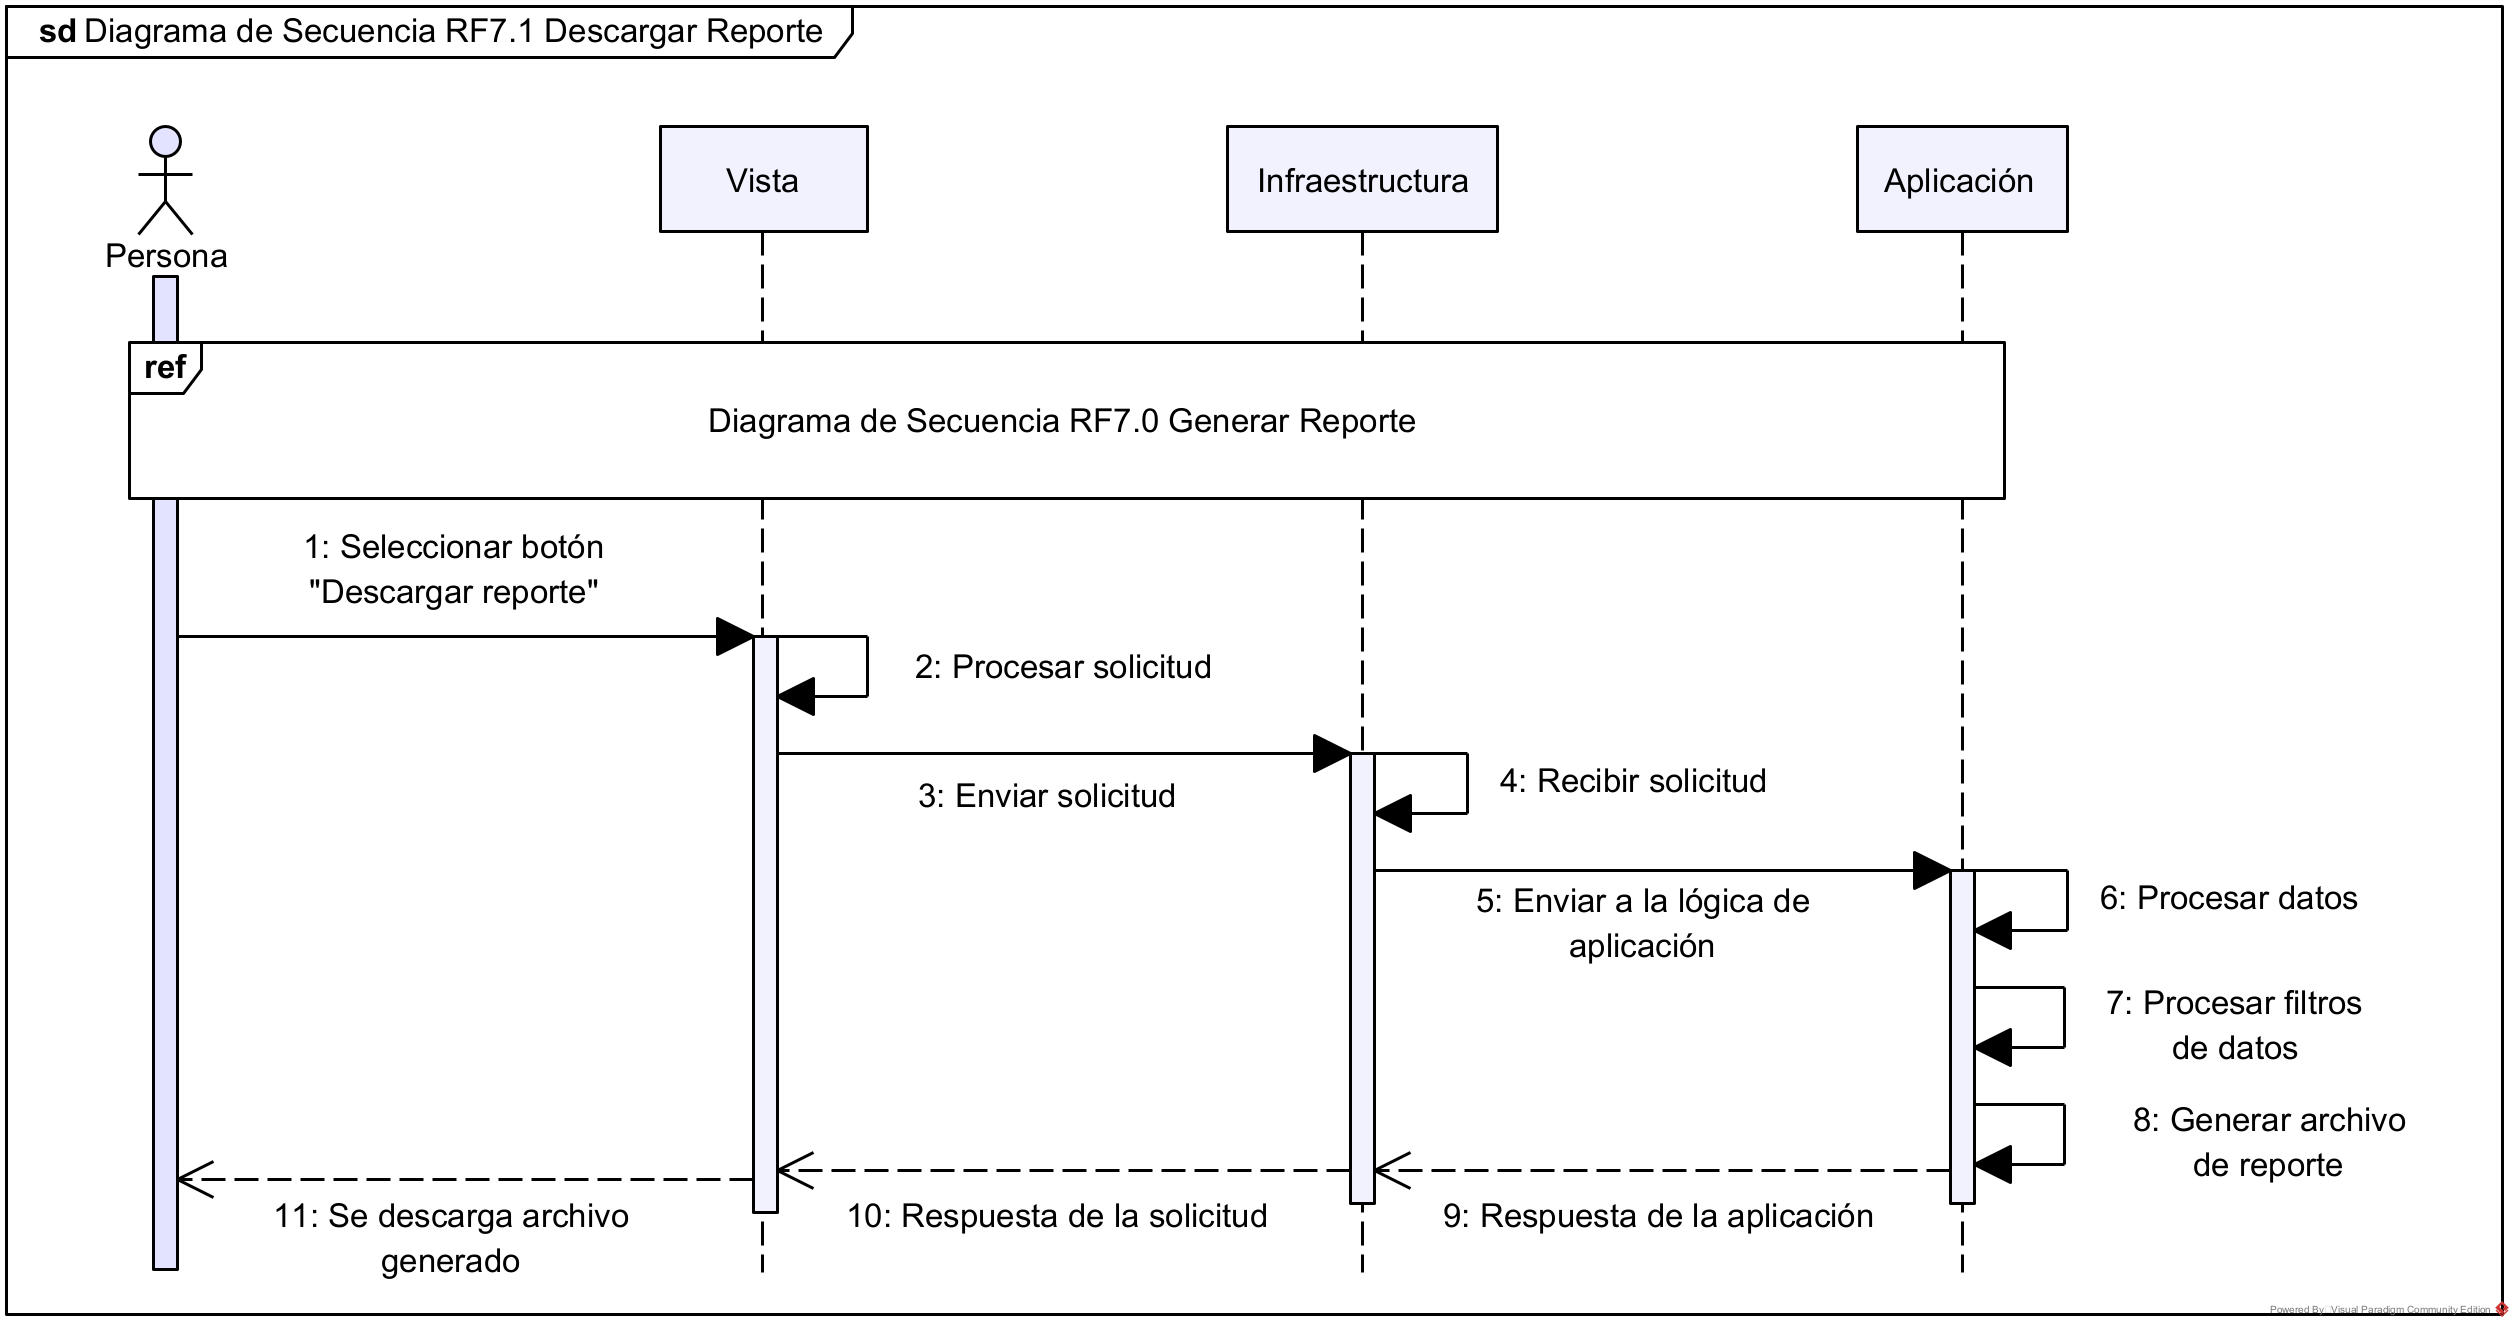
\includegraphics[width=0.8\textwidth]{UML/Secuencia/Diagrama de Secuencia RF7.1 Descargar Reporte.png}
\end{figure}


\begin{figure}[H]
	\centering
		\caption{Diagrama de Secuencia para Adjuntar Reporte (RF7.2).}
	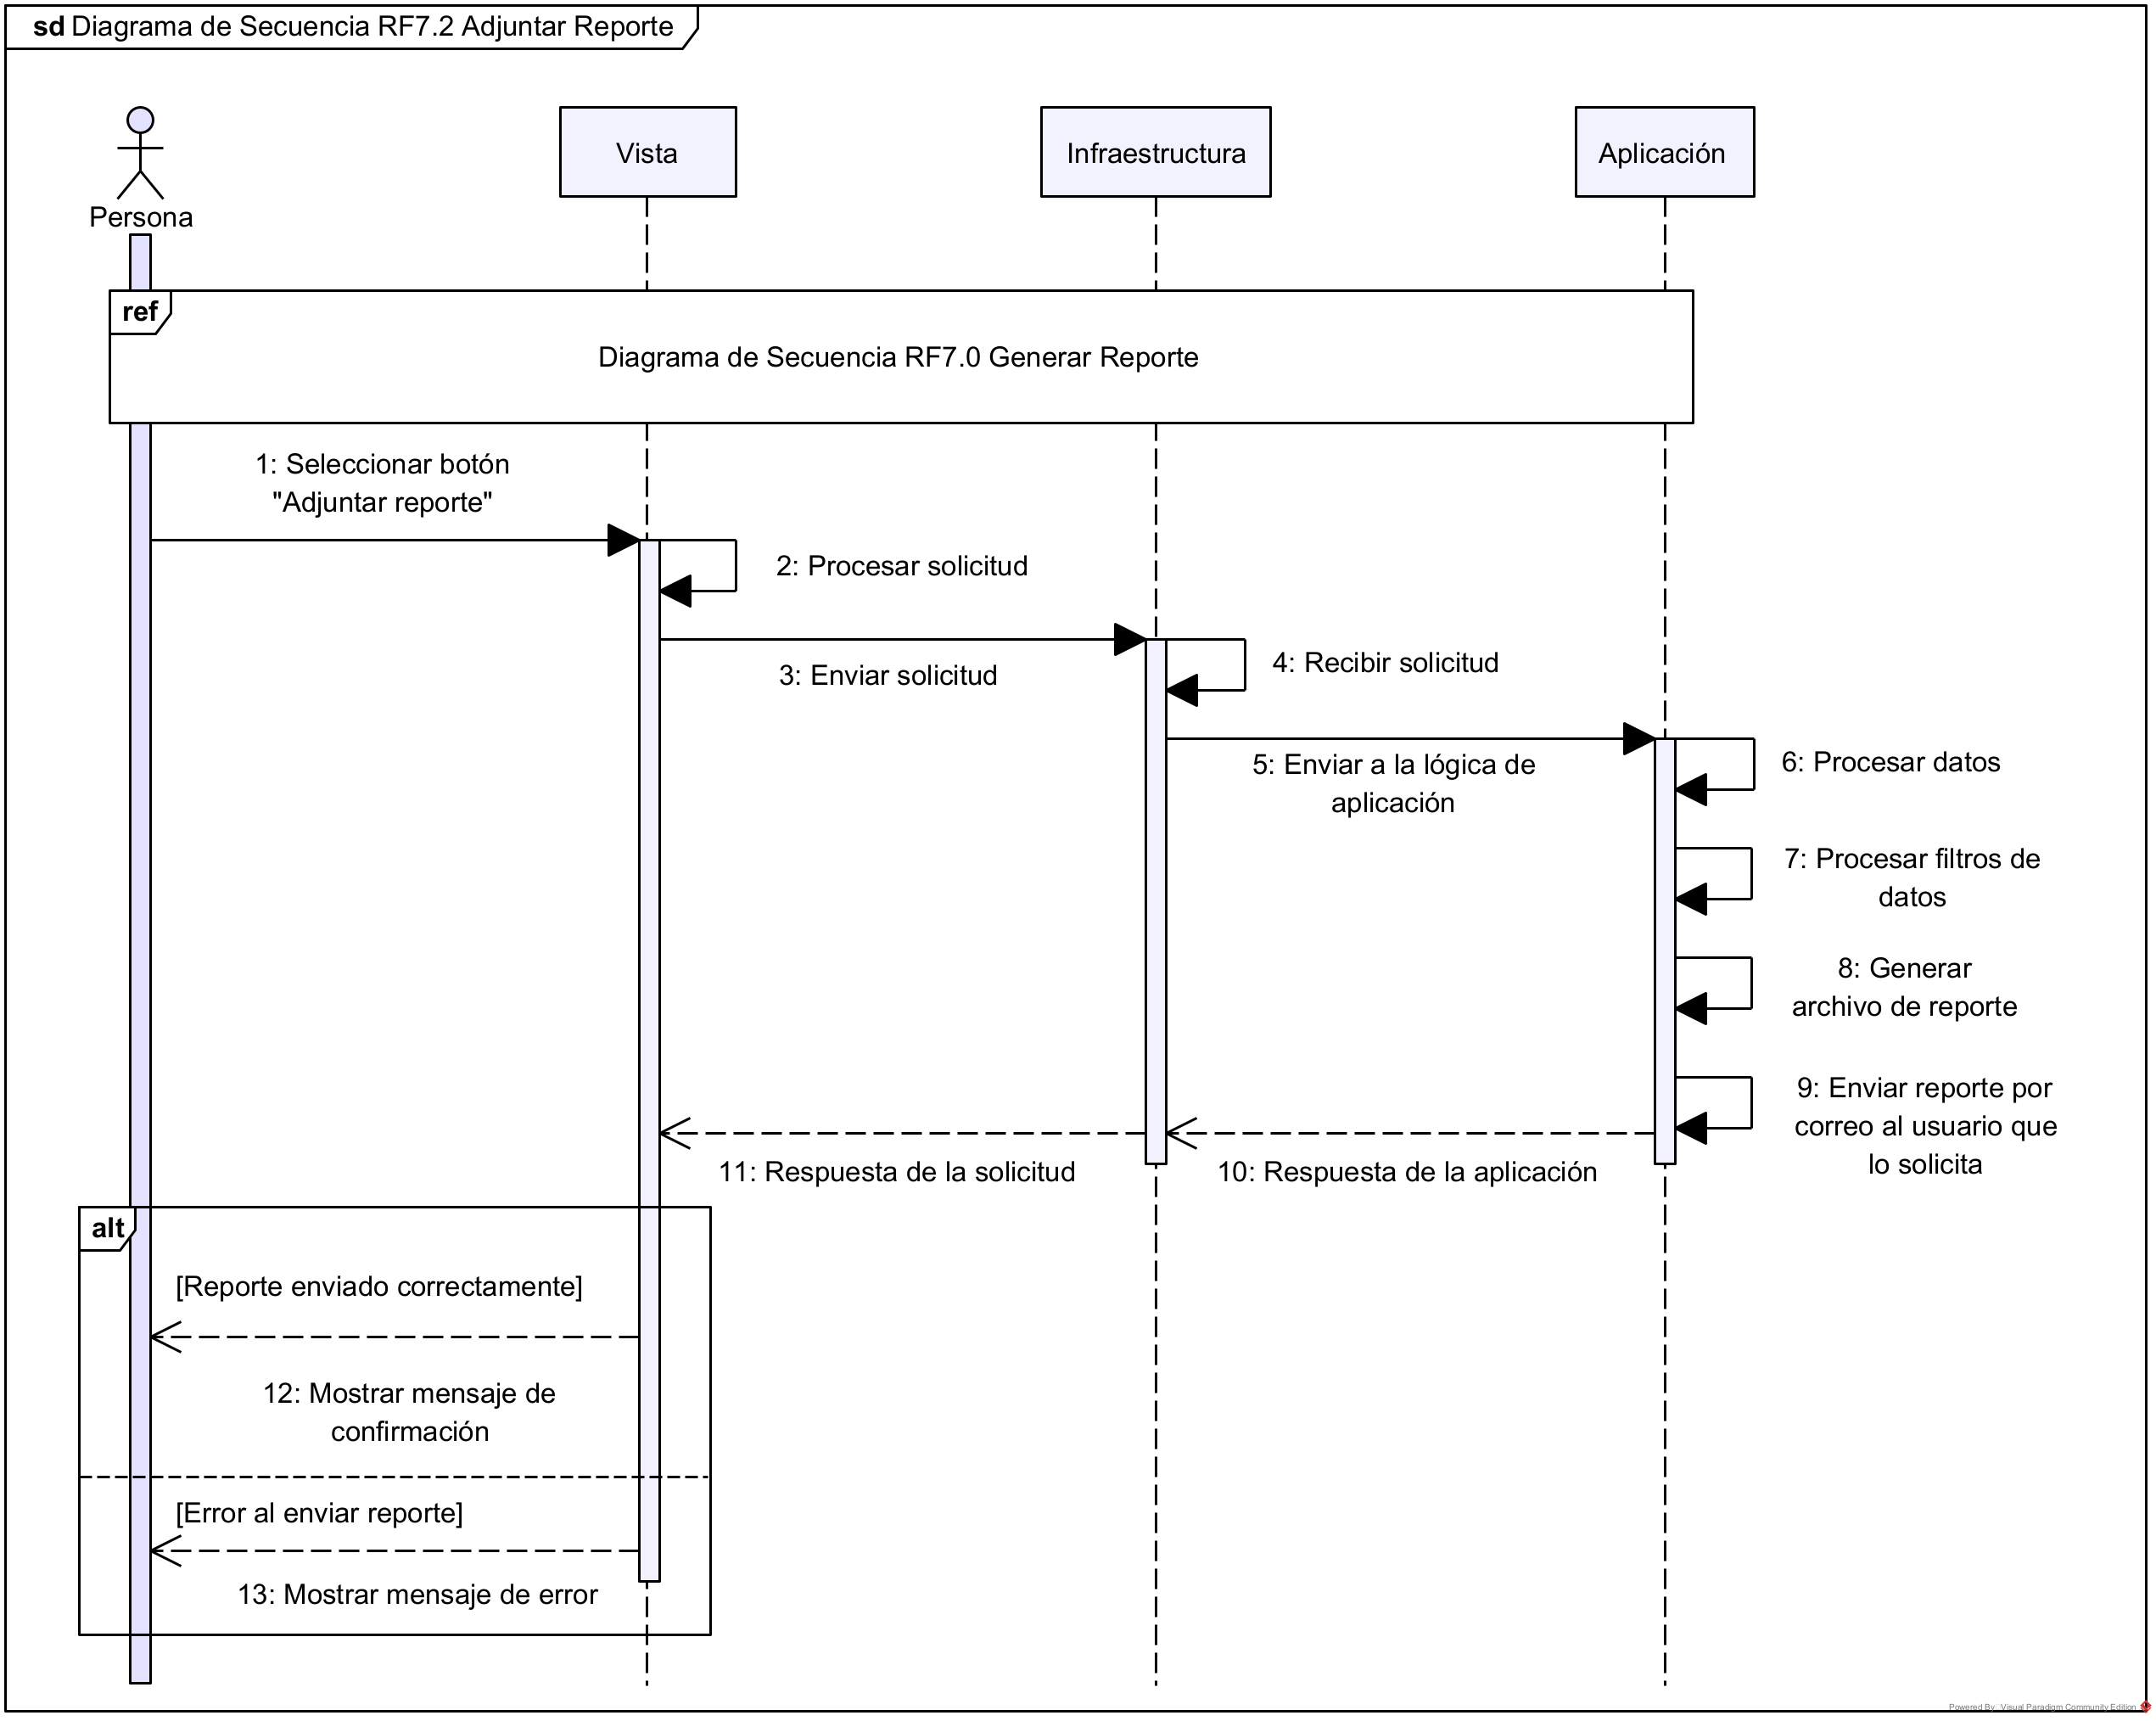
\includegraphics[width=0.8\textwidth]{UML/Secuencia/Diagrama de Secuencia RF7.2 Adjuntar Reporte.png}
\end{figure}


\begin{figure}[H]
	\centering
	\caption{Diagrama de Secuencia para Notificar Planta (RF8.1).}
 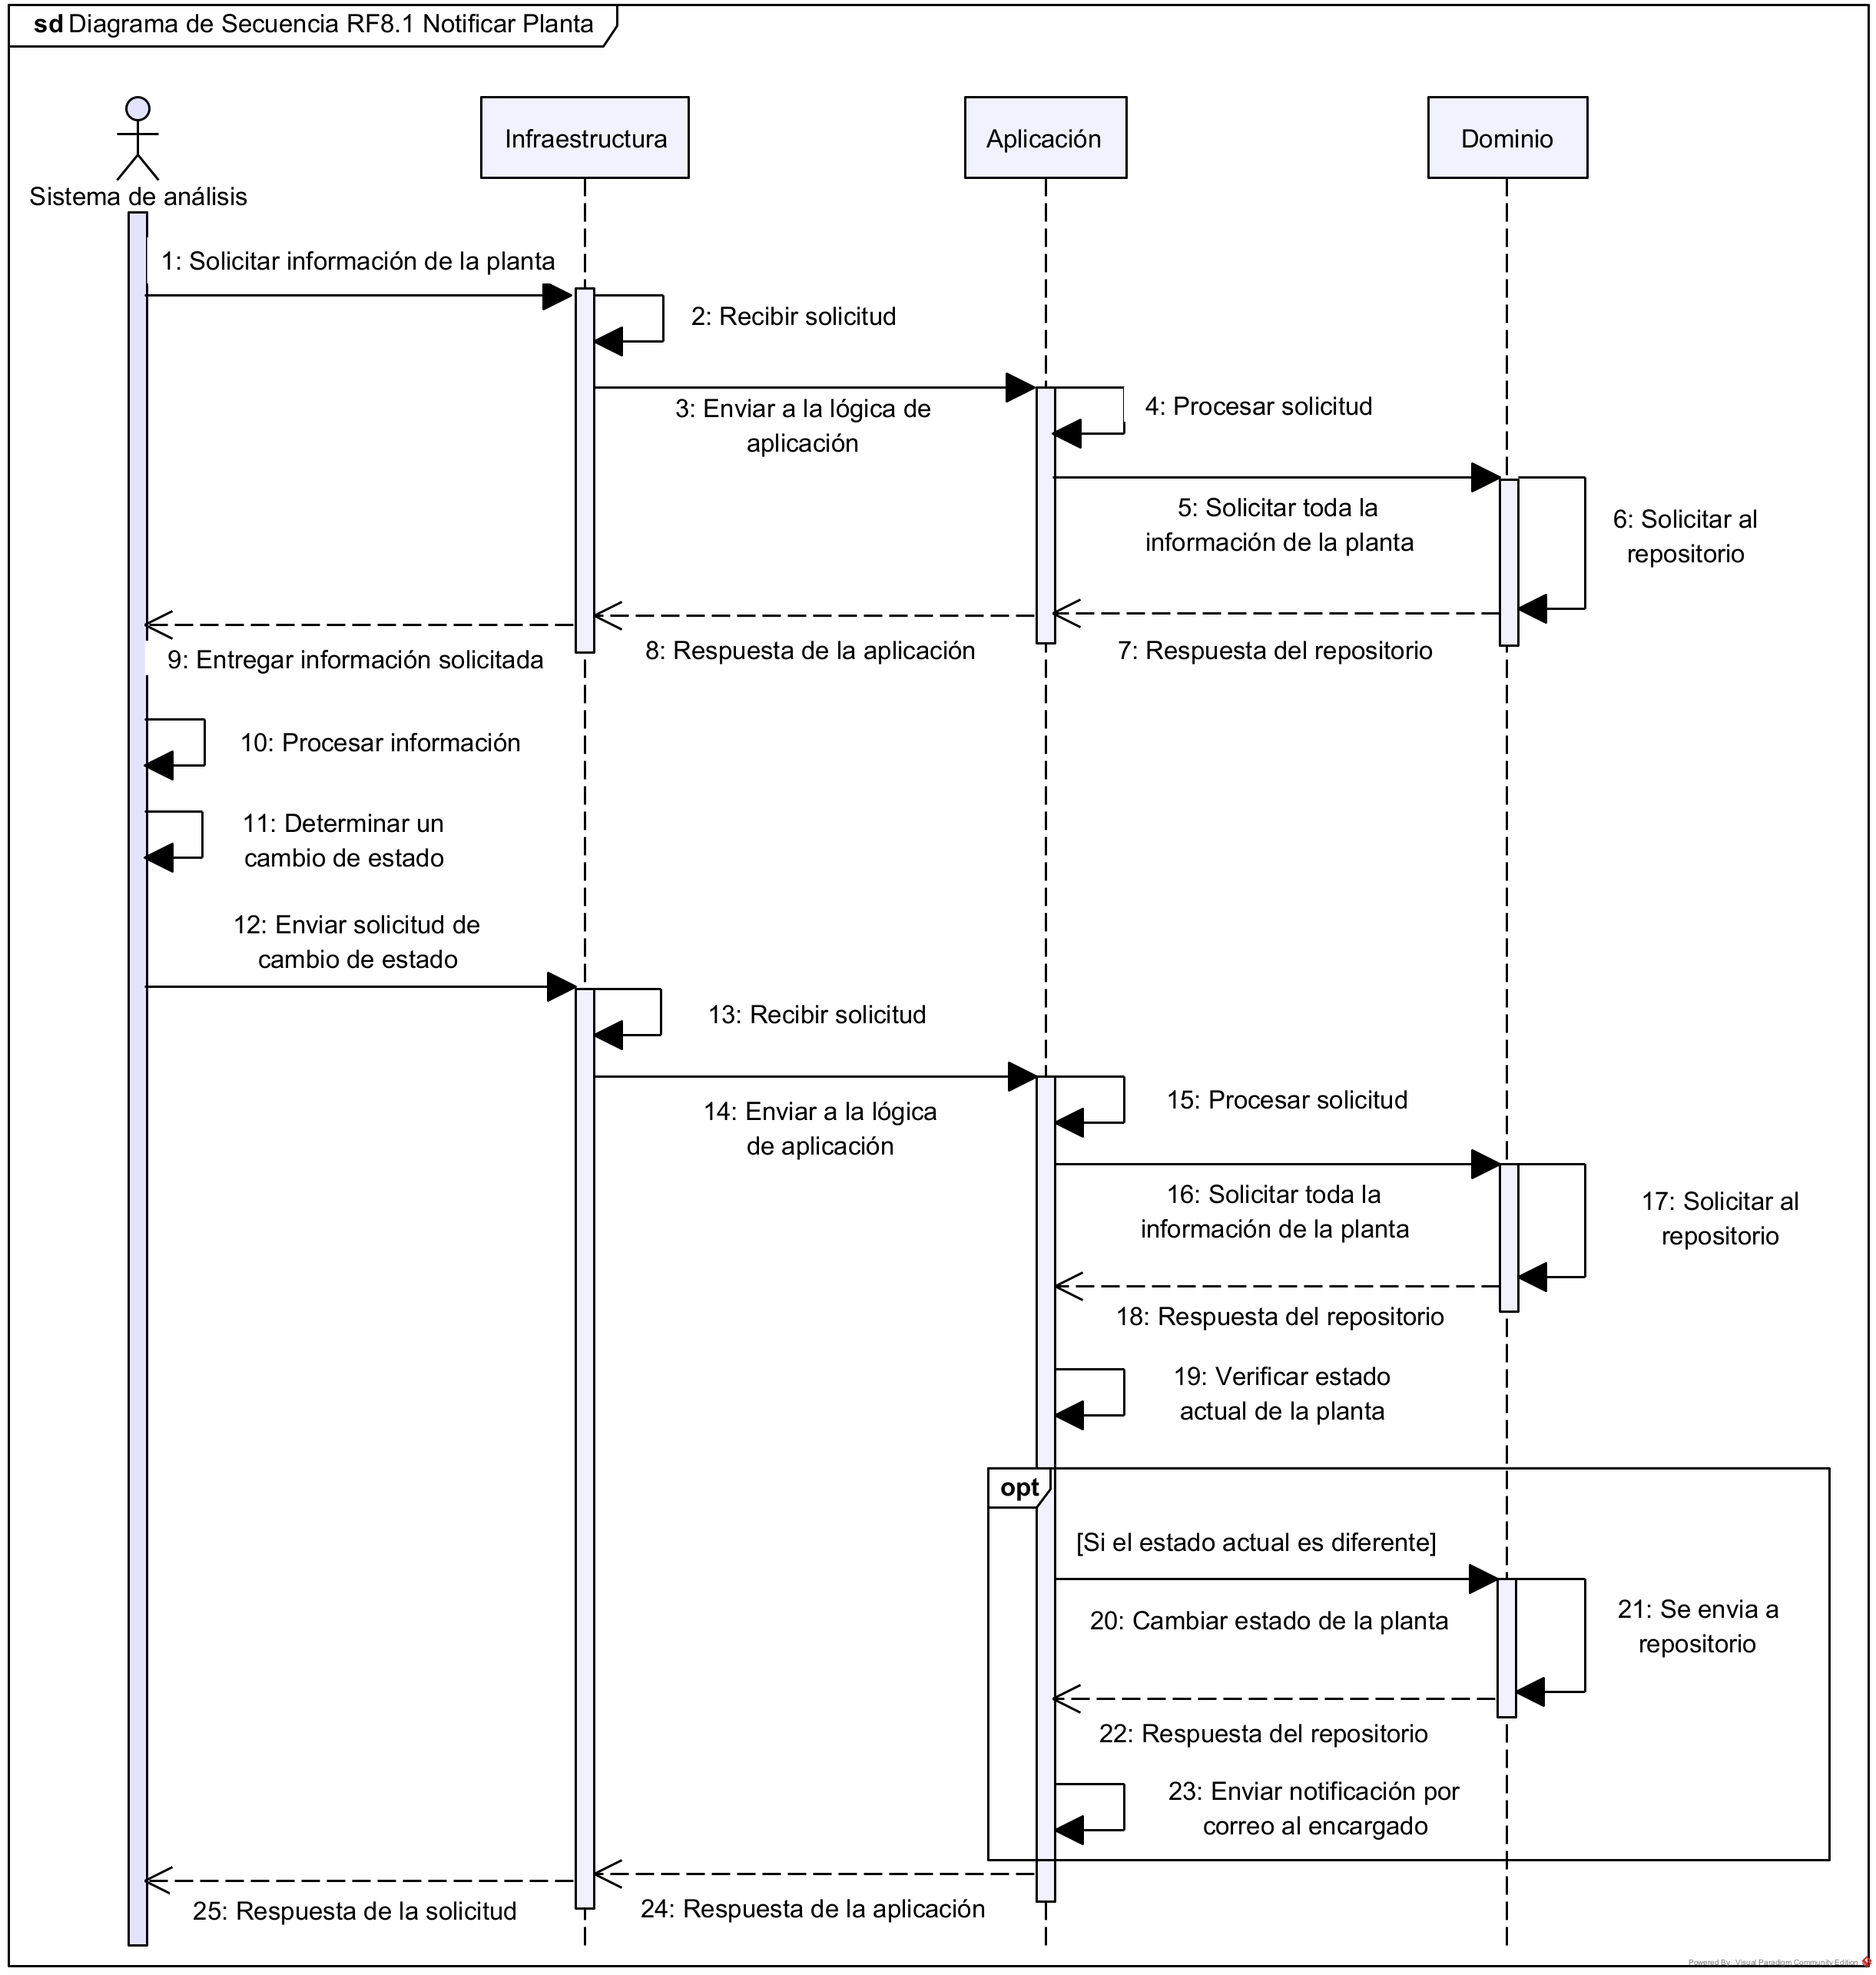
\includegraphics[width=0.8\textwidth]{UML/Secuencia/Diagrama de Secuencia RF8.1 Notificar Planta.png}
\end{figure}


\begin{figure}[H]
	\centering
	\caption{Diagrama de Secuencia para Notificar Seguridad (RF8.2).}
 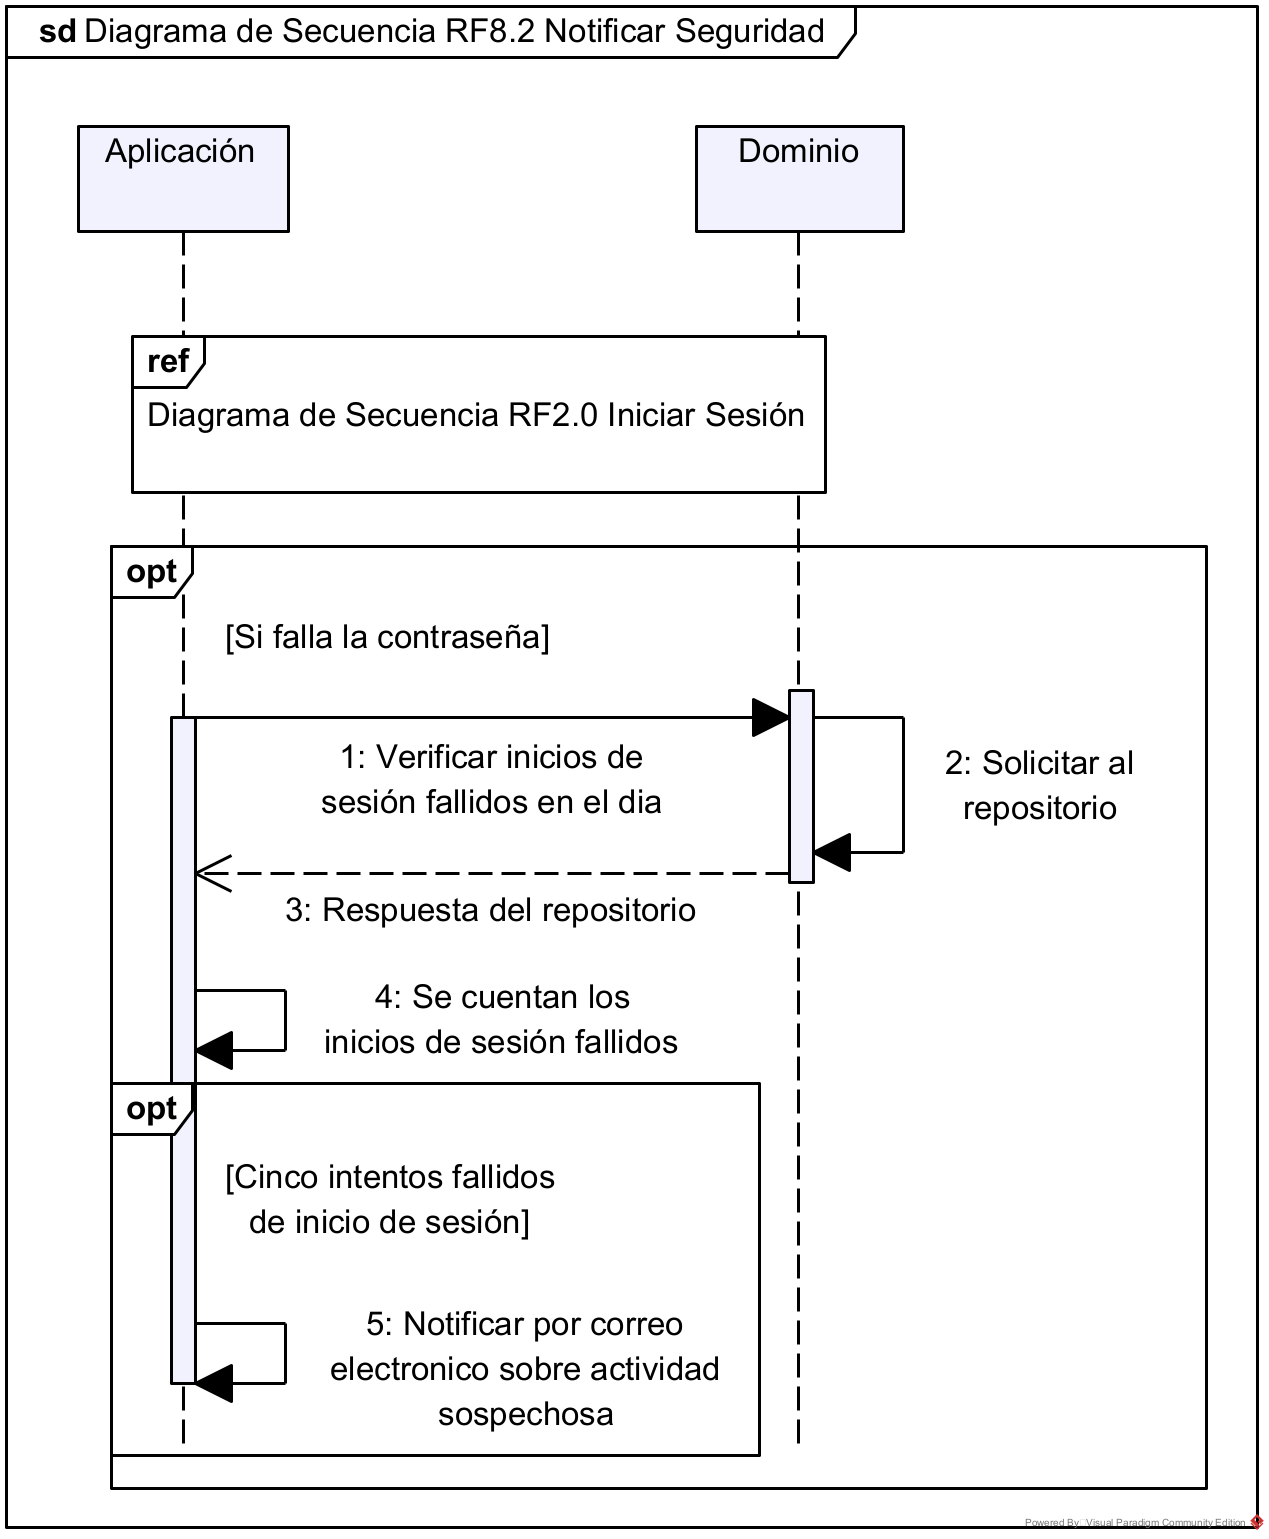
\includegraphics[width=0.8\textwidth]{UML/Secuencia/Diagrama de Secuencia RF8.2 Notificar Seguridad.png}
\end{figure}


\begin{figure}[H]
	\centering
	\caption{Diagrama de Secuencia para Crear Observación (RF9.1).}
 \includegraphics[width=0.8\textwidth]{UML/Secuencia/Diagrama de Secuencia RF9.1 Crear Observación.png}
\end{figure}


\begin{figure}[H]
	\centering
	\caption{Diagrama de Secuencia para Consultar Observación (RF9.1).}
 \includegraphics[width=0.8\textwidth]{UML/Secuencia/Diagrama de Secuencia RF9.2 Consultar Observación.png}
\end{figure}

% =================================================
% =================================================

\subsection{Diagramas de Actividades}

\begin{figure}[H]
    \centering
    \caption{Diagrama de Actividad para el Registro (RF1.0).}
    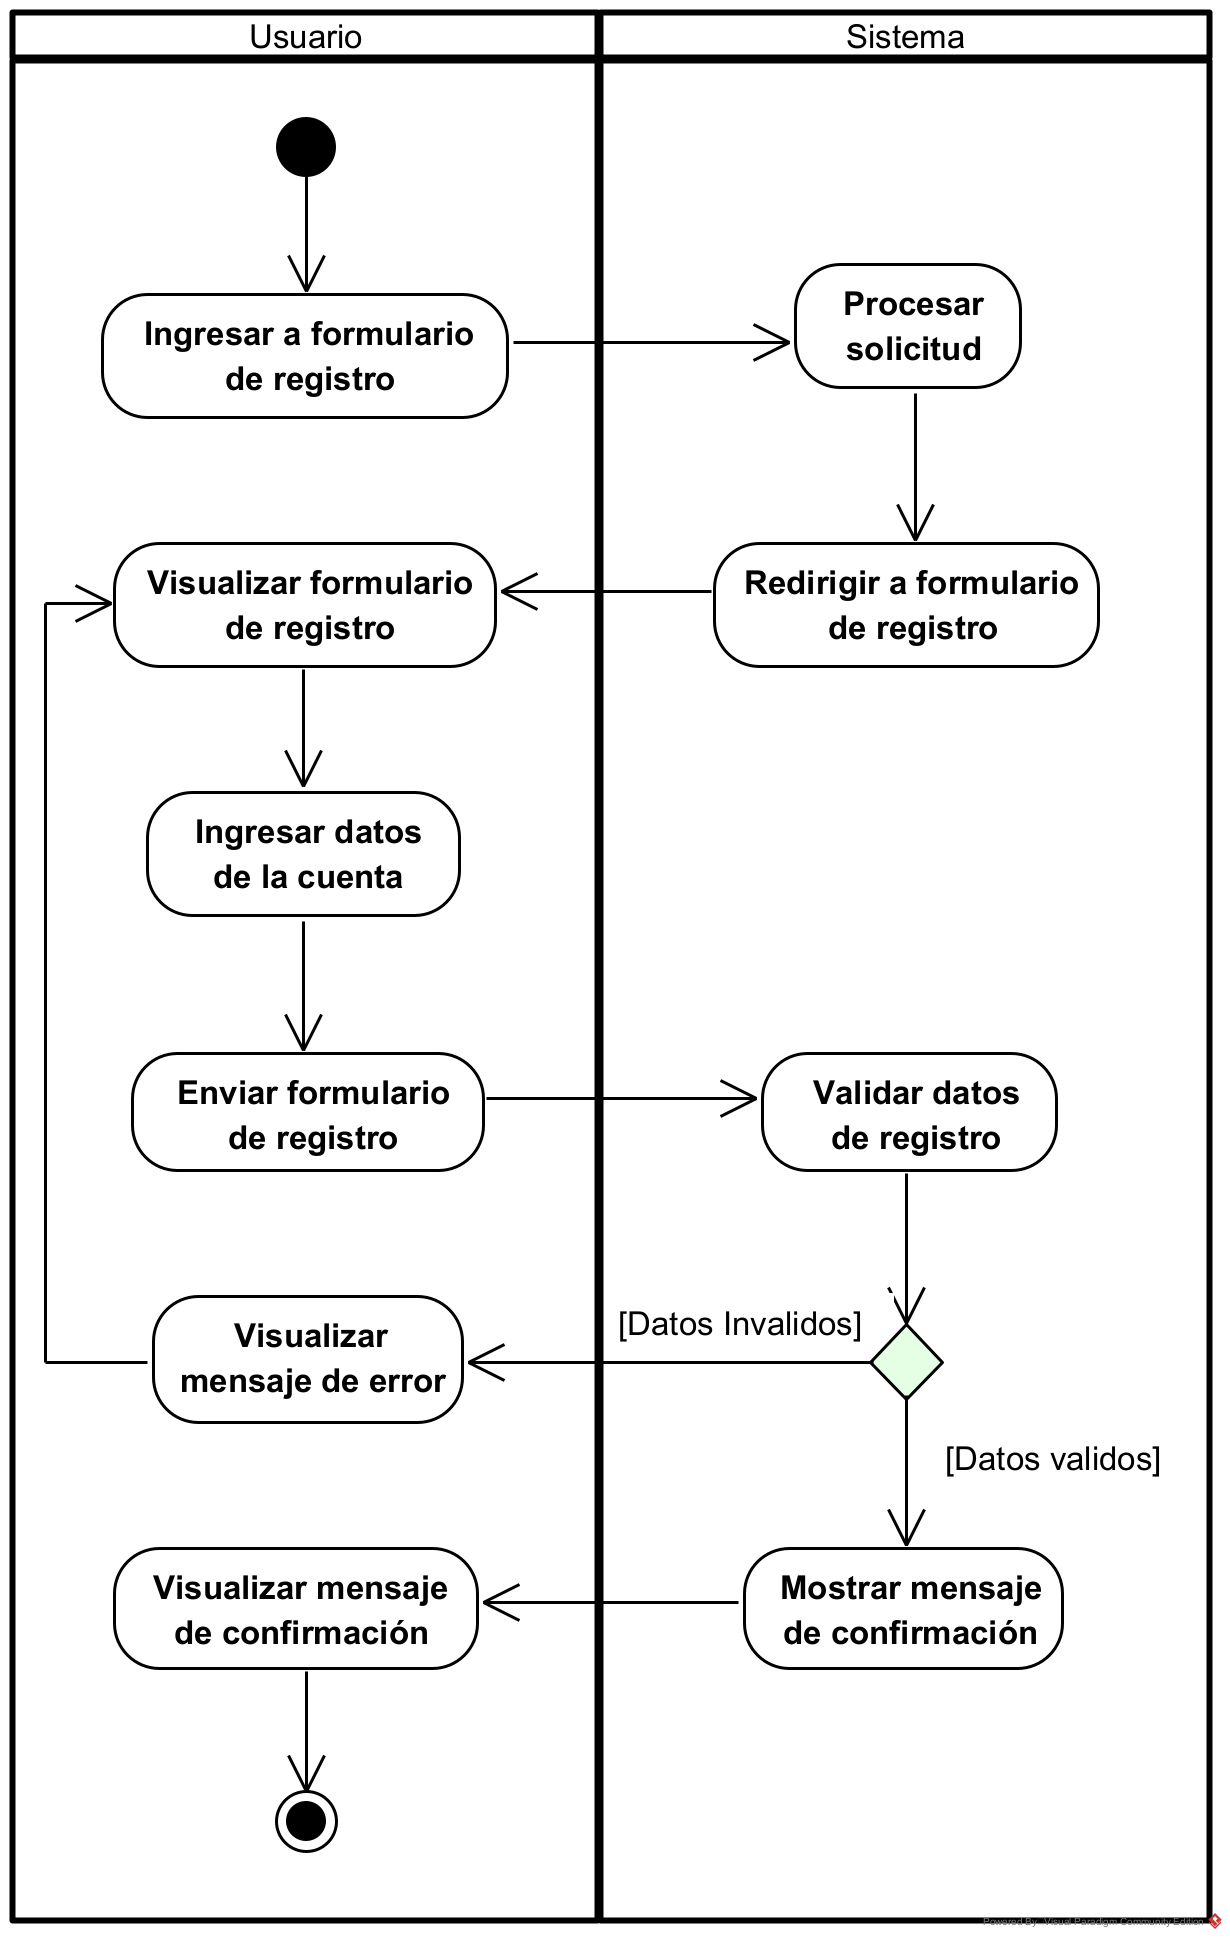
\includegraphics[width=0.7\textwidth]{UML/Actividad/Diagrama de Actividad RF1.0 Registro.png}
\end{figure}


\begin{figure}[H]
    \centering
    \caption{Diagrama de Actividad para Solicitar Código (RF1.1).}
 \includegraphics[width=0.6\textwidth]{UML/Actividad/Diagrama de Actividad RF1.1 Solicitar Código.png}
\end{figure}


\begin{figure}[H]
	\centering
	\caption{Diagrama de Actividad para Iniciar Sesión (RF2.0).}
 \includegraphics[width=0.7\textwidth]{UML/Actividad/Diagrama de Actividad RF2.0 Iniciar Sesión.png}
\end{figure}


\begin{figure}[H]
	\centering
		\caption{Diagrama de Actividad para Cerrar Sesión (RF2.1).}
	\includegraphics[width=0.65\textwidth]{UML/Actividad/Diagrama de Actividad RF2.1 Cerrar Sesión.png}
\end{figure}


\begin{figure}[H]
	\centering
	\caption{Diagrama de Actividad para Recuperar Contraseña (RF2.2).}
 \includegraphics[width=0.8\textwidth]{UML/Actividad/Diagrama de Actividad RF2.2 Recuperar Contraseña.png}
\end{figure}


\begin{figure}[H]
	\centering
	\caption{Diagrama de Actividad para Crear Cámara (RF3.1).}
 \includegraphics[width=0.8\textwidth]{UML/Actividad/Diagrama de Actividad RF3.1 Crear Cámara.png}
\end{figure}


\begin{figure}[H]
	\centering
		\caption{Diagrama de Actividad para Activar Cámara (RF3.1.1).}
	\includegraphics[width=0.8\textwidth]{UML/Actividad/Diagrama de Actividad RF3.1.1 Activar Cámara.png}
\end{figure}


\begin{figure}[H]
	\centering
		\caption{Diagrama de Actividad para Activar Hardware (RF3.1.1).}
	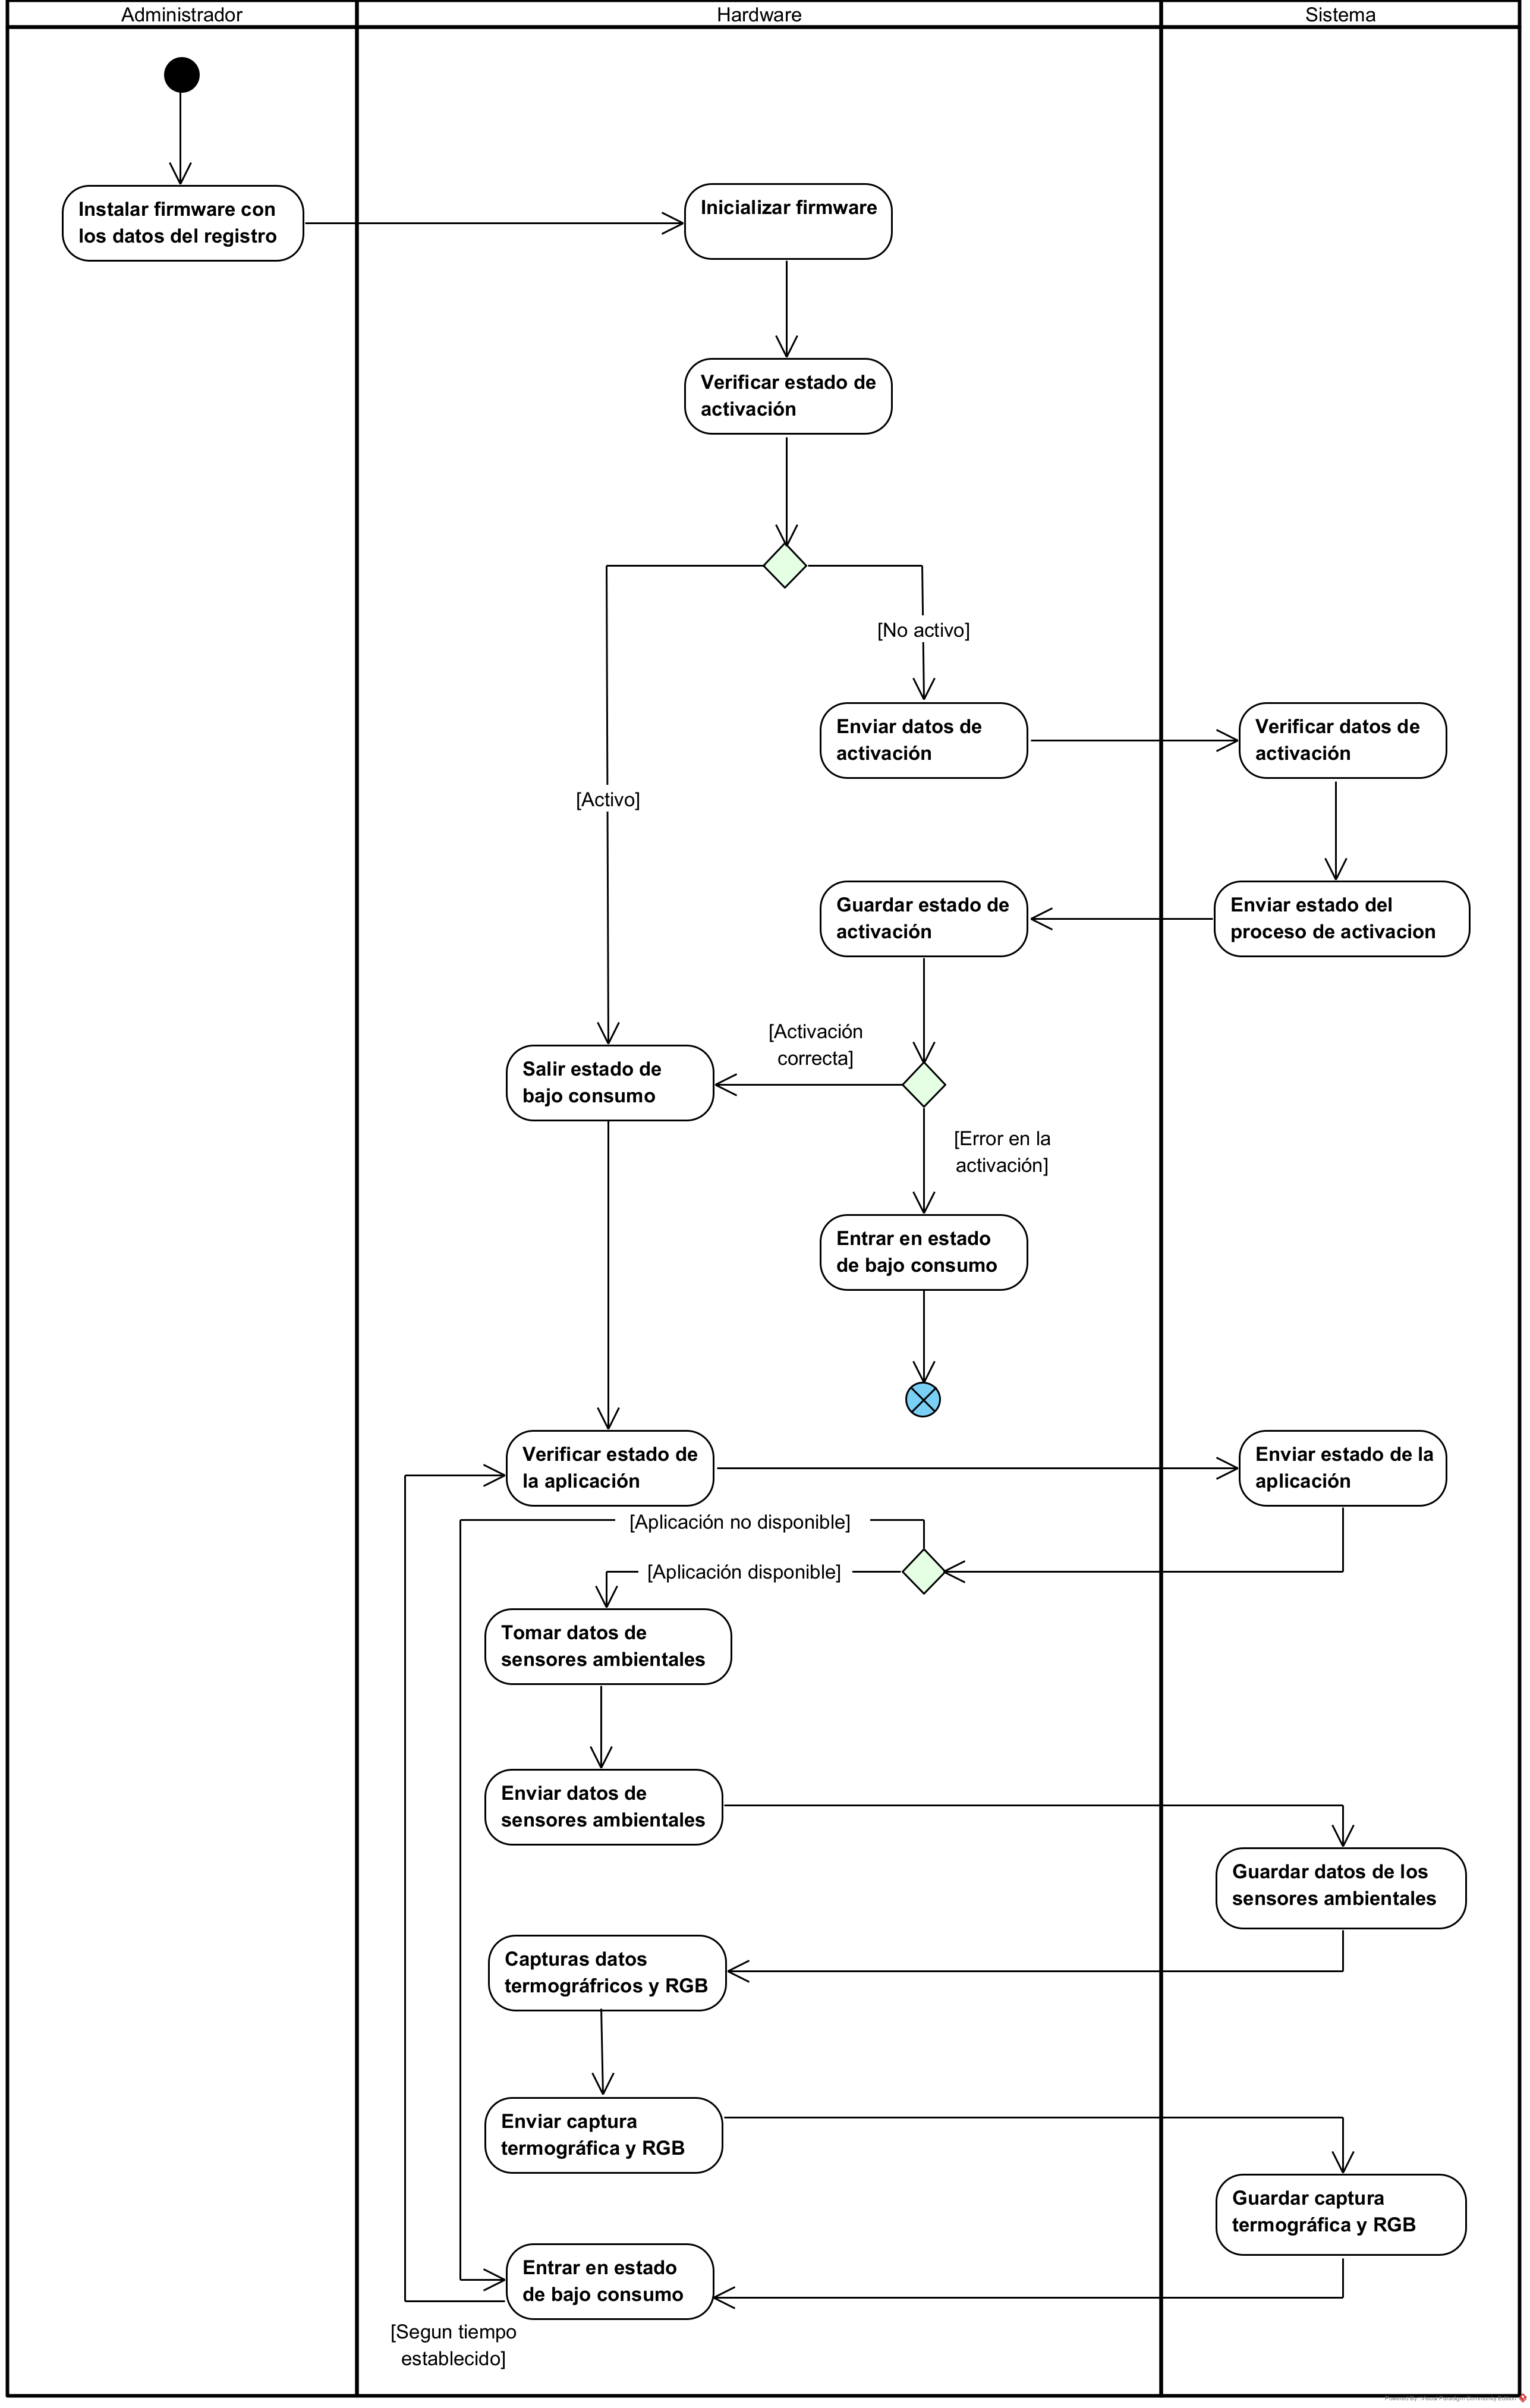
\includegraphics[width=0.8\textwidth]{UML/Actividad/Diagrama de Actividad RF3.1.1 Activar Hardware.png}
\end{figure}


\begin{figure}[H]
	\centering
	\caption{Diagrama de Actividad para Consultar Cámara (RF3.2).}
 \includegraphics[width=0.8\textwidth]{UML/Actividad/Diagrama de Actividad RF3.2 Consultar Cámara.png}
\end{figure}


\begin{figure}[H]
	\centering
	\caption{Diagrama de Actividad para Editar Cámara (RF3.3).}
 \includegraphics[width=0.8\textwidth]{UML/Actividad/Diagrama de Actividad RF3.3 Editar Cámara.png}
\end{figure}


\begin{figure}[H]
	\centering
		\caption{Diagrama de Actividad para Eliminar Cámara (RF3.4).}
\includegraphics[width=0.8\textwidth]{UML/Actividad/Diagrama de Actividad RF3.4 Eliminar Cámara.png}
\end{figure}


\begin{figure}[H]
	\centering
		\caption{Diagrama de Actividad para Consultar Perfil (RF4.1).}
	\includegraphics[width=0.8\textwidth]{UML/Actividad/Diagrama de Actividad RF4.1 Consultar Perfil.png}
\end{figure}


\begin{figure}[H]
	\centering
	\caption{Diagrama de Actividad para Editar Perfil (RF4.2).}
 \includegraphics[width=0.8\textwidth]{UML/Actividad/Diagrama de Actividad RF4.2 Editar Perfil.png}
\end{figure}


\begin{figure}[H]
	\centering
	\caption{Diagrama de Actividad para Eliminar Perfil (RF4.3).}
 \includegraphics[width=0.8\textwidth]{UML/Actividad/Diagrama de Actividad RF4.3 Eliminar Perfil.png}
\end{figure}


\begin{figure}[H]
	\centering
		\caption{Diagrama de Actividad para Cambiar Contraseña (RF4.4).}
	\includegraphics[width=0.8\textwidth]{UML/Actividad/Diagrama de Actividad RF4.4 Cambiar Contraseña.png}
\end{figure}


\begin{figure}[H]
	\centering
	\caption{Diagrama de Actividad para Agregar Integrante de Cultivo (RF4.5).}
 \includegraphics[width=0.8\textwidth]{UML/Actividad/Diagrama de Actividad RF4.5 Agregar Integrante Cultivo.png}
\end{figure}


\begin{figure}[H]
	\centering
	\caption{Diagrama de Actividad para Eliminar Integrante de Cultivo (RF4.6).}
 \includegraphics[width=0.8\textwidth]{UML/Actividad/Diagrama de Actividad RF4.6 Eliminar Integrante Cultivo.png}
\end{figure}

\begin{figure}[H]
	\centering
	\caption{Diagrama de Actividad para el Módulo de Mediciones (RF5.0).}
 \includegraphics[width=0.8\textwidth]{UML/Actividad/Diagrama de Actividad RF5.0 Módulo de mediciones.png}
\end{figure}


\begin{figure}[H]
	\centering
	\caption{Diagrama de Actividad para Crear Planta (RF6.1).}
 \includegraphics[width=0.8\textwidth]{UML/Actividad/Diagrama de Actividad RF6.1 Crear Planta.png}
\end{figure}


\begin{figure}[H]
	\centering
	\caption{Diagrama de Actividad para Consultar Planta (RF6.2).}
 \includegraphics[width=0.8\textwidth]{UML/Actividad/Diagrama de Actividad RF6.2 Consultar Planta.png}
\end{figure}


\begin{figure}[H]
	\centering
		\caption{Diagrama de Actividad para Editar Planta (RF6.3).}
	\includegraphics[width=0.8\textwidth]{UML/Actividad/Diagrama de Actividad RF6.3 Editar Planta.png}
\end{figure}


\begin{figure}[H]
	\centering
	\caption{Diagrama de Actividad para Eliminar Planta (RF6.4).}
 \includegraphics[width=0.8\textwidth]{UML/Actividad/Diagrama de Actividad RF6.4 Eliminar Planta.png}
\end{figure}


\begin{figure}[H]
	\centering
		\caption{Diagrama de Actividad para Generar Reporte (RF7.0).}
	\includegraphics[width=0.8\textwidth]{UML/Actividad/Diagrama de Actividad RF7.0 Generar Reporte.png}
\end{figure}


\begin{figure}[H]
	\centering
		\caption{Diagrama de Actividad para Descargar Reporte (RF7.1).}
\includegraphics[width=0.8\textwidth]{UML/Actividad/Diagrama de Actividad RF7.1 Descargar Reporte.png}
\end{figure}


\begin{figure}[H]
	\centering
		\caption{Diagrama de Actividad para Adjuntar Reporte (RF7.2).}
\includegraphics[width=0.8\textwidth]{UML/Actividad/Diagrama de Actividad RF7.2 Adjuntar Reporte.png}
\end{figure}


\begin{figure}[H]
	\centering
	\caption{Diagrama de Actividad para Notificar Planta (RF8.1).}
 \includegraphics[width=0.8\textwidth]{UML/Actividad/Diagrama de Actividad RF8.1 Notificar Planta.png}
\end{figure}


\begin{figure}[H]
	\centering
		\caption{Diagrama de Actividad para Notificar Seguridad (RF8.2).}
	\includegraphics[width=0.8\textwidth]{UML/Actividad/Diagrama de Actividad RF8.2 Notificar Seguridad.png}
\end{figure}


\begin{figure}[H]
	\centering
	\caption{Diagrama de Actividad para Crear Observación (RF9.1).}
 \includegraphics[width=0.8\textwidth]{UML/Actividad/Diagrama de Actividad RF9.1 Crear Observación.png}
\end{figure}


\begin{figure}[H]
	\centering
		\caption{Diagrama de Actividad para Consultar Observación (RF9.2).}
	\includegraphics[width=0.8\textwidth]{UML/Actividad/Diagrama de Actividad RF9.2 Consultar Observación.png}
\end{figure}

% =================================================
% =================================================

\subsection{Diagrama de Clases}
Incluir el diagrama con descripciones por cada clase.

% =================================================
% =================================================

\subsection{Diagrama de Despliegue}
\begin{figure}[H]
    \centering
    \caption{Diagrama de Despliegue del Sistema.}
    \label{fig:despliegue}
    \includegraphics[width=0.8\textwidth]{UML/Otros/Diagrama de Despliegue.png}
\end{figure}

% =================================================
% =================================================

\section{Diseño de los Casos de Prueba}
Texto sobre el diseño de casos de prueba utilizando SonarQube.

% =================================================
% =================================================

\section{Estimación de Recursos}
Texto sobre la estimación de recursos utilizando el método de puntos de función o puntos de casos de uso.

\section{Resultados de la Implementación del Software}
Texto sobre el resultado de implementar el software.

\section{Conclusiones y Recomendaciones del software}
Discusión, conclusiones y recomendaciones sobre el software y su integración.
         % Capítulo II: Documentación del Software
% Capítulo IV: Desarrollo y Caracterización del Hardware
\chapter{DOCUMENTACIÓN DEL HARDWARE}

\section{Introducción y Justificación del Hardware}
En este capítulo se presenta la importancia del hardware en el sistema de detección temprana de Botrytis cinerea, justificando la selección de cada componente y su contribución al funcionamiento global del sistema.

\section{Descripción de Componentes}
\subsection{Microcontrolador ESP32-S3-WROOM-1 N16R8}
Descripción del microcontrolador y sus características principales.

\subsection{Cámara termográfica MLX90640}
Descripción del sensor de termografía, sus especificaciones y función en la detección.

\subsection{Sensor de luz BH1750}
Detalle del sensor de luminosidad y su relevancia en el monitoreo ambiental.

\subsection{Sensor de humedad y temperatura DHT22}
Explicación del sensor de temperatura y humedad, resaltando su precisión y rango de medición.

\subsection{Cámara RGB OV2640}
Breve descripción de la cámara adicional y sus aplicaciones en el proyecto.

\subsection{Regulador de voltaje LM2596}
Descripción del regulador de voltaje y su importancia para garantizar la estabilidad del sistema.

\section{Metodología de Caracterización}
Esta sección describe el proceso sistemático para evaluar y validar el desempeño de cada componente y su integración en el sistema final.

\subsection{Evaluación y verificación de componentes}
\begin{itemize}
    \item \textbf{Definición de Parámetros de Evaluación:} Establecer los parámetros (por ejemplo, precisión, tiempo de respuesta y estabilidad) a medir para cada sensor y módulo.
    \item \textbf{Diseño de Protocolos de Prueba:} Elaborar procedimientos detallados para realizar pruebas de calibración y verificación en condiciones controladas.
    \item \textbf{Implementación de Ensayos Experimentales:} Ejecutar las pruebas en laboratorio, documentando condiciones ambientales, configuraciones y resultados obtenidos.
    \item \textbf{Análisis de Resultados:} Comparar los datos obtenidos con las especificaciones del fabricante y los requerimientos del proyecto.
\end{itemize}

\subsection{Configuración e Integración del Firmware}
\begin{itemize}
    \item \textbf{Diseño del Esquema de Integración:} Elaborar diagramas que muestren la conexión física entre el ESP32 y cada componente, indicando rutas de comunicación (I2C, SPI, etc.).
    \item \textbf{Configuración en Platform.io IDE:} Documentar el proceso de configuración, instalación de librerías, asignación de pines y gestión de interrupciones o tiempos de muestreo.
    \item \textbf{Pruebas de Integración:} Realizar pruebas para verificar la comunicación y correcta transmisión de datos entre el hardware y el firmware.
    \item \textbf{Documentación de la Integración:} Registrar todos los pasos y resultados obtenidos para facilitar futuras revisiones o ajustes.
\end{itemize}

\subsection{Validación y Análisis de Resultados}
En esta sección se evalúa el rendimiento global del sistema integrado mediante la comparación de datos experimentales controlados con los objetivos del proyecto. Se presentan datos, gráficos y análisis que demuestran el desempeño de cada componente y del sistema en conjunto, contrastándolos con los parámetros de referencia y registrando hallazgos para futuras revisiones.

\section{Implementación del Sistema Integrado}
Se describe la implementación práctica, incluyendo la integración final del hardware con el firmware, la calibración de sensores y la ejecución de pruebas en condiciones reales para ajustar y optimizar el sistema.

\section{Discusión}
Interpretación de los resultados finales obtenidos, identificando fortalezas y áreas de mejora, y estableciendo la relación entre el rendimiento del hardware y los objetivos del proyecto.
         % Capítulo IV: Desarrollo y Caracterización del Hardware
% Capítulo V: Estudio Experimental en Plantas de Arándano Biloxi
\chapter{ESTUDIO EXPERIMENTAL}

\section{Introducción y Objetivos del Estudio Experimental}
Se presenta el contexto del cultivo de arándano biloxi y la relevancia de detectar tempranamente Botrytis cinerea. Se definen los objetivos específicos del estudio experimental.

\section{Preparación del Hongo \textit{Botrytis cinerea}}
Descripción del protocolo para el manejo, cultivo y preparación del hongo, detallando medidas de seguridad y procedimientos para garantizar la viabilidad del patógeno.

\section{Diseño Experimental}
\begin{itemize}
    \item \textbf{Procedimiento de Infección:} Descripción de cómo se realizará la inoculación en las plantas.
    \item \textbf{Planificación de la Toma de Datos:} Definición del cronograma, frecuencia y condiciones bajo las cuales se efectuarán las mediciones.
    \item \textbf{Técnicas Utilizadas:} Detalle de las metodologías (incluyendo termografía) y herramientas empleadas para la captura de datos.
\end{itemize}

\section{Recolección y Análisis de Datos}
Metodología para la recopilación de datos experimentales, métodos estadísticos aplicados para el análisis comparativo entre plantas infectadas y de control, y presentación de resultados preliminares.

\section{Resultados y Discusión}
Presentación detallada de los hallazgos experimentales, análisis crítico de los resultados y comparación con los objetivos planteados en el estudio. Se discutirán las implicaciones de la detección temprana y su potencial para mejorar el manejo del cultivo.      % Capítulo V: Estudio Experimental en Plantas de Arándano Biloxi
% Capítulo VI: Resultados Integrados y Conclusiones Globales
\chapter{RESULTADOS Y CONCLUSIONES FINALES}

\section{Pregunta de investigación}
Integración de los resultados obtenidos en la caracterización del hardware, la documentación del software y el estudio experimental, resaltando los aspectos más relevantes y la coherencia entre las diferentes etapas del proyecto.

\section{Discusión General}
Análisis crítico de la consecución de los objetivos planteados, discusión de las fortalezas y limitaciones del sistema propuesto, y evaluación del impacto potencial de la implementación en un entorno real.

\section{Recomendaciones}
\begin{itemize}
    \item Sugerencias para la mejora del sistema basado en los resultados obtenidos.
    \item Propuestas para futuras investigaciones que puedan ampliar o profundizar el trabajo realizado.
    \item Consideraciones sobre la escalabilidad y adaptabilidad del sistema a otros contextos o cultivos.
\end{itemize}

\section{Conclusiones Finales}
\begin{itemize}
    \item Resumen de los logros y aportes del proyecto.
    \item Reflexión sobre los retos encontrados y las soluciones implementadas.
    \item Recomendaciones para futuras investigaciones y mejoras en el sistema.
\end{itemize}     % Capítulo VI: Resultados Integrados y Conclusiones Globales

% Bibliografía
\addcontentsline{toc}{chapter}{Bibliografía}
\bibliography{bibliografia}

% Anexos
\appendix  % Indica el inicio de los anexos

\chapter*{Anexos}
\addcontentsline{toc}{chapter}{Anexos}

% Configurar el contador de secciones para usar letras mayúsculas
\renewcommand{\thesection}{\Alph{section}}

% Personalizar el formato de los títulos de las secciones para que muestren 'Anexo A.'
\titleformat{\section}{\normalfont\Large\bfseries}{Anexo \thesection.}{1em}{}

% Anexos numerados que aparecerán en el índice general
\setcounter{section}{0}  % Reinicia el contador de secciones
\section{Código Fuente del Módulo Principal}
Incluir el manual de usuario...

\section{Manual de Usuario por Roles}
Incluir el manual de usuario...

\section{Manual de Instalación}
Incluir manual de instalación...

\section{Artículos de Resultados de Investigación}
Incluir artículos correspondientes...

\section{Certificaciones de Ponencias y Controles de Seguimiento}

\includepdfmerge[nup=1x2, pages={1}]{anexos/ponenciagab1.pdf,anexos/ponenciajuan1.pdf}

% Fin del Documento
\end{document}